\documentclass[12pt,bibliography=oldstyle,DIV=12,parskip=half-]{scrreprt}
% esto me setea la variable pdf dependiendo del valor de \pdfoutput, que es >0
% sólo cuando estoy usando pdflatex para compilar el documento
%% \newif\ifpdf
%% \ifnum\pdfoutput<0
%% \pdffalse\fi
%% \ifnum\pdfoutput=0
%% \pdffalse\fi
%% \ifnum\pdfoutput>0
%% \pdftrue\fi


%
% ===
% === Trick para detectar si el documento está siendo compilado con pdflatex
% ===
%
% Esto me setea la variable pdf dependiendo del valor de \pdfoutput, que es >0
% sólo cuando estoy usando pdflatex para compilar el documento. Con esto puedo
% hacer  \ifpdf {...} \fi, que se ejecuta colo cuando compilo con pdflatex.
%% \newif\ifpdf
%% \ifnum\pdfoutput<0
%% \pdffalse\fi
%% \ifnum\pdfoutput=0
%% \pdffalse\fi
%% \ifnum\pdfoutput>0
%% \pdftrue\fi
%
% ===
% === I18n / L10n
% ===
%
% babel me da separación de sílabas para palabras en el idioma que le paso como
%       argumento opcional.
\usepackage[spanish,es-tabla,english]{babel}
%
% inputenc define la codificación de caracteres del código fuente, acá utf8.
\usepackage[utf8]{inputenc}
%
% ===
% === Gráficos
% ===
% 
% pst-pdf me permite usar PSTricks con pdflatex. Necesito cargarlo sólo si está
%         definida la variable pdf, por eso está entre \ifpdf ... \fi
%\ifpdf\usepackage{pst-pdf}\fi
%
% color me permite usar colores en el documento.
\usepackage{color}
%
% graphicx me da el comando \includegraphics para insertar imágenes (?)
\usepackage{graphicx}
%
% pstricks es un conjunto de macros basadas en PostScript para TeX, en
%          castellano: me da un entorno pstricks y comandos que uso dentro de
%          éste, que me sirven para dibujar figuras/diagramas/etc de manera
%          relativamente simple.
%\usepackage{pstricks}
%
% pst-circ me da macros para pstricks que me dibujan elementos de circuitos
%\usepackage{pst-circ}
%
% pst-plot me provee de funciones de ploteo para pstricks
%\usepackage{pst-plot}
%
% pst-2dplot me sirve para plotear en pstricks, entorno pstaxes
%\usepackage{pst-2dplot}
%
% ===
% === Verbatims
% ===
%
% verbatim es una reimplementación de los entornos verbatim[*]
%          provee el comando \verbatiminput{archivo} y el entorno comment, que
%          hace que LaTeX ignore directamente todo lo que está adentro
%\usepackage{verbatim}
%
% moreverb implementa el entorno verbatimtab indentando los tabs que encuentre,
%          y también el entorno listing, que pone números de línea al verbatim.
%          Para cambiar el ancho de la tabulacion, uso
%          \renewcommand\verbatimtabsize{<ancho del tab>\relax}
%          También define el entorno boxedverbatim.
%\usepackage{moreverb}
%
% listings me da el entorno lstlisting con resaltado de sintaxis.
%          Para setear el lenguaje del código, hago \lstset{language=<lang>}
%\usepackage{listings}
%
% url es un verbatim para escribir URL's que permite linebreaks dentro de ésta.
%     para usarlo, \url{<URL>}
\usepackage{url}
%
% ===
% === Más packages
% ===
%
%% \usepackage{mdwlist}		%Para listas mas compactas
%% \usepackage{textcomp}		%Para algunos símbolos
%% \usepackage{colortbl}		%Para celdas de colores en tablas
%% \usepackage{fancyhdr}		%Para encabezados/pie
\usepackage{bbold}		%Fuente bb para modo math: \mathbb{R} = reales
\usepackage{dsfont}		%Fuente ds para modo math: \mathds{R} = reales
\usepackage{multirow}		%Para "combinar" celdas en tablas
\usepackage{float}		%Para mejorar cuadros, figuras, etc
%% \usepackage{fancybox}		%Para recuardos de texto con bordes "fancy"
%% \usepackage{dingbat}		%Para dingbats
%\usepackage{marginal}		%Para  notas al margen que no puedo hacer andar
\usepackage{amsmath}		%Para enornos matemáticos mas flexibles
%\usepackage{varwidth}		%varwidth es un minipage que se ajusta al ancho mínimo


\usepackage[backend=biber,sorting=none,style=ieee,eprint=false,url=false]{biblatex} %% style=ieee
%% requiere texlive-bibtex-extra en debian


\usepackage{enumitem}
\setlist{noitemsep}
%% \setlist[description]{noitemsep}
%% \setlist[enumerate]{noitemsep}
%% \setlist[itemize]{noitemsep}

\usepackage{tikz}
\usepackage{pgfkeys}
\usepackage{pgfgantt}

% typearea: uso con koma-script para ajustar márgenes de página.
% vars globales a setear en la clase koma-script: DIV=12, BCOR=margen de ``binding'' para double side
\usepackage{typearea}

% para poder usar footnotes p.ej, adentro de un tabular
\usepackage{footnote}
\makesavenoteenv{tabular}

% para tabulars mas lindos/legibles
\usepackage{booktabs}

%\usepackage{glossaries}

\usepackage[spanish]{algorithm2e}

% para highlight (comando \hl{})
\usepackage{soulutf8}

% para teoremans etc
\usepackage{amsthm}

% para tunear citations
%\usepackage[square,comma,numbers,sort&compress]{natbib}


% config.tex: configuraciones del documento
%\selectlanguage{spanish}		%Elijo idioma español

%Permitir que los entornos equation, align, etc permitan saltos de página
%\allowdisplaybreaks[1]

%Tweaks
%% \setlength{\parindent}{0mm}		%Sangría de 1a. línea
%% \setlength{\hoffset}{2.6mm}		%
%% \setlength{\voffset}{-5.4mm}		%
%% \setlength{\topmargin}{0mm}		%
%% \setlength{\oddsidemargin}{5mm}	%
%% \setlength{\evensidemargin}{5mm}	%
%% \setlength{\marginparsep}{5mm}	%
%% \setlength{\headheight}{12.5mm}	%
%% \setlength{\headsep}{2.5mm}		%
%% \setlength{\footskip}{10mm}		%
%% \setlength{\textwidth}{14.1cm}		%
%% \setlength{\textheight}{232mm}	%
%% \setlength{\fboxrule}{.1pt}
%% \setlength{\parskip}{.5\baselineskip}

%Colores
\definecolor{negro}	{cmyk}{0,0,0,1}
\definecolor{marron}	{cmyk}{0,.5,1,.41}
\definecolor{rojo}	{cmyk}{0,1,1,0}
\definecolor{naranja}	{cmyk}{0,.35,1,0}
\definecolor{amarillo}	{cmyk}{0,0,1,0}
\definecolor{verde}	{cmyk}{1,0,1,0}
\definecolor{azul}	{cmyk}{1,1,0,0}
\definecolor{violeta}	{cmyk}{.45,1,0,0}
\definecolor{gris}	{cmyk}{0,0,0,.5}
\definecolor{blanco}	{cmyk}{0,0,0,0}
\definecolor{dorado}	{cmyk}{0,.16,1,0}
\definecolor{plateado}	{cmyk}{0,0,0,.25}

%% \title{\titulo}
%% \author{\autor}
%% \date{\fecha}

% si uso pdflatex, me setea las propiedades del pdf de salida
%% \ifpdf\pdfinfo{/Title    (\tituloPDF)
%%                /Author   (\autorPDF)
%%                /Subject  (\asuntoPDF)
%%                /Keywords (\clavesPDF)}\fi

% comandos.tex
% en este archivo defino todos los comandos/environment que quiera usar en mi documento.
%
% ===
% === Comandos
% ===
% 
% T: para escribir texto común cuando en modo math
%    uso: \T{texto que aparecerá en letra normal}
\newcommand{\T}{\textrm}
%
% aclaracion: dibuja un recuadrito aclaratorio, como <quote> en HTML.
%             uso: \aclaracion{Texto...}
\newcommand{\aclaracion}[1]{%
\smallpencil\-\begin{minipage}{0.9\textwidth}
%\vspace*{6pt}
{#1}\smallskip\end{minipage}}
%
% consigna: parecido a aclaración, pero con texto _slanted_
%           uso: \consigna{Consigna...}
\newcommand{\consigna}[1]{%
\leftpointright\ \parbox[t]{0.9\textwidth}{\textsl{#1}\vspace{8pt}}}
%
% pinterno: para representar el producto interno entre los dos argumentos
%           uso: \pinterno{X}{Y}
\newcommand{\pinterno}[2]{%
\left\langle #1 , #2 \right\rangle}
%
% === Estilos de texto
%
% resalt: resaltado con fondo verde
%         uso: \resalt{texto resaltado}
\newcommand{\resalt}{\colorbox{yellow}}
%
% sfbf: texto en negrita + slanted
%       uso:
\newcommand{\sfbf}[1]{\textsf{\bfseries #1}}
%
% small bold sans-serif
\newcommand{\sbs}[1]{\textsf{\small\bfseries #1}}
%
% eng: itálica (para palabras en inglés)
%      uso: \eng{some English text}
\newcommand{\eng}{\textit}
%
% mean: significado de una sigla - slanted
%       uso: (...) SNCF: \mean{Société Nationale des Chemins de Fer Francais} ...
\newcommand{\mean}{\textsl}
\newcommand{\desc}{\textsl}
%
% defin: pone en negrita el texto, útil para definiciones
%        uso: \defin{asshole}: vulgar slang for anus
\newcommand{\defin}{\textbf}
%
% R, N: cambia la tipografía en modo math, probar para ver cómo quedan
%       uso: \R{R} , \N{N}
\newcommand{\R}{\mathds}
\newcommand{\N}{\mathbf}
\newcommand{\C}{\mathcal}
\newcommand{\B}{\boldsymbol}
%
% dx: para escribir d2y/dx2, etc
\newcommand{\dx}[2]{\frac{d^{#2}\!#1}{d\!x^{#2}}}
%
% dp: para escribir derivadas parciales d2y/dx2, etc
\newcommand{\dpar}[3]{\frac{\partial^{#3}#1}{\partial{#2}^{#3}}}
%
% dvar: para escribir derivadas totales d2y/d(VAR)2, etc
\newcommand{\dvar}[3]{\frac{d^{#3}#1}{d{#2}^{#3}}}
%
% evalen: para escribir (loquesea)|_{evaluado_en}
\newcommand{\evalen}[2]{\left.{#2}\right|_{#1}}
%
% lil: para escribir texto pequeño. más cómodo que { \footnotesize texto pequeño... }
%      uso: \lil{texto pequeño... }
\newcommand{\lil}[1]{\footnotesize #1}  %Para texto pequeñooo
%
% mono: escribe el texto que le paso como parámetro con letra de ancho fijo
%       uso: \mono{texto monoespaciado}
\newcommand{\mono}[1]{{\texttt{#1}}}
%
% === Símbolos
%
\newcommand{\y}{\wedge}			%Y (Lógica)
\newcommand{\ve}{\vee}			%O (Lógica)
\newcommand{\ent}{\supset}		%Entonces (Lógica)
\newcommand{\dimp}{\leftrightarrow}	%Doble implicativo, equivalencia (Lógica)
\newcommand{\sii}{\leftrightarrow}	%Si y sólo si (Lógica)
\newcommand{\equi}{\equiv}		%Equivalencia (Lógica)
\newcommand{\portanto}{\vdash}		%Por lo tanto (Lógica)
\newcommand{\por}{\cdot}		%Producto punto
\newcommand{\RR}[1][1]{\mathds{R}}	%R de reales
\newcommand{\hfi}{\hat{\phi}}           %fi con gorrito arriba
\newcommand{\bfi}{\bar{\phi}}           %fi con raya arriba
\newcommand{\hpsi}{\hat{\psi}}          %Letra griega psi con gorrito arriba
\newcommand{\II}{\B{I}}                 %w negrita
\newcommand{\KK}{\B{K}}                 %w negrita
\newcommand{\QQ}{\B{Q}}                 %w negrita
\newcommand{\YY}{\B{Y}}                 %w negrita
\newcommand{\Bg}{\B{g}}                 %w negrita
\newcommand{\nn}{\B{n}}                 %w negrita
\newcommand{\uu}{\B{u}}                 %w negrita
\newcommand{\vv}{\B{v}}                 %w negrita
\newcommand{\ww}{\B{w}}                 %w negrita
\newcommand{\xx}{\B{x}}                 %x negrita
\newcommand{\yy}{\B{y}}                 %y negrita
\newcommand{\zz}{\B{z}}                 %z negrita
\newcommand{\BPhi}{\B{\Phi}}            %\Phi negrita
\newcommand{\Balpha}{\B{\alpha}}        %\alpha negrita
\newcommand{\Bbeta}{\B{\beta}}          %\beta negrita
\newcommand{\Btheta}{\B{\theta}}        %\theta negrita
\newcommand{\Bxi}{\B{\xi}}              %\xi negrita
%
%
% ===
% === Environments
% ===
% 
% enunciado: un environment que básicamente tiene el mismo efecto que el
%            comando consigna.
%            uso: \begin{enunciado} ... contenido ... \end{enunciado}
\newenvironment{enunciado}
{\leftpointright\ \begin{varwidth}[t]{0.9\textwidth}\textsl}
{\end{varwidth}\vspace{8pt}}
%
% pvi: para tipear la definición de un problema de valor inicial/funciones
%      definidas de a trozos/etc directamente en el texto (sin necesidad de
%      cambiar a un modo matemático.
%      uso: \begin{pvi} linea1 \\ linea 2 \\ ... \end{pvi}
\newenvironment{pvi}{\begin{equation}\begin{cases}}
{\end{cases}\end{equation}}
%
% pvi*: comp pvi, pero sin número de ecuación
\newenvironment{pvi*}{\begin{equation*}\begin{cases}}
{\end{cases}\end{equation*}}
%
% verbatimsmall: un verbatim con letra más chica. usualmente queda bastante
%                mejor que el verbatim pelado.
%                uso: \begin{verbatimsmall} ........ \end{verbatimsmall}
\newenvironment{verbatimsmall}{\small\begin{verbatim*}}
{\end{verbatim*}}
%
% nota: escribe una aclaracion dentro del texto
\newenvironment{nota}{$$\left[\;\begin{minipage}{0.95\textwidth}\slshape}
{\end{minipage}\;\right]$$}
%
%
% ===
% === Comandos ``históricos''
% ===
%
%% %\begin{pspicture}
%% \def\tierra(#1){%Para dibujar el símbolo de tierra en el entorno PSTricks
%% 	\rput(#1){
%% 		\psdot(0,0)
%% 		\psline(0,0)(0,-0.45)
%% 		\psline(-0.5,-0.45)(0.5,-0.45)
%% 		\psline(-0.35,-0.6)(0.35,-0.6)
%% 		\psline(-0.2,-0.75)(0.2,-0.75)
%% 	}%
%% }
%% %\end{pspicture}

\newcommand{\codigo}[2]{%Para generar un recuadro con código
	%\setlength{\hrulewidth}{0.1pt}
	\begin{flushleft}
	\underline{#1}
	\begin{tabular}{@{\quad}|l}
		\begin{minipage}{.85\textwidth}\smallskip{#2}
	\end{minipage}\end{tabular}\end{flushleft}%
}

\newcommand{\filecodigo}[1]{%Insertar código verbatim desde un archivo
\codigo{#1}{\verbatiminput{#1}}}%Requiere el paquete verbatim
\newcommand{\filecodigobis}[1]{{\verbatiminput{#1}}}%Requiere el paquete verbatim

%% \newcommand{\grafico}[3][1]{%Para generar un plot de un archivo con coords.
%% %\def\deequis=#1
%% \begin{minipage}{0.5\textwidth}\begin{center}
%% \begin{pspicture}(6,5)
%% 	\psgrid[subgriddiv=1,gridlabels=0pt,gridwidth=.1pt](1,3)(1,1)(6,5)
%% 	\psset{xunit=5cm,yunit=2cm}
%% 	\fileplot[linewidth=1pt,linecolor=blue,origin={0.2,1.5}]{#2}
%% 	\psset{xunit=1cm,yunit=1cm}
%% 	\psaxes[Dx=#1,dx=5,Oy=-1,Dy=1,dy=2]{-}(0.9,1)(6,5)
%% 	\rput(4,0.4){\textsl{#3}}
%% \end{pspicture}\end{center}\end{minipage}}

%% \newcommand{\eqncode}[2]{%
%% \begin{center}
%% \begin{tabular}{l@{\hspace{0.5cm}}r}
%% \begin{minipage}{.4\textwidth}
%% \begin{equation*}
%% #1
%% \end{equation*}
%% \end{minipage}
%% &
%% \fbox{\begin{minipage}{.4\textwidth}
%% %\setlength{\parskip}{4mm}
%% \filecodigobis{#2}
%% \end{minipage}}
%% \end{tabular}
%% \end{center}
%% }

%% \newcommand{\eqncodeb}[2]{%
%% \begin{center}\begin{tabular}{l@{\hspace{0.5cm}}r}
%% \begin{minipage}{.4\textwidth}#1\end{minipage} &
%% \fbox{\begin{minipage}{.4\textwidth}\filecodigobis{#2}\end{minipage}}
%% \end{tabular}\end{center}}

%% \newenvironment{matemcode}[1]{\newline
%% \begin{tabular}{l@{\hspace{0.5cm}}r}
%% \begin{minipage}{.4\textwidth}
%% \parbox[t]{.4\textwidth}{\begin{equation*}#1\end{equation*}}\end{minipage}
%% &\begin{Sbox}\begin{minipage}{.4\textwidth}}
%% {\end{minipage}\end{Sbox}\fbox{\TheSbox}\end{tabular}\newline}

%% \newenvironment{encuadrar}[1]{\begin{Sbox}\begin{varwidth}{#1\textwidth}}
%% {\end{varwidth}\end{Sbox}\fbox{\TheSbox}}

%% \newenvironment{parboxenv}{\begin{Sbox}}
%% {\end{Sbox}\parbox[t]{.9\textwidth}{\TheSbox}}

% multicolumn y multirow
\newcommand{\mcol}[3]{\multicolumn{#1}{#2}{#3}}
\newcommand{\mrow}[3]{\multirow{#1}{#2}{#3}}

%% Serif .......................................................................
%%
%% New Century Schoolbook
%% \usepackage[T1]{fontenc}
%% \usepackage{fouriernc}
%%
%%
%% TeX Gyre Schola (New Century extendida)
%% \usepackage[T1]{fontenc}
%% \usepackage{tgschola}
%%
%%
%% Utopia
%% \usepackage[T1]{fontenc}
%% \usepackage{fourier}
%%
%%
%% Utopia (con MathDesign)
%% \usepackage[T1]{fontenc}
%% \usepackage[adobe-utopia]{mathdesign}
%%
%%
%% Computer Concrete
%% \usepackage[T1]{fontenc}
%% \usepackage{concmath}
%%
%%
%% Charter BT
 \usepackage[T1]{fontenc}
 \usepackage[bitstream-charter]{mathdesign}
%%
%%
%% Nimbus Roman (clon de Times)
%% \usepackage[T1]{fontenc}
%% \usepackage{nimbus}
%%
%%
%% TeX Gyre Termes (version mejorada de Nimbus Roman)
%% \usepackage[T1]{fontenc}
%% \usepackage{tgtermes}
%%
%%
%% GFS Bodoni
%% \usepackage[T1]{fontenc}
%% \usepackage[default]{gfsbodoni}
%%
%%
%% Baskervald ADF
%% \usepackage[T1]{fontenc}
%% \usepackage{baskervald}
%%
%%
%% Efont Serif -- descargar de http://openlab.jp/efont/serif/
%% \usepackage[T1]{fontenc}
%% \usepackage{efont,mathesf}
%% \renewcommand*\oldstylenums[1]{{\fontfamily{esfod}\selectfont#1}}
%%
%%
%%
%%
%%
%% Sans-Serif ..................................................................
%%
%%
%% Optima (clon de, URW Classico)
%% \usepackage[T1]{fontenc}
%% \renewcommand*\sfdefault{uop}
%%
%%
%% Avantgarde (clon de, URW Gothic)
%% \usepackage[T1]{fontenc}
%% \usepackage{avant}
%%
%%
%% TeX Gyre Adventor (version mejorada de Avantgarde)
%% \usepackage[T1]{fontenc}
%% \usepackage{tgadventor}
%%
%%
%% Nimbus Sans (clon de Helvetica)
%% \usepackage[T1]{fontenc}
%% \usepackage{nimbus}
%%
%%
%% Helvetica (clon de, Nimbus Sans)
%% \usepackage[T1]{fontenc}
%% \usepackage[scaled]{helvet}
%%
%%
%% TeX Gyre Heros (version mejorada de Nimbus Sans)
%% \usepackage[T1]{fontenc}
%% \usepackage{tgheros}
%%
%%
%% Boilinum
%% \usepackage[T1]{fontenc}
%% \usepackage{libertine}
%%
%%
%% Computer Modern Bright
%% \usepackage[T1]{fontenc}
%% \usepackage{cmbright}
%%
%%
%% Latin Modern Sans
%% \usepackage[T1]{fontenc}
%% \usepackage{lmodern}
%%
%%
%% Epigrafica
%% \usepackage[OT1]{fontenc}
%% \usepackage{epigrafica}
%%
%%
%%
%% Si quiero el documento en sans en vez de Roman:
%% \renewcommand*\familydefault{\sfdefault}
%% ...............................................
%% 
%%
%%
%% Monospaced ..................................................................
%%
%%
%% Pandora Typewriter
%% \usepackage[T1]{fontenc}
%% \usepackage{pandora}
%%
%%
%% Letter Gothic
%% \usepackage[T1]{fontenc}
%% \usepackage{ulgothic}
%%
%%
%% Inconsolata
%% \usepackage[T1]{fontenc}
%% \usepackage{inconsolata}
%%

%
\addbibresource{res/bibliografia.bib}
%
\hyphenation{micro-RNA}
\hyphenation{micro-RNAs}
\hyphenation{mi-RNA}
\hyphenation{mi-RNAs}
%
\addtokomafont{descriptionlabel}{\small}
\setkomafont{subject}{\LARGE\usekomafont{disposition}}
\setkomafont{title}{\normalfont\slshape}
\setkomafont{subtitle}{\LARGE\usekomafont{disposition}}
%
%\renewcommand{\arraystretch}{1.0}
%
\setlength{\abovecaptionskip}{-10pt plus 3pt minus 2pt}
\setlength{\belowcaptionskip}{10pt plus 3pt minus 2pt}
%
\hypersetup{
    colorlinks,
    citecolor=black,
    filecolor=black,
    linkcolor=black,
    urlcolor=black
}
%
\newcommand{\e}{\emph}
\newcommand{\fr}[1]{(\autoref{#1})}
\newcommand{\iid}{independiente e idénticamente distribuido}
\newtheorem{definicion}{Definición}[chapter]
\newtheorem{lema}[definicion]{Lema}
\newcommand{\ntA}{\textrm{\mono{A}}{ }}
\newcommand{\ntC}{\textrm{\mono{C}}{ }}
\newcommand{\ntG}{\textrm{\mono{G}}{ }}
\newcommand{\ntU}{\textrm{\mono{U}}{ }}
\newcommand{\pairL}{\textrm{\mono{(}}{ }}
\newcommand{\pairR}{\textrm{\mono{)}}{ }}
\newcommand{\noPair}{\textrm{\mono{.}}{ }}
\newcommand{\dn}[1]{\textrm{\mono{#1}}{ }}
\newcommand{\bp}[2]{\textrm{\mono{#1-#2}}{ }}
\newcommand{\grad}[1]{\nabla{#1}}
%
%
%
%
%
\begin{document}
\selectlanguage{spanish}
%
% %%%%%%%%%%%%%%%%%%%%%%%%%%%%%%%%%%%%%%%%%%%%%%%%%%%%%%%%%%%%%%%%%%%%%%%%%%%%%
%
\titlehead{\center\large
  Universidad Nacional del Litoral\\
  Facultad de Ingeniería y Ciencias Hídricas
}
\title{\LARGE
  ``Desarrollo de un clasificador de secuencias de pre-microRNA
  mediante técnicas de Inteligencia Computacional''
}
\subject{
  Proyecto Final de Carrera\\
  Ingeniería en Informática
}
\subtitle{
  ~\\[.2ex]
  Informe final
  \\[.2ex]~
}
\author{
  Alumno: Mauro J. Torrez
}
\publishers{
  Director: Dr. Diego H. Milone
}
\date{
  ~\\[2em]
  \today
}
\renewcommand*{\titlepagestyle}{empty}
\maketitle
%
% %%%%%%%%%%%%%%%%%%%%%%%%%%%%%%%%%%%%%%%%%%%%%%%%%%%%%%%%%%%%%%%%%%%%%%%%%%%%%
% 
\tableofcontents
%
% %%%%%%%%%%%%%%%%%%%%%%%%%%%%%%%%%%%%%%%%%%%%%%%%%%%%%%%%%%%%%%%%%%%%%%%%%%%%%
% 
%
%
%
\chapter{Introducción}
\setcounter{page}{1}
%
%
%
\section{Acerca de los miRNA}
%
Hace aproximadamente una década se propuso que un tipo de pequeñas
moléculas previamente ignoradas, aunque presentes en grandes
cantidades en la célula, jugarían un papel decisivo en la reproducción
celular, promoviendo su diferenciación en distintos tipos de tejidos
y/o su permanencia en un estado particular de diferenciación
\cite{lee-mammal}.  Estas pequeñas moléculas de ácido ribonucleico
(\eng{RNA}, del inglés \emph{ribonucleic acid}), de unos $22$
nucleótidos $[\T{nt}]$ de longitud, se denominaron
\eng{microRNA} o \eng{miRNA}. Estudios posteriores han
demostrado que los miRNA ejercen una función reguladora de la
expresión génica celular \cite{bartel116} y están involucrados en
varios procesos genéticos dentro de la célula, como la transcripción
de mRNA (\emph{RNA mensajeros}) y la síntesis de proteínas
\cite{lili}.  Este efecto regulador puede tener gran implicancia en el
desarrollo y evolución de la enfermedad celular. Se ha demostrado que
los miRNA juegan un rol importante en la carcinogénesis
\cite{aurora}\cite{lili}, regulando la proliferación y muerte celular,
entre otras funciones como el metabolismo de las grasas en moscas, los
procesos de infección viral, y el control del desarrollo de flores y
hojas en plantas \cite{bartel116}\cite{lecellier}.

El debate acerca del número e identidad de los miRNA presentes en
diferentes genomas es una cuestión abierta: a modo de ejemplo, para el
caso del genoma humano se había estimado inicialmente que se
encontrarían unos pocos cientos de genes miRNA; posteriormente este
número ha sido revisado a unos 1000 \cite{sewer}\cite{chang}.
Actualmente, se encuentra que el número de miRNA descubiertos en
humanos duplica esta cifra \cite{gomes}. Asimismo, este número podría
ser mucho mayor si se considera que existen miRNA de evolución más
reciente, específicos a la especie humana \cite{sewer}.

Los miRNA se presentan naturalmente dentro de una molécula denominada
pre-miRNA o \emph{miRNA precursor}, de unos $70\T{nt}$ de
longitud, la cual contiene uno o más miRNA \emph{maduros} en su
secuencia. En la \autoref{horquilla} se representa en forma
esquemática la secuencia de una cadena de pre-miRNA y su
correspondiente \emph{estructura secundaria}. Esta estructura
secundaria viene dada por la forma en que la cadena de pre-miRNA se
\emph{pliega} sobre sí misma logrando una mayor estabilidad
molecular. Tal como se aprecia en la figura, se encuentra que en el
reino animal la estructura secundaria de un pre-miRNA conforma una
especie de \emph{horquilla} \cite{bartel116}\cite{sewer}.
\begin{figure}[H]
\smallskip\small\slshape\center
  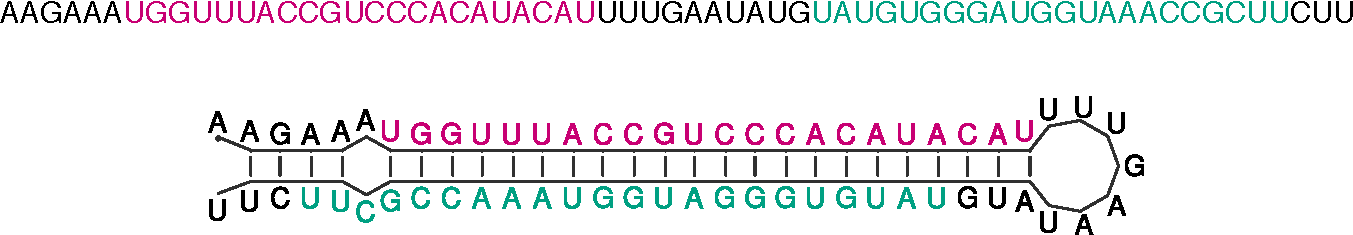
\includegraphics[width=.85\textwidth]{res/hsa-mir-299_ss.pdf}
  \caption{\small\slshape Secuencia
    (arriba) y estructura secundaria tipo horquilla (abajo) del
    pre-miRNA \textbf{hsa-mir-299}.  }
  \label{horquilla}
\end{figure}

%% Teniendo en cuenta que estas predicciones consideran sólo aquellos
%% miRNA que se encuentran conservados entre especies relativamente
%% distantes (como primates y roedores) y no aquellos de evolución más
%% reciente \cite{sewer}, el número de miRNA en humanos podría ser mucho
%% mayor que estas estimaciones.
%% La base de datos miRBase \cite{mirbase2}\cite{mirbase3}
%% recopila el conjunto de (pre-)miRNA conocidos hasta la
%% fecha. En la última versión disponible (r. 19, agosto de 2012) se listan
%% 21264 pre-miRNA experimentalmente validados, conteniendo un total de
%% 25141 miRNA maduros, para 193 especies diferentes.

La identificación de pre-miRNAs es el paso previo a la identificación
de miRNAs maduros. La primera opción para la identificación de nuevos
pre-miRNA son las pruebas experimentales de laboratorio. Sin embargo,
sólo aquellos pre-miRNA abundantes pueden ser detectados mediante esta
técnica de forma fiable. Esto implica que aquellos pre-miRNA con un
bajo nivel de expresión, que se expresan en tejidos específicos y/o
que se presentan sólo en determinados estadíos de desarrollo celular
pueden ser fácilmente ignorados mediante la técnica experimental
\cite{ding}\cite{xu}. En pos de superar estas dificultades propias del
método experimental es que surgen técnicas computacionales para
encontrar aquellos pre-miRNA que son específicos a determinados tipos
de tejidos o estadíos de desarrollo celular, y aquellos escasamente
expresados \cite{sheng}\cite{xu}.
%
%
%
\section{Clasificación de pre-miRNA}
%
Los métodos computacionales para clasificación de pre-miRNA se basan
en técnicas Aprendizaje Automático, una de las principales disciplinas
de la Inteligencia Computacional.  En general, estas técnicas de
\emph{aprendizaje supervisado} permiten generar un modelo o
representación interna que describe las características propias de los
pre-miRNA a partir de un conjunto de datos de ejemplo denominado
\emph{conjunto de entrenamiento}.  El modelo generado en la etapa de
entrenamiento puede ser aplicado a nuevos conjuntos de datos,
generando de esta manera un \emph{clasificador} capaz de discriminar
aquellos pre-miRNA reales de aquellos elementos que no se corresponden
con un pre-miRNA verdadero. En el presente trabajo se utilizan dos
técnicas diferentes para la generación de un clasificador de
pre-miRNA: el \emph{Perceptrón Multicapa} \cite{mlp1}\cite{mlp2} y la
\emph{Máquina de Vectores de Soporte} \cite{svm}.

El Preceptrón Multicapa (\emph{MLP}, del inglés \eng{Multilayer
  Perceptron}) es un tipo de red neuronal artificial con propagación
hacia adelante, donde las neuronas se disponen en capas. La salida de
cada neurona se determina al aplicar una \emph{función de activación},
de tipo sigmoidea, a la suma ponderada de las salidas en la capa
anterior. Durante el entrenamiento del MLP se ajustan los pesos de
cada neurona mediante un algoritmo de aprendizaje basado en la
\emph{retropropagación} del error de clasificación, hasta obtener una
tasa de clasificación satisfactoria \cite{jain}.

La Máquina de Vectores de Soporte (\emph{SVM}, de su nombre en inglés
\eng{Support Vector Machine}) es un algoritmo de clasificación que se
basa en transformar, mediante una función de transformación llamada
\emph{núcleo}, el espacio $N$-dimensional de los datos de entrada en
otro espacio de dimensión $M: M\gg N$, donde se espera que los datos
sean linealmente separables mediante un hiperplano. El entrenamiento
consiste en encontrar el hiperplano óptimo de separación para el
conjunto de datos presentado \cite{bottou}.

El objetivo del presente trabajo es desarrollar un método de
clasificación de pre-miRNA completo, incorporando clasificadores SVM y
MLP.
%
%
%
%
%
%
%
%
%
%
%
%
%
%
%
%
%
%
%
%
%
%
%
%
%
%
%
%
%
%
\chapter{Fundamentos teóricos}
%
%% \hl{En el presente capítulo se introducen las nociones teóricas necesarias
%% para la comprensión del problema a tratar. 
%% Familiarizarse con los conceptos y notación relevantes.}
%
%
%
\section{La clasificación como forma de aprendizaje supervisado}
%
%% La tarea de clasificación trata de identificar la categoría a la
%% que pertenece una nueva observación o \e{instancia}, a partir de un
%% conjunto de datos de entrenamiento en el cual la pertenencia de cada
%% instancia a una \e{clase} (categoría) es conocida.
%
En el contexto de la Inteligencia Computacional, la clasificación es
un tipo de \e{aprendizaje supervisado}, en el cual el objetivo es
\e{inferir} una función que relaciona \e{datos de entrada} con una
\e{salida} a partir de una serie de ejemplos que conforman el llamado
\e{conjunto de entrenamiento}.  Un algoritmo que implementa la
clasificación se conoce como un \e{clasificador}. La función
matemática que transforma datos de entrada a una categoría,
implementada por el algoritmo de clasificación, se llama \e{modelo} (o
\e{hipótesis}).

Un clasificador es un tipo de \e{máquina de aprendizaje}, definida
como un algoritmo que analiza los datos del conjunto de entrenamiento
y produce una función de correspondencia (el modelo) que puede ser
usada para relacionar nuevos datos de entrada a un valor de salida.
De este modo, el clasificador es capaz de replicar el comportamiento
del sistema o proceso que pretende modelar, y se dice que el modelo
obtenido es capaz de \e{generalizar} a partir de los datos de
entrenamiento.
%
\subsubsection{Aprendizaje supervisado}
%
Formalmente, el aprendizaje supervisado se define como sigue: sean $X$
e $Y$ espacios vectoriales, y sea $(\xx,\yy)\in{}X\times{}Y$ un
\e{ejemplo} (correspondiente a una observación) que relaciona una
entrada $\xx\in{}X$ con la salida correspondiente $\yy\in{}Y$.

Se asume que existe una distribución de probabilidades fija y
desconcida $\nu$ sobre el producto $X\times Y$, llamada
\emph{distribución generadora} de los datos.  El aprendizaje
supervisado trata la extracción de propiedades de esta distribución a
partir de un número finito de variables aleatorias, denominadas
\e{ejemplos}, que conforman el conjunto de datos de entrenamiento
%
\begin{align}
  D = \left((\B{x}_1,\yy_1),\ldots,(\B{x}_\ell,\yy_\ell)\right) \in
  \mathcal{D}=\bigcup_{\ell=1}^\infty (X\times Y)^\ell,
\end{align}
%
%% donde $\C{D}$ es el conjunto de todos los conjuntos de entrenamiento
%% posibles.
que se considera como una muestra independiente e idénticamente
distribuida de $\nu$, esto es, $D\sim\nu$.
%
\subsubsection{Modelo}
%
La extracción de propiedades de $\nu$ se efectúa mediante un modelo
$h:X\rightarrow{}Y$. En un problema de clasificación, $Y$ es un
conjunto discreto y finito, donde cada valor posible de $Y$ se
corresponde con una \emph{clase}. El caso más básico e importante es
la \e{clasificación binaria}, en la que se consideran sólo dos valores
en $Y$, comúnmente $+1$ y $-1$.
%
\subsubsection{Máquina de aprendizaje}
%
Sea $\C{H}=\{h:X\rightarrow Y\}$ el conjunto de todos los modelos
posibles. Una máquina de aprendizaje es una transformación
%
\begin{align}
  A:\mathcal{D}\rightarrow\C{H}
\end{align}
%
que relaciona un conjunto de datos a un modelo.
%% \footnote{En todos los
%% casos, se considera el tipo de aprendizaje denominado
%% \emph{batch}, en el que la máquina de aprendizaje tiene acceso al
%% conjunto de entrenamiento completo en todo momento.}
La máquina de aprendizaje $A$ no es necesariamente una transformación
en sentido matemático, sino que en general consiste en un algoritmo
que efectúa el proceso denominado \e{entrenamiento}.

Un clasificador es una máquina de aprendizaje para la cual las salidas
posibles del modelo es un conjunto de valores discreto y finito.
En adelante, siempre que se hable de máquinas de aprendizaje se incluyen
los clasificadores dentro de esta denominación.
%
\subsubsection{Función de pérdida}
%
%% El objetivo del aprendizaje es lograr un bajo error de generalización.
%% Para un ejemplo $(\xx,y)\in{}D$ y una predicción correspondiente
%% $\hat{y}$ efectuada por un modelo $h$, la función de costo es una
%% función
%% \begin{align}
%%   L:X\times Y\times Y\rightarrow \RR^{\geq 0},
%% \end{align}
%% con la propiedad de que $y=y'$ implica $L(x,y,y')=0$.
Para un ejemplo $(\xx,\yy)\in{}X\times{}Y$, la función de pérdida mide
la cantidad de error del modelo $\hat{\yy}=h(\xx)$ mediante la
transformación $L(\xx,\yy,\hat{\yy})$.  Si la predicción resultante
del modelo $\hat{\yy}$ es correcta, el error es nulo. En la práctica,
la mayoría de las funciones de pérdida no dependen de la entrada
$\xx$, sino sólo de la predicción $\hat{\yy}$ y la clase $\yy$.

Algunas de las funciones de pérdida más comunes son:
\begin{align}
  \T{\e{Pérdida 0-1}:} &\qquad
    L(\yy,\hat{\yy})=\begin{cases}0,\quad{}\yy=\hat{\yy}\\
      1,\quad\T{en otro caso}\end{cases} \\
  \T{\e{Pérdida ``bisagra''}:} &\qquad
    L(\yy,\hat{\yy})=\max\{0,\yy-\hat{\yy}\}\\
  \T{\e{Error absoluto}:} &\qquad
    L(\yy,\hat{\yy})=|\yy-\hat{\yy}|\\
  \T{\e{Error cuadrático}:} &\qquad
    L(\yy,\hat{\yy})=(\yy-\hat{\yy})^2.
\end{align}
%
%
\subsubsection{Error de generalización}
%
El error de generalización
$\mathcal{R}_\nu:\C{H}\rightarrow\RR^{\geq0}$ de un modelo $h$ se
define a partir de la función de pérdida $L$ según
%
\begin{align}
  \mathcal{R}_\nu=\mathds{E}_\nu\left[L(x,y,h(x))\right]
  =\int_{X\times Y} L(x,y,h(x))\, d\nu(x,y).
\end{align}
%
Como se puede ver, para el cálculo de este error se requiere conocer
la distribución generadora de datos $\nu$, justamente la incógnita que
se trata de aproximar mediante el aprendizaje supervisado.

Entonces, la aplicación del concepto de error de generalización es
teórica: cuando el problema está bien planteado y la máquina de
aprendizaje es \e{consistente}, una aproximación del error de
generalización convergerá a un valor estable $\C{R}^*$ para modelos
obtenidos sucesivamente con tamaños de conjuntos de datos mayores.
%
%
%% Sin embargo, es de esperar que un buen modelo $y=h(x)$ que aproxime la
%% distribución $\nu$ presente un error de generalización \e{similar} a
%% aquel de la distribución original $\nu$.
%
%% Dado que todo el conocimiento que se tiene del problema 
%% a resolver es un conjunto finito de datos de ejemplo, una muestra
%% cuya probabilidad también es desconocida, el principal inconveniente al
%% desarrollar/implementar una máquina de aprendizaje (clasificador)
%% resulta en ajustar correctamente el modelo dada esta incógnita.
%% \begin{enumerate}
%% \item Se deberá contar con una estimación lomás certera posible del
%%   error de generalización
%% \item Se deberá saber cuándo cortar el entrenamiento de modo de evitar
%%   el sobreajuste (ver abajo)
%% \item Se deberán elegir parámetros adecuados, si los hubiere, que
%%   generen un modelo factible (más adelante).
%% \end{enumerate}
%
%
\subsection{Entrenamiento}
%
Todo el conocimiento que se tiene sobre la distribución generadora de
datos $\nu$ proviene del conjunto de datos finito
$D=\left(x_1,y_1),\ldots,(x_\ell,y_\ell)\right)$.
Este conjunto de datos define una distribución empírica
%
\begin{align}
  \hat{\nu}=\frac{1}{\ell}\sum_{i=1}^{\ell}\delta_{(x_i,y_i)}(x,y)
\end{align}
%
donde $\delta_{(x,y)}$ denota el delta de Dirac en
$(x,y)\in{}X\times{}Y$.  Esta distribución conduce a la definición del
\e{error de entrenamiento} como el error de un modelo $h$ sobre los
datos de entrenamiento en $D$:
%
\begin{align}
  \hat{\C{R}}_D(h)=E_\T{entrenamiento}=\R{E}_{\hat{\nu}}[L(x,y,h(x))]
  =\frac{1}{\ell}\sum_{i=1}^\ell L(x_i, y_i, h(x_i)).
\end{align}
en donde $L$ es una \e{función de pérdida}.
%

El entrenamiento de una máquina de aprendizaje es consiste en
seleccionar el modelo con el mínimo error de entrenamiento
%
\begin{align}
  \hat{h}:=\arg \min \left\{ \hat{\C{R}}_D(h)\middle|h \in H\right\}.
\end{align}
%
Este procedimiento se conoce también como la minimización del riesgo
empírico, y define una máquina de aprendizaje
$A_H:\C{D}\rightarrow{}H$ para cada clase $H$ de modelo.
%
%
%
%\subsection{Error de entrenamiento vs error de generalización}
%
%
%
%% De manera intuitiva, se puede postular que el proceso de
%% \emph{entrenamiento} de una máquina de aprendizaje se trata de
%% minimizar el error de entrenamiento.  Sin embargo, no se debe perder
%% de vista que el conjunto de datos de entrenamiento $D$ es una variable
%% aleatoria y no se puede saber cuál es la probabilidad de la
%% observación. Además, se puede dar el caso que $D$ contenga
%% \emph{ruido} (datos erróneos).
%
%
\subsubsection{Sobreajuste}
%
%% Sin entrar en mayores detalles, la generación de un modelo por parte
%% de la máquina de aprendizaje es una secuencia de pasos que va
%% generando modelos intermedios a partir de la presentación de cada uno
%% de los ejemplos en $D$. En la secuencia de modelos ${h_1, h_2,
%%   \ldots}$ en general se tiene que los primeros modelos
%
Se dice que un modelo presenta \emph{sobreajuste} cuando éste describe
el conjunto de datos de entrenamiento en lugar de la relación
subyacente $\nu$ entre las variables de entrada y de salida.
Intuitivamente, se puede decir que existe sobreajuste cuando el modelo
``memoriza'' ejemplos del conjunto de aprendizaje en lugar de
``aprender'' la relación subyacente entre los datos.  El problema del
sobreajuste existe debido a que la máquina de aprendizaje no recibe
información acerca de la \e{probabilidad} de cada ejemplo observado,
ignorando el ruido y los efectos aleatorios en el conjunto de datos de
entrenamiento.
%
%% Un ejemplo dado por Liebniz \cite{liebniz} resulta esclarecedor en
%% este aspecto: dado un conjunto finito de puntos distribuidos al azar
%% sobre una hoja de papel, éste puede ser perfectamente explicado por
%% una curva polinómica que atraviesa todos estos puntos. Claramente,
%% dicha curva polinómica no resulta una explicación plausible, dado que
%% los puntos se han dispuesto sobre la hoja al azar.
%
%% Por todo esto, en general se tendrá que el error de entrenamiento es
%% una estimación fuertemente sesgada (``demasiado optimista'') del error
%% de generalización, y no se debe utlizar como una medida válida para
%% comparación de modelos.
%
%
\subsection{Estimación del error de generalización}
%
El error de generalización es la medida más acertada para comparar el
rendimiento de diferentes modelos sobre un conjunto de datos
determinado $D$ \hl{justificar}. Sin embargo, al ser un valor no
calculable se hace necesario estimarlo mediante medidas de error
alternativas.
%
\subsubsection{Error de prueba}
%
Una situación óptima se da cuando se dispone de una muestra
independiente e idénticamente distribuida a $\nu$ denominada
\e{conjunto de prueba}:
%
\begin{align}
  T=((\tilde{x}_1,\tilde{y}_1),\ldots,(\tilde{x}_N,\tilde{y}_N))\sim\nu^N,
\end{align}
%
para el cual se define el \e{error de prueba} (o \e{de test}) como la
pérdida media
%
\begin{align}
  E_{test}=\frac{1}{N}\sum_{n=1}^N
  L(\tilde{x}_N,\tilde{y}_N,h(\tilde{x}_N)).
\end{align}
%
Este error de prueba es una estimación no sesgada del error de
generalización verdadero $\C{R}_\nu(h)$, y puede ser utilzado para
comparar modelos.
%
%
\subsubsection{Método de retención}
%
En la práctica, la mayoría de las veces el conjunto de prueba $T$ no
viene dado como tal, y en cambio se genera un conjunto $T^*\subset{}D$
seleccionando ejemplos al azar del conjunto de entrenamiento $D$.  A
fin de que exista una cierta ``independencia''\footnote{Estrictamente,
  la independencia no existe en este caso, ya que la pertenencia de un
  ejemplo al conjunto de entrenamiento $D^*$ implica la no pertenecia
  al conjunto de prueba $T^*$.} de los datos en $T^*$ respecto del
conjunto de entrenamiento, se genera un nuevo conjunto de entrenamiento
$D^*\subset{}D:D^*\cap{}T^*=\emptyset$ que será usado para entrenar la
máquina de aprendizaje. El conjunto $D^*$ se denomina en ocasiones
\e{conjunto de estimación}.
Finalmente, el error de prueba puede ser estimado calculando el error
sobre el conjunto $T^*$. Este método es conocido como el \e{método de
  retención}.
%
%% Se particiona el conjunto de entrenamiento $T$ en dos subconjuntos
%% complementarios, considerados independientes e idénticamente
%% distribuidos $E$ (entrenamiento) y $V$ (conjunto retenido o de
%% validación), entrenando el clasificador con los elementos de $E$ y
%% estimando el error de generalización con la tasa de error al
%% clasificar los elementos de $V$.
%
%% Esta medida es un buen estimador del error de generalización real, y
%% usualmente los parámetros óptimos para la una máquina de aprendizaje
%% entrenada con $E$ son suficientemente buenos para una SVM entrenada
%% con el conjunto completo $T$.
%
%% Sin embargo, el método de retención presenta una alta varianza
%% respecto de la elección de $V$, en especial con conjuntos de datos
%% pequeños. Por otro lado, al aumentar el tamaño de $V$ se genera un
%% sesgo sobre la estimación al reducir los datos de entrenamiento en
%% $E$.
%
\subsubsection{Validación cruzada de $k$ iteraciones}
%
%% La validación cruzada permite mejorar los problemas del método de
%% retención, aunque la separación de los datos en
%% entrenamiento-validación sigue siendo arbitraria.
%
En un procedimiento de \emph{validación cruzada de $k$ iteraciones}
\cite{crossval}, el conjunto $D$ se subdivide en $k$ conjuntos
disjuntos $D_1,\ldots,D_k$ de tamaños similares.

%% La forma general de esta técnica se denomina validación cruzada de $k$
%% iteraciones (\e{k-fold cross validation}), y consiste en dividir el
%% conjunto de entrenamiento en $k$ particiones de tamaño similar, que
%% serán utilizadas de modo ``cruzado'' para entrenamiento y validación
%% en $k$ iteraciones.

%% Para cada $i=1,\ldots,k$ se entrena la SVM con $T\backslash T_i$ y se
%% computa la tasa de error $E_i$ sobre el conjunto correspondiente
%% $T_i$, obteniendo finalmente la tasa de error total $E=\sum_{i=1}^k
%% E_i$.  En la literatura de aprendizaje de máquina, el valor de $k$
%% varía normalmente entre 3 y 10, y un valor de $k=5$ puede considerarse
%% estándar \cite{hastie}.

En cada iteración, se entrena la máquina de aprendizaje con $k-1$
particiones, y se clasifican aquellos datos de la partición restante
(\e{de validación}) para obtener una medida de desempeño. Se repite el
procedimiento de modo que en cada iteración se utilice una partición
diferente para validación.

Una vez completado el proceso, se dispondrá de $k$ medidas de
desempeño de la máquina de aprendizaje. Estas medidas pueden ser
promediadas para obtener un estimador del desempeño de la máquina de
aprendizaje. Este estimador es una medida más acertada que el error de
entrenamiento para estimar el error de generalización del modelo.

El error de validación cruzada presenta una menor varianza que aquel
del método de retención, sin embargo, al no ser los subconjuntos $D_i$
independientes e idénticamente distribuidos entre sí, se introduce un
sesgo en la estimación del error de generalización.  Tal como en el
caso del método de retención, en conjuntos de datos pequeños el método
de validación cruzada presenta una alta varianza respecto de la
elección de diferentes $D_i$.

El costo computacional del método de validación cruzada es $k$ veces
aquel del método de retención.
%
\subsubsection{Validación cruzada dejando uno fuera}
%
En el método de validación cruzada ``clásico'' de $k$ iteraciones, se
tiene para valores pequeños de $k$ una reducción en la varianza y para
valores grandes una reducción del sesgo. En el extremo, cuando se
establece $k$ al número de elementos en $D$, se está ante un método de
\emph{validación cruzada dejando uno fuera}. La condición $k=l=|D|$
implica la reducción del sesgo a un valor mínimo, ya que se separa
sólo un elemento para validación.  Sin embargo la varianza obtenida
mediante este método es máxima.

Para obtener una estimación del error de generalización mediante este
método es necesario entrenar el clasificador $l$ veces, lo que deriva
en un costo computacional muy elevado. Sin embargo, para el caso de un
clasificador SVM existen técnicas para el cálculo eficiente del error
dejando uno fuera \cite{chapelle-vapnik, lee-keerthi}.
%% La importancia del método radica en
%% que para el caso SVM, es posible derivar en forma teórica un límite
%% superior al error calculado mediante este método \cite{CITAME}.
%
%
%
%
\subsection{Regularización}
%
Al minimizar el error de entrenamiento se produce una tendencia al
sobreajuste, lo que se traduce en un rendimiento de generalización
subóptimo. Este sobreajuste genera fronteras de decisión relativamente
complejas para problemas que en realidad tienden a ser más simples.
Esto se condice con un principio a menudo referido como la ``navaja de
Ockam'':
%% ``\emph{entia non sunt multiplicanda praeter necessitatem}''
``las entidades no deben multiplicarse más allá de lo necesario'',
afirmando que las explicaciones simples son más plausibles y los
modelos sencillos más explicativos y más confiables que los
complicados.

La regularización consiste en forzar la simplicidad del modelo, y es
una de las estrategias principales utilizadas para evitar el
sobreajuste del modelo generado por la máquina de aprendizaje. Existen
dos formas comunes para incorporar simplicidad en el modelo:
%
\begin{itemize}
\item Limitar el modelo a una subclase de funciones simples.
\item Añadir un término de penalización por complejidad al objetivo
  del error de entrenamiento.
\end{itemize}
%
El segundo enfoque requiere que podamos medir la ``complejidad'' del
modelo. Ambos procedimientos regularizan el proceso de aprendizaje, ya
que favorecen las hipótesis más simples.

Cuando el entrenamiento de la máquina de aprendizaje es un proceso
gradual, una técnica alternativa de regularización consiste en
abortar el proceso de entrenamiento al momento que se detecta
que el error de generalización empieza a incrementarse.

Se debe notar que la regularización en general entra en conflicto con
la minimización del error de entrenamiento, y un modelo regularizado
cometerá más errores sobre el conjunto de entrenamiento que un modelo
no regularizado.  Sin embargo, se ha de esperar que el modelo
regularizado tenga mayor capacidad de generalización.
%
%
%
\subsection{Medidas de evaluación de un clasificador binario}
%
La evaluación de un clasificador binario se efectúa mediante una serie
de medidas que se calculan a partir del resultado de clasificar un
conjunto de prueba con elementos cuya clase es conocida.  El resultado
de aplicar el clasificador al conjunto de prueba con $N$ elementos se
caracteriza según las siguientes medidas:
%
\begin{itemize}[style=nextline]
  \item\emph{Verdaderos positivos (VP)}: número de elementos de clase
    positiva correctamente clasificados como positivos.
  \item\emph{Verdaderos negativos (VN)}: número de elementos de clase
    negativa correctamente clasificados como negativos.
  \item\emph{Falsos positivos (FP)}: número de elementos de clase
    negativa erróneamente clasificados como positivos.
  \item\emph{Falsos negativos (FN)}: número de elementos de clase
    positiva erróneamente clasificados como negativos.
\end{itemize}
%
Estas cuatro medidas conforman la llamada \emph{matriz de confusión}
característica del clasificador, y dependen en todos los casos del
número de elementos positivos y negativos presentes en el conjunto de
prueba.
%
\subsubsection{Sensibilidad y especificidad}
%
A partir de los valores de la matriz de confusión se definen las
medidas de \emph{sensibilidad ($SE$)} y \emph{especificidad ($SP$)}:
%
\begin{align*}
SE & = \frac{VP}{VP+FN}, & SP & = \frac{VN}{VN+FP}.
\end{align*}
%
En forma intuitiva, la sensibilidad \hl{tambien tpr, recuento}
indica la \emph{tasa de acierto}
al clasificar elementos de clase positiva, y la especificidad
representa la tasa de acierto al clasificar patrones de clase
negativa.  Ambas medidas son independientes del número de elementos
presentes en el conjunto de prueba, aunque no de la proporción entre
elementos positivos y negativos.

En la mayoría de problemas de clasificación ``en la vida real'',
se encuentra que las clases positiva y negativa \e{no son separables}
debido a razones diversas. Esta no separabilidad implica que siempre
habrá una proporción de falsos positivos y falsos negativos al
utilizar el clasificador.
La importancia de las medidas de sensibilidad y especificidad es que
permiten elegir, por ejemplo, el clasificador con menor cantidad de
falsos negativos, una característica deseable en detectores de
patógenos en bancos de sangre y detectores de explosivos en
aeropuertos.
%
\subsubsection{Otras medidas de desempeño}
%
En muchos problemas donde no se especifican requerimientos de
sensibilidad o especificidad del clasificador, se aconseja la
utilización de una medida única que maximice el rendimiento de
clasificación en general. La medida más simple puede ser un simple
promedio de la sensibilidad y la especificidad, sin embargo,
comúnmente se utiliza la media geométrica $G_m$, definida por
%
\begin{align*}
G_m & = \sqrt{SE\cdot SP}.
\end{align*}
%
Otras medidas comúnmente utilizadas para evaluación de un clasificador
binario son
%
  \begin{align*}
    \T{Precisión} && Pr &=\frac{VP}{VP+FP},\\
    \T{Exactitud} && Ac &=\frac{VP+VN}{VP+FP+VN+FN},\\
    \T{Valor-F}   && F  &=\frac{Pr\cdot{}SE}{Pr+SE}, \\
    \parbox{4cm}{Coeficiente de correlación de Matthews} &&
    MCC &= \frac{VP\cdot{}VN-FP\cdot{}FN}{\sqrt{(VP+FP)(VP+FN)(VN+FP)(VN+FN)}}.
  \end{align*}
%
%
%
\section{Hiperparámetros}
%
El entrenamiento de la máquina de aprendizaje puede explicarse como un
algoritmo de optimización que selecciona un modelo óptimo $h^*$ que
ajuste al conjunto de datos $D$ a partir de una familia de funciones
candidatas $H\subset\C{H}$.

\st{En la práctica, se encuentra que las técnicas utilizadas de
aprendizaje de máquina son demasiado generales como para ajustar
automáticamente todas las variables que intervienen en el proceso de
la obtención del modelo óptimo.  En particular,} muchas técnicas de
aprendizaje de máquina dejan a criterio del usuario la selección de
parámetros tales como
%
\begin{itemize}
\item el subtipo de familias $H^*\subset{}H$ a utilizar como modelo,
\item parámetros que regular el método de entrenamiento,
\item la selección del algoritmo de optimización,
\item la velocidad de convergencia y precisión requerida del
  algoritmo,
\item la cantidad de regularización a aplicar al modelo.
\end{itemize}
%
De este modo, el proceso de entrenamiento requiere la especificación
de parámetros adicionales que regulan el algoritmo de optimización así
como determinadas propiedades requeridas del modelo a utilizar.
Este conjunto de parámetros adicionales se denomina
comúnmente como \e{hiperparámetros}, y de este modo, la máquina de
aprendizaje puede escribirse como una transformación
%
\begin{align}
  A:\C{D}\times\C{P}\rightarrow\C{H}
\end{align}
%
que recibe los datos en $D\in\C{D}$ y los hiperparámetros en un vector
$\Btheta=(\theta_1,\theta_2,\ldots)\in\C{P}$.

%% que regulan el
%% comportamiento del proceso de entrenamiento, tales como la tolerancia
%% a errores, el tiempo máximo de entrenamiento o la exactitud de la
%% solución requerida.

%% En la práctica, se encuentra que estos parámetros son determinantes a la
%% hora de conseguir un modelo que ajuste correctamente a los datos
%% disponibles.

%
\subsubsection{Optimización de hiperparámetros}
%
La optimización de hiperparámetros hace referencia a la selección de
un vector de hiperparámetros $\Btheta^*$ óptimo tal que se obtenga el
mejor modelo posible que ajuste a los datos en $D$ con bajo error de
generalización.

Este problema es similar al proceso de entrenamiento, pero el objetivo
es determinar hiperparámetros óptimos, y en general, es un algoritmo
que tiene la forma
%
\begin{enumerate}
\item Elegir parámetros $\Btheta$
\item Entrenar la máquina de aprendizaje
\item Medir el error del modelo obtenido
\item Repetir el proceso 1--3 hasta satisfacer un criterio de corte
\item Seleccionar el $\Btheta$ resultante a partir de los resultados
  obtenidos
\end{enumerate}
%
En muchos casos, este procedimiento se reduce simplemente a utilizar
el conocimiento experto sobre el problema a resolver y elegir valores
adecuados. Sin embargo, en problemas generales resulta común aplicar
alguna heurística més o menos automática para la elección de valore
óptimos de hiperparámetros.

%% In the context of machine learning, hyperparameter optimization or
%% model selection is the problem of choosing a set of hyperparameters
%% for a learning algorithm, usually with the goal of optimizing a
%% measure of the algorithm's performance on an independent data
%% set. Often cross-validation is used to estimate this generalization
%% performance.[1] Hyperparameter optimization contrasts with actual
%% learning problems, which are also often cast as optimization problems,
%% but optimize a loss function on the training set alone. In effect,
%% learning algorithms learn parameters that model/reconstruct their
%% inputs well, while hyperparameter optimization is to ensure the model
%% does not overfit its data by tuning, e.g., regularization.
%
%% Algorithms for hyperparameter optimization
%
%% Grid search
%
%% The traditional way of performing hyperparameter optimization has been
%% grid search, or a parameter sweep, which is simply an exhaustive
%% searching through a manually specified subset of the hyperparameter
%% space of a learning algorithm. A grid search algorithm must be guided
%% by some performance metric, typically measured by cross-validation on
%% the training set[2] or evaluation on a held-out validation set.
%
%% Since the parameter space of a machine learner may include real-valued
%% or unbounded value spaces for certain parameters, manually set bounds
%% and discretization may be necessary before applying grid search.
%
%% For example, a typical soft-margin SVM classifier equipped with an RBF
%% kernel has at least two hyperparameters that need to be tuned for good
%% performance on unseen data: a regularization constant C and a kernel
%% hyperparameter γ. Both parameters are continuous, so to perform grid
%% search, one selects a finite set of "reasonable" values for each, say
%
%%     C \in \{10, 100, 1000\}
%%     \gamma \in \{0.1, 0.2, 0.5, 1.0\}
%
%% Grid search then trains an SVM with each pair (C, γ) in the Cartesian
%% product of these two sets and evaluates their performance on a
%% held-out validation set (or by internal cross-validation on the
%% training set, in which case multiple SVMs are trained per
%% pair). Finally, the grid search algorithm outputs the settings that
%% achieved the highest score in the validation procedure.
%
%% Grid search suffers from the curse of dimensionality, but is often
%% embarrassingly parallel because typically the hyperparameter settings
%% it evaluates are independent of each other.[1] Bayesian Optimization
%
%% Bayesian Optimization is a methodology for the global optimization of
%% noisy black-box functions. Applied to hyperparameter optimization,
%% Bayesian optimization consists of developing a statistical model of
%% the function from hyperparameter values to the objective evaluated on
%% a validation set. Intuitively, the methodology assumes that there is
%% some smooth but noisy function that acts as a mapping from
%% hyperparameters to the objective. In Bayesian optimization, one aims
%% to gather observations in such a manner as to evaluate the machine
%% learning model the least number of times while revealing as much
%% information as possible about this function and, in particular, the
%% location of the optimum. Bayesian optimization relies on assuming a
%% very general prior over functions which when combined with observed
%% hyperparameter values and corresponding outputs yields a distribution
%% over functions. The methodology proceeds by iteratively picking
%% hyperparameters to observe (experiments to run) in a manner that
%% trades off exploration (hyperparameters for which the outcome is most
%% uncertain) and exploitation (hyperparameters which are expected to
%% have a good outcome). In practice, Bayesian optimization has been
%% shown[3][4][5][6] to obtain better results in fewer experiments than
%% grid search and random search, due to the ability to reason about the
%% quality of experiments before they are run.  Random Search
%
%% Since grid searching is an exhaustive and therefore potentially
%% expensive method, several alternatives have been proposed. In
%% particular, a randomized search that simply samples parameter settings
%% a fixed number of times has been found to be more effective in
%% high-dimensional spaces than exhaustive search.[1] Gradient Based
%% Optimization
%
%% For specific learning algorithms, specialized model selection
%% algorithms can be used. E.g., Chapelle et al. present a gradient
%% descent algorithm for minimizing the estimated generalization error of
%% a support vector machine.[7]
%% La forma más común de una máquina de aprendizaje estadístico es una
%% transformación

Un algoritmo de selección de hiperparámetros puede definirse entonces
como una transformación
%
\begin{align}
  S:\C{D}\times\C{P} %\times\T{\hl{Fobjetivo}}
  \rightarrow\C{P}
\end{align}
%
que, dado un conjunto de hiperparámetros iniciales $\Btheta_0$ y el
conjunto de entrenamiento $\C{D}$, invoca la máquina de aprendizaje en
sucesivas iteraciones hasta encontrar un vector de parámetros óptimos
$\Btheta^*$ que minimizan alguna medida de error de clasificación.

%% The general supervised learning problem can be stated as follows.
%% Given sample data $S=\{(x_i,y_i)\,|\,1 \leq i \leq \ell\}$ drawn from an
%% unknown distribution $p$ over $X \times Y$, the goal of binary
%% classification is to infer a hypothesis $h:X \to Y$ that minimizes the
%% expected risk
%%
%% \begin{align}
%%   R_p(h)= \int\limits_{X \times Y} L_{0-1}(y,h(x)) \, \text{d}
%%   p(x,y) ,
%% \end{align}
%%
%% where $L_{0-1}(y,z)$ is 0
%% if $y=z$ and 1 otherwise.

%% Cuando se tiene un algoritmo que genera un modelo $h$ dado un conjunto
%% de datos $D$, dicho algoritmo es una instancia de una máquina de
%% aprendizaje estadístico $A$. El proceso de determinar $A$ a partir de
%% $D$ se llama el \emph{entrenamiento} de la máquina de aprendizaje, de
%% ahí que $D$ se denomina \emph{conjunto de entrenamiento}.
%
%
%
%

%
\subsubsection{Función objetivo}
%

%% \subsection{Selección del modelo SVM}
%
%% Dado un conjunto de datos conocidos $T=\{(x_i,y_i)\}, i=1,\ldots,l$ a
%% utilizar como entrenamiento de una SVM, la \emph{selección del modelo}
%% de la SVM trata de encontrar respuesta a las preguntas:
%% \begin{itemize}
%% \item ¿Cuál kernel (y con qué parámetros) obtiene los mejores
%%   resultados de clasificación?
%% \item ¿Cuál es el valor óptimo del parámetro de regularización $C$?
%% \end{itemize}
%% Estas preguntas no son independientes entre sí, y no es posible dar
%% una respuesta universalmente válida para cualquier problema de
%% clasificación.

%% La elección de la función de kernel dependerá del conocimiento previo
%% que se tenga sobre los datos a clasificar: cuando se dispone este
%% conocimiento, se utiliza normalmente una familia de funciones de
%% kernel que logre una máxima separación entre clases para el problema
%% a tratar.  Cuando no se cuenta con información particular del
%% problema, resulta común la utilización de un kernel lineal o
%% gaussiano. De este modo, se acota la búsqueda de una función de kernel
%% óptima a un conjunto finito de funciones con sus respectivos
%% hiperparámetros. En adelante, se denominan \emph{hiperparámetros} al
%% conjunto de los parámetros propios de la función de kernel y el
%% parámetro de regularización $C$ y se denotan con el símbolo $\theta$:
%% $\theta = \{\theta^{\T{kernel}}, C\}$. Esta distinción se hace en pos de evitar
%% confusión con los parámetros $(\alpha, b)$ de la SVM obtenidos durante el
%% proceso de entrenamiento.

Para seleccionar los hiperparámetros óptimos del clasificador, se hace
necesario definir un criterio de búsqueda (función objetivo) así como
una estrategia de búsqueda.  El error de generalización es claramente
el objetivo a minimizar, sin embargo, al desconocerse la distribución
generadora de los datos este error resulta imposible de calcular.
%% Al utilizar funciones kernel con un (o ningún) hiperparámetro, tales
%% como el kernel gaussiano o lineal, resulta común la utilización de una
%% búsqueda exhaustiva en una ``grilla'' que muestrea diferentes valores
%% de $\theta$ a lo largo de sus dimensiones, con el error de validación
%% cruzada como función objetivo a minimizar.
Surgen entonces otras dos preguntas para la selección de
hiperparametros óptimos:
\begin{itemize}
\item ¿Cuál función objetivo resulta en una mayor capacidad de generalización?
\item ¿Cuál es la estrategia que permite encontrar el valor óptimo de
  los hiperparámetros para la función objetivo?
\end{itemize}
La primer pregunta refiere a cuál función objetivo representa con
mayor exactitud el error de generalización \emph{real} del
clasificador.  La estrategia de optimización a utilizar dependerá de
las propiedades de la función objetivo considerada, tales como
convexidad y derivabilidad, además de aspectos propios del algoritmo
tales como velocidad de convergencia y robustez.

\st{
Una función objetivo sirve de criterio para determinar la mejor
solución a un problema de optimización, asignando un valor numérico a
un caso de prueba de clasificación del conjunto $T$, el cual
representa la idoneidad del clasificador para modelar el problema en
cuestión. Intuitivamente, se puede decir que una función objetivo
estima el error de generalización del clasificador, y sus variables de
entrada son, directa o indirectamente, el conjunto de datos de
entrenamiento y los (hiper-)parámetros del clasificador.  Al tratarse
de una función a optimizar, se consideran ideales aquellas funciones
convexas, con un único mínimo local coincidente con el mínimo global,
y suaves (derivables). Sin embargo, al tratarse de funciones
construidas a partir de la experiencia de clasificación de un conjunto
de datos finito, normalmente la función objetivo no cumple con alguna
(o ninguna) de estas propiedades.
}


%% En lo que sigue del capítulo se tratarán diferentes funciones
%% objetivo, las derivadas de la hipótesis SVM respecto de sus
%% parámetros, para finalmente dar lugar a los diferentes métodos de
%% selección de modelo.


%
%
%
\section{Perceptrón multicapa}
%
\newcommand{\feedforward}{con propagación hacia adelante}
%
El perceptrón multicapa (MLP, \eng{Multilayer Perceptron})
\cite{mlp1,mlp2} es una red neuronal \feedforward{} (\eng{feedforward}),
consistente en una serie de \e{unidades} o \e{neuronas} organizadas en
capas y conectadas por enlaces (o pesos) sinápticos.
Las capas se diferencian en una \e{capa
  de entrada}, una o más \e{capas ocultas} y una \e{capa de salida}.

La capa de entrada consiste en nodos sensores que leen un vector
de activación externo, y lo transmiten a través de los enlaces
sinápticos a la primer capa oculta. Las capas ocultas reciben como
entrada la salida de la capa anterior, determinan su valor de salida
aplicando una función \e{de activación} a sus entradas, y transmiten
su valor de salida a la capa siguiente. Este proceso continúa capa por
capa hasta alcanzar la capa de salida.

Las neuronas de salida son aquellas que componen la capa de salida.
Las neuronas restantes se denominan ``ocultas'' ya que no forman parte
de la entrada o la salida de la red. La primer capa oculta se alimenta
de la capa de entrada compuesta de unidades sensoras, las salidas
resultantes de la primer capa oculta constituyen la entrada a la
segunda capa oculta, y así hasta alcanzar la capa de salida.

Desde un punto de vista global, un vector arbitrario es propagado
\e{hacia adelante} a través de la red, para finalmente obtener un
vector de activación en la capa de salida.  La función generada por la
red, que transforma un vector de entrada en uno de salida, se
determina completamente por los \e{pesos} sinápticos de la red.
%
%
\begin{figure}[b]
  \def\layersep{4cm}
  \def\inputbegin{1}  \def\inputend{3}
  \def\hiddenbegin{4} \def\hiddenend{7}
  \def\outputbegin{8} \def\outputend{9}
  \center
\begin{tikzpicture}[   % opciones por defecto
    shorten >=1pt,     % acortar la linea en 1pt al final
    shorten <=1pt,     % acortar la linea en 1pt al principio
    - stealth,         % estilo de flecha al final (manual pgf p~210)
    draw=black!100,    % linea negro 100%
    node distance=\layersep, % no se que hace esto
    font=\small\sffamily
  ]
    \tikzstyle{every pin edge}=[stealth -,shorten <=1pt]
    \tikzstyle{neuron}=[draw, minimum size=17pt,inner sep=0pt]
    \tikzstyle{input neuron}=[neuron, minimum size=12pt];
    \tikzstyle{output neuron}=[neuron, circle];
    \tikzstyle{hidden neuron}=[neuron, circle];
    \tikzstyle{annot} = [text width=4em, text centered]

    % Draw the input layer nodes
    \foreach \name / \y in {\inputbegin,...,\inputend}
    % This is the same as writing \foreach \name / \y in {1/1,2/2,3/3,4/4}
        \node[input neuron, pin=left:{}] (N-\name) at (0,-\y) {\y};

    % Draw the hidden layer nodes
    \foreach \name / \y in {\hiddenbegin,...,\hiddenend}
        \path[yshift=\hiddenbegin cm - 0.5cm]
        node[hidden neuron] (N-\name)
        at (\layersep,-\y cm) {\y};

    % Draw the output layer nodes
    \foreach \name / \y in {\outputbegin,...,\outputend}
        \path[yshift=\outputbegin cm - 1.5cm]        
        node[output neuron,pin={[pin edge={->}]right:{}},%
              right of=H-3] (N-\name) at (\layersep,-\y){\y};

    % Connect every node in the input layer with every node in the
    % hidden layer.
    \foreach \source in {\inputbegin,...,\inputend}
        \foreach \dest in {\hiddenbegin,...,\hiddenend}
            \path (N-\source) edge (N-\dest);

    % Connect every node in the hidden layer with the output layer
    \foreach \source in {\hiddenbegin,...,\hiddenend}
        \foreach \dest in {\outputbegin,...,\outputend}
            \path (N-\source) edge (N-\dest);

    % Annotate the layers
    \node[annot,above of=N-\hiddenbegin, node distance=1cm] (hl) {Capa oculta};
    \node[annot,left of=hl] {Capa de entrada};
    \node[annot,right of=hl] {Capa de salida};
    \node[annot] at (0,-4) {};
  \end{tikzpicture}
  
  \caption{Perceptrón multicapa}
\end{figure}
%
%

Cada neurona $i$ en la red es una unidad de procesamiento simple que
calcula su salida $s_i$ aplicando una función de activación al llamado
\e{campo local inducido} $v_i$, que es la suma ponderada de las
entradas
%
\begin{align*}
  v_i = \sum_{j\in\C{P}(i)} s_j w_{ij} - b_i ,
\end{align*}
%
en donde $\C{P}(i)$ denota el conjunto de predecesores de la unidad
$i$, esto es, los índices $j$ de las unidades en la capa
precedente a la $i$-ésima unidad. $w_{ij}$ es el peso
correspondiente al enlace que conecta la unidad $j$ a la unidad $i$,
y $b_i$ es el \e{umbral}.

En la práctica, se añade una entrada extra que siempre vale 1, la cual
multiplicada por un peso $w_{k0}$ permite modelar una transformación
afín de las entradas, esto es, añadir un valor constante a la suma
ponderada de las entradas.

El umbral normalmente se
representa como una unidad con salida constante $1$, y se le asigna a
la salida $s_0$. De este modo el sesgo puede considerarse como un peso
más, y el campo local inducido en la $i$-ésima neurona se escribe
%
\begin{align*}
  v_i = \sum_{0,j\in\{\C{P}(i)\}} s_j w_{ij}.
\end{align*}
%
%% Desde un punto de vista local a la neurona $i$, el campo local inducido
%% puede escribirse
%% %
%% \begin{align*}
%%   v_i = \sum_{j=0}^{N} s_j w_{ij},
%% \end{align*}
%% %
%% en donde la sumatoria de $1$ a $N$ recorre las neuronas en la capa
%% precedente a $i$, y el índice $0$ es la entrada correspondiente al
%% umbral.

En la figura \autoref{neurona} se muestra el modelo de una neurona.
%% Se pueden identificar cuatro componentes básicos de una neurona:
%% %
%% \begin{enumerate}
%% \item Un conjunto de sinapsis, o enlaces conectores, caracterizados
%%   por un \e{peso} o fortaleza individual. En particular, una señal
%%   $x_j$ en la entrada de la sinapsis $j$ conectada a la neurona $k$ se
%%   multiplica por un peso sináptico $w_{kj}$. A diferencia del peso
%%   sináptico en un cerebro real, el valor de un peso sináptico en una
%%   red neuronal puede adquirir valores tanto positivos como negativos.
%% \item Un sumador, que suma las señales de entrada, ponderadas según su
%%   peso sináptico. La salida del sumador se denomina el \e{campo inducido local}.
%% \item Una función de activación que limita la amplitud de la salida de
%%   la neurona. Esta función de activación introduce la no-linealidad
%%   en el modelo.
%% \end{enumerate}

%
%
\begin{figure}[h]
  \center
  \begin{tikzpicture}[   % opciones por defecto
      shorten >=1pt,     % acortar la linea en 1pt al final
      shorten <=1pt,     % acortar la linea en 1pt al principio
      - stealth,         % estilo de flecha al final (manual pgf p~210)
      draw=black!100,    % linea negro 100%
      node distance=\layersep, % no se que hace esto
      font=\small\sffamily
    ]
    \tikzstyle{weight}=[draw, circle, inner sep=1pt];
    \tikzstyle{guide}=[draw=red!50];
    %
    %\draw[guide] ([shift={(90:5.5)}]7,0) arc (90:270:5.5);
    % arco que contiene las entradas
    \path ([shift={(150:5.5)}]7,0) arc (150:210:5.5)
      node [pos=0]    (s1) {$s_{1}$}
      node [pos=0.25] (s2) {$s_{2}$}
      node [pos=0.5]  (s3) {$s_{3}$}
      node [sloped, allow upside down, pos=0.75] {$\ldots$}
      node [pos=1]    (sN) {$s_{N}$};
    %% % arco que contiene las entradas
    %% \path ([shift={(135:4)}]5,0) arc (135:225:4)
    %%   node [pos=0]    (s1) {$s_{1}$}
    %%   node [pos=0.25] (s2) {$s_{2}$}
    %%   node [pos=0.5]  (s3) {$s_{3}$}
    %%   node [sloped, allow upside down, pos=0.75] {$\ldots$}
    %%   node [pos=1]    (sN) {$s_{N}$};
    %% %
    %\draw[guide] ([shift={(90:3)}]6,0) arc (90:270:3);
    % arco que contiene los pesos
    \path ([shift={(145:3)}]6,0) arc (145:215:3)
      node [weight,pos=0]    (w1) {$w_{i1}$}
      node [weight,pos=0.25] (w2) {$w_{i2}$}
      node [weight,pos=0.5]  (w3) {$w_{i3}$}
      node [sloped, allow upside down, pos=0.75] {$\ldots$}
      node [weight,pos=1]    (wN) {$w_{iN}$};
    %
    %% % arco que contiene los pesos
    %% \path ([shift={(135:2.2)}]5,0) arc (135:225:2.2)
    %%   node [weight,pos=0]    (w1) {$w_{i1}$}
    %%   node [weight,pos=0.25] (w2) {$w_{i2}$}
    %%   node [weight,pos=0.5]  (w3) {$w_{i3}$}
    %%   node [sloped, allow upside down, pos=0.75] {$\ldots$}
    %%   node [weight,pos=1]    (wN) {$w_{iN}$};
    %% %
    % nodo suma  
    \node [draw, circle, font=\LARGE] (sum) at (5,0) {$\sum$};
    %
    % conexiones entrada - peso y peso - suma
    \foreach \w in {1,2,3,N} {
      \path (s\w) edge (w\w);
      \path  (w\w) edge (sum);
    }
    %
    % peso umbral
    %\draw[guide] ([shift={(180:3)}]5,-1) arc (180:0:3);
    \path ([shift={(90:3)}]5,-1) node [weight] (w0) {$w_{i0}$};
    %% \path ([shift={(90:1.5)}]5,0) node [weight] (w0) {$w_{i0}$};
    \draw[] (w0) -- (sum);
    %
    % entrada +1
    %\draw[guide] ([shift={(180:5.5)}]5,-2) arc (180:0:5.5);
    \path ([shift={(90:5.5)}]5,-2) node [] (plus1) {$+1$};
    \draw[] (plus1) -- (w0);
    %
    % funcion activacion
    %\draw[guide] ([shift={(90:3)}]4,0) arc (90:-90:3);
    \node [draw, circle, font=\large] (fun) at (7,0) {$f$};
    \draw[] (sum) -- (fun) node [pos=0.5, above] {$v_i$};
    %
    % salida s_i
    %\draw[guide] ([shift={(90:5.5)}]3,0) arc (90:-90:5.5);
    \node [] (out) at (8.5,0) {$s_i$};
    \draw[] (fun) -- (out);
    %
    % nodo vacio para separar imagen
    \node at (0,-3.5) {};
  \end{tikzpicture}
  \label{neurona}
  \caption{El modelo de una neurona.}
\end{figure}
%
%

La activación $s_i$ que es salida de la unidad $i$, se calcula
aplicando una \e{función de activación} no lineal al campo local
inducido $v_i$. Comúnmente se utiliza la función logística
%
\begin{align*}
  s_i=s_i(v_i)=\frac{1}{1+e^{-v_j}}.
\end{align*}
%
%% Una característica de esta función es que su derivada es fácil
%% de calcular:
%% %
%% \begin{align*}
%%   \dpar{s_i}{v_i}{}=s_i (1-s_i).
%% \end{align*}
%% %


%
Esta función monótona creciente y continuamente derivable presenta
un ``equilibrio'' entre un comportamiento lineal (cerca del origen)
y no lineal para magnitudes mayores de $v$.

\hl{version simétrica}

Cada neurona de un perceptrón multicapa está diseñada para realizar
dos cómputos:
%
\begin{enumerate}
\item Cómputo de la señal funcional que es salida de la neurona, la
  cual se expresa como una función continua no lineal de la señal de
  entrada y los pesos sinápticos asociados.
\item Cómputo de una estimación del vector gradiente (esto es, los
  gradientes de la superficie de error respecto de los pesos
  conectados a las entradas de la neurona), necesario para la pasada
  ``hacia atrás'' de la red.
\end{enumerate}


%% \subsubsection{Función de las neuronas ocultas}

%% Las neuronas ocultas actúan como detectores de características, como
%% tales, ocupan un rol crítico en la operación de un MLP.  Conforme el
%% proceso de aprendizaje progresa a través del MLP, las neuronas ocultas
%% comienzan gradualmente a ``descubrir'' las características salientes
%% que caracterizan los datos de entrenamiento.  Esto se logra efectuando
%% una transformación no lineal de los datos de entrada a un espacio
%% denominado el ``espacio de las características''. En este nuevo
%% espacio, las clases de interés en una tarea de clasificación de
%% patrones pueden ser separadas más fácilmente que en el espacio
%% original de los datos.  De hecho, la formación de este espacio
%% mediante aprendizaje supervisado es lo que distingue al perceptrón
%% multicapa del preceptrón de Rosenblatt.


%% \subsubsection{Problema de asignación de crédito}

%% El problema de asignación del crédito surge al estudiar los sistemas
%% distribuidos como el MLP.  Este problema es aquel de asignar crédito o
%% culpa por el resultado final de la red a cada una de las decisiones
%% efectuadas por cada una de las unidades ocultas del sistema
%% distribuido, reconociendo que estas decisiones son responsables de la
%% salida general de la red.


%% De forma de resolver una tarea predeterminada, la red debe asignar
%% determinados comportamientos a todas sus neuronas mediante la
%% especificación de una algoritmo de aprendizaje mediante corrección del
%% error.

%% Para la capa de salida, resulta posible especificar un valor deseado
%% en cada neurona para guiar el comportamiento de ela misma, de modo que
%% resulta sencillo ajustar los pesos de estaas neuronas para lograr el
%% resultado deseado.

%% Para las capas ocultas, sin embargo, el algoritmo de aprendizaje
%% utilizado para asignar crédito o culpa a las neuronas requiere de
%% atención especial.

%% El algoritmo de retropropagación resuelve el problema de asignación de
%% crédito de una manera elegante.



%% \subsubsection{Título a esto}

%% Sea el \hl{conjunto} (muestra) de entrenamiento
%% %
%% \begin{align}\label{4.1}
%%   \C{T} = \{\xx(n),\B{d}(n)\}_{n=1}^N
%% \end{align}
%% %
%% usado para entrenar la red de forma supervisada.











%
\subsubsection{Entrenamiento del perceptrón multicapa}
%
El objetivo del entrenamiento en el perceptrón multicapa es ajustar
los pesos de la red de forma que la misma efectúe una transformación
de las entradas a la salida deseada. Esta transformación viene dada
por el conjunto de entrenamiento $D$.

Cada ejemplo $(\xx_i,\yy_i)$ en $D$ consta de un vector de activación $\xx_i$ y
una salida deseada $\yy_i$. Una vez entrenada la red, cuando la red
recive una activación $\xx_i$, el vector de salida de la red debería
ser $\yy_i$. La distancia entre la salida deseada y la salida
efectiva de la red se mide con la función de costo (o de energía) $E$:
%
\begin{align}
  E = \frac{1}{2}\sum_{i=1}^{\ell}\|\yy_i-\B{s}_i\|,
\end{align}
%
en donde el vector $\B{s}_i$ es el vector compuesto por las salidas de
las neurona de la capa de salida en su conjunto.  La función $E$ puede
interpretarse como una medida de \e{aptitud} de los pesos de la red al
conjunto $D$, de modo que satisfacer el objetivo del aprendizaje es
equivalente a encontrar un mínimo global de $E$.  Los pesos de la red
se modifican \hl{en el tiempo} a lo largo de una dirección de búsqueda
$d(t)$, llevando los pesos en la dirección del mínimo estimado:
%
\begin{align*}
  \Delta w(t) = \epsilon * d(t), && w(t+1) = w(t)+\Delta w(t)
\end{align*}
%
en donde el parámetro $\epsilon$, que escala el paso de modificación
de los pesos, representa la \e{velocidad de aprendizaje}.  Para
encontrar la dirección de búsqueda $d(t)$ se utiliza comúnmente el
gradiente $\nabla E = \dpar{E}{w}{}$.



Sea $s_i(t)$ la salida de la neurona $i$ de la capa de
salida la respuesta al estímulo $\xx_j(t)$ aplicado en la capa de
entrada.  La \e{señal de error} producida en la salida de esta neurona
se define según
%
\begin{align}\label{4.2}
  e_i(t)=s_{i}(t)-y_{ji}(t)
\end{align}
%
en donde $y_{ji}(t)$ es el $i$-ésimo elemento del vector de respuesta
deseada $\B{y}_j(t)$. La \e{energía de error instantáneo} de la neurona
$i$ se define según
%
\begin{align}\label{4.3}
  \C{E}_i(t)=\frac{1}{2}e^2_i(t).
\end{align}
%
Sumando las contribuciones error-energía de todas las neuronas en la
capa de salida, se expresa la \e{energía total de error instantáneo}
de la red entera como
%
\begin{align}\label{4.4}
  \C{E}(n)&=\sum_{j\in C}\C{E}_j(n) \\
  &=\frac{1}{2}\sum_{j\in C}e^2_j(n).
\end{align}
%
en donde el conjunto $C$ incluye todas las neuronas en la capa de
salida. La energía de error promedio sobre el conjunto de entrenamiento,
denominada \e{riesgo empírico}, se define según
%
\begin{align}\label{4.5}
  \C{E}_{\T{av}}(N)&=\frac{1}{N}\sum_{n=1}^N\C{E}(n) \\
  &=\frac{1}{2N} \sum_{n=1}^N \sum_{j\in C}e^2_j(n).
\end{align}
%
Naturalmente, la energía de error instantáneo, así como la energía de
error promedio, son ambas funciones de todos los pesos sinápticos del
perceptrón multicapa.  Esta dependencia funcional no fue incluida de
forma explícita en la definición de $\C{E}(n)$ y $\C{E}_{\T{av}}(N)$
en pos de simplificar la notación.





%% Dado el conjunto de entrenamiento $(\B{x}_i, y_i), i=1\ldots l$, con
%% una topología de la red fijada, el proceso de entrenamiento de un
%% clasificador MLP sigue, a grandes rasgos, los siguientes pasos:
%% \begin{enumerate}
%% \item Inicializar los pesos iniciales (ponderación) de cada neurona de
%%   forma aleatoria
%% \item Entrenar una \emph{época}:
%%   \begin{enumerate}
%%   \item Seleccionar el primer patrón y propagar hacia adelante: calcular
%%     la salida de cada neurona sucesivamente en cada capa hasta obtener
%%     la salida en la última capa.
%%   \item Ajustar los pesos de las neuronas mediante \emph{propagación hacia
%%     atrás}, basada en el gradiente de una función de error entre la salida
%%     obtenida y el valor esperado (la clase del patrón).
%%   \item Repetir a) y b) para todos los patrones de entrenamiento.
%%   \end{enumerate}
%%   \item Repetir 2 hasta satisfacer un criterio de corte.
%% \end{enumerate}
%% De este modo, se obtiene el modelo consistente en la red especificada
%% junto con los pesos obtenidos luego de haber entrenado con todo el
%% conjunto de entrenamiento. Los parámetros necesarios para la
%% generación de este modelo son entonces: el número de capas ocultas y
%% el número de neuronas en cada capa (la topología de la red), los
%% parámetros de la función de propagación hacia atrás tales como
%% la velocidad de aprendizaje, y el criterio de corte para
%% el entrenamiento, entre otros.









%
\subsubsection{El algoritmo de retropropagación}
%
El algoritmo de retropropagación permite el cálculo del gradiente
$\nabla E$, \e{propagando el error} desde la capa de salida hacia la
capa de entrada. La idea básica para el cálculo de las derivadas
parciales $\dpar{E}{w_{ij}}{}$ para cada peso en la red consiste en
aplicar repetidamente la regla de la cadena
%
\begin{align}
  \dpar{E}{w_{ij}}{} = \dpar{E}{s_{i}}{}\dpar{s_i}{w_{ij}}{},
\end{align}
%
donde
%
\begin{align}
  \dpar{s_i}{w_{ij}}{} = \dpar{s_i}{v_{i}}{}\dpar{v_i}{w_{ij}}{} =
  s'(v_i) s_j .
\end{align}
%
El cálculo de $\dpar{E}{s_i}{}$, que representa la influencia
de la salida $s_i$ de la unidad $i$ en el error global $E$,
se distinguen los casos siguientes:
%
\begin{itemize}
\item Si la neurona $i$ está en la capa de salida:
  %
  \begin{align}\label{mlp4}
    \dpar{E}{s_i}{}=\frac{1}{2}\dpar{(t_i-s_i)^2}{s_i}{}=-(t_i-s_i)
  \end{align}
  %
\item Si la neurona $i$ se ubica en una capa oculta, el cálculo de
  $\dpar{E}{s_i}{}$ resulta más complejo. Aplicando nuevamente la
  regla de la cadena, se tiene:
  %
  \begin{align}\label{mlp5}
    \dpar{E}{s_i}{} &= \sum_{k\in\C{S}(i)}
      \dpar{E}{s_k}{}\dpar{s_k}{s_i}{} \notag\\
    &= \sum_{k\in\C{S}(i)}
      \dpar{E}{s_k}{}\dpar{s_k}{v_k}{}\dpar{v_k}{s_i}{} \notag\\
    &= \sum_{k\in\C{S}(i)} \dpar{E}{s_k}{} s'(v_k) w_{ki},
  \end{align}
  %
\end{itemize}
%
donde $\C{S}(i)$ denota el conjunto de todas las unidades $k$ en las
sucesivas capas para la cual la unidad $i$ tiene una conexión
pesada distinta de cero $w_{ki}$.

En \autoref{mlp5} se asume que los valores $\dpar{E}{s_k}{}$ para todas
las capas sucesivas a la neurona $k$ es conocido. Este requerimiento
se satisface simplemente comenzando el cálculo de $\dpar{E}{s_k}{}$ a
partir de la capa de salida \autoref{mlp4} y luego continuar el cálculo
para las unidades en la capas pecedentes según \autoref{mlp5}.  Dicho de
otro modo, la información del gradiente se propaga a partir de la capa
de salida hacia atrás hasta la primer capa oculta. De allí el nombre
``algoritmo de retropropagación''.


%% {El método por excelencia de entrenamiento de un perceptrón multicapa
%% es el algoritmo de retropropagación. El entrenamiento sigue un proceso
%% de dos etapas:}
%% {
%% \begin{enumerate}
%% \item {En la etapa ``hacia adelante'', los pesos sinápticos se
%%   mantienen fijos y la señal de entrada se propaga a través de la red
%%   hasta alcanzar la salida.  En esta etapa, los cambios se mantienen
%%   confinados a los \e{potenciales de activación} (campos locales
%%   inducidos) y a las salidas de cada neurona de la red.}
%% \item {En la etapa ``hacia atrás'', se produce una señal de error
%%   comparando la salida efectiva de la red junto con una respuesta
%%   deseada. La señal de error resultante se propaga a través de la red,
%%   capa por capa, pero en la dirección ``hacia atás'' o inversa. En
%%   esta segunda etapa, se efectúan ajustes sucesivos a los pesos
%%   sinápticos de la red. El cálculo de los ajustes requeridos es
%%   sencillo en la capa de salida, pero se vuelve mucho más complejo
%%   para las capas ocultas. El uso del término ``retropropagación'' se
%%   popularizó en 1985, cuando fue popularizado con la publicación del
%%   libro seminal ``Procesamiento paralelo distribuido'' de Rumelhart y
%%   McClelland \cite{seminal}.}
%% \end{enumerate}
%% }

{El desarrollo del algoritmo de retropropagación a mediados de los años
80 representó una \hl{landmark} en el campo de las redes neuronales ya
que brindó un método computacionalemnte eficiente (usable) para
entrenar el perceptrón multicapa, poniendo por tierra el pesimismo
reinante en aquel entonces respecto del aprendizaje con perceptrones
multicapa generado por el libro de Minsky y Papert en 1969.}



%% Dada una neurona $j$ y su campo local inducido $v_j$
%% %
%% \begin{align}\label{4.6}
%%   v_j(n)=\sum_{i=0}^mw_{ji}(n)y_i(n)
%% \end{align}
%% %
%% en donde $m$ es el número de entradas aplicadas a la neurona $j$.
%% El peso sinaptico $w_{j0}$ (correspondiente a la entrada fija $y_0=+1$) equivale
%% al umbral aplicado a la neurona $j$. La salida $y_j(n)$ correspondiente
%% a la neurona $j$ en la iteración $n$ es
%% %
%% \begin{align}\label{4.7}
%%   y_j(n)=\phi(v_j(n)).
%% \end{align}


%% En forma similar al algoritmo LMS\hl{\footnote{chequear}}, el
%% algoritmo de retropropagación aplica una corrección
%% $\Delta{}w_{ji}(n)$ al peso sináptico $w_{ji}$ proporcional a la
%% derivada parcial $\dpar{\C{E}(n)}{w_{ji}(n)}{}$.  Según la regla de la
%% cadena, este gradiente se puede expresar como
%% %
%% \begin{align}\label{4.8}
%%   \dpar{\C{E}(n)}{w_{ji}(n)}{} = \dpar{\C{E}(n)}{e_{j}(n)}{}
%%   \dpar{e_j(n)}{y_{j}(n)}{} \dpar{y_j(n)}{v_{j}(n)}{}
%%   \dpar{v_j(n)}{w_{ji}(n)}{}.
%% \end{align}
%% %
%% La derivada parcial $\dpar{\C{E}(n)}{w_{ji}(n)}{}$ representa un
%% \e{factor de sensibilidad}, determinando la dirección de búsqueda en
%% el espacio de los pesos para el peso sináptico $w_{ji}$.


%% \hl{Notes: The order of presentation of training examples should be
%%   randomized from epoch to epoch.  The momentum and learning-rate
%%   parameter are typically adjusted (and usually decreased) as the
%%   number of training iterations increases. Justification for these
%%   points will be presented later.}


%% ------------------------



%
\subsubsection{Descenso del gradiente}
%
Una vez que se conocen las derivadas parciales, el paso siguiente en
el aprendizaje por retropropagación es calcular el ajuste resultante a
los pesos. En su forma más simple, la actualización de los pesos es un
paso escalado en la dirección opuesta al gradiente.  En otras
palabras, el negativo del gradiente se multiplica por una constante
pequeña $\eta$, la velocidad de aprendizaje. Esta técnica de
minimización se conoce comúnmente como el ``descenso del gradiente'':
%
\begin{align}\label{mlp6}
  \Delta w(t) = - \epsilon \nabla E(t),
\end{align}
%
o, para cada peso,
%
\begin{align}\label{mlp6}
  \Delta w_{ij}(t) = - \epsilon \dpar{E}{w_{ij}}{}(t).
\end{align}
%

Si bien la regla básica de aprendizaje es simple, con frecuencia
resulta difícil elegir en forma adecuada la velocidad de
aprendizaje. Una buena elección depende de la forma de la función de
error, que obviamente cambia con cada problema de aprendizaje
planteado, además de ser una función de dimensionalidad elevada.  Una
velocidad de aprendizaje pequeña resultará en un tiempo elevado de
convergencia en una función de error chata, mientras que una velocidad
de aprendizaje grande posiblemente genere oscilaciones, previniendo
que el error caiga por debajo de un cierto valor.  Más aún, si bien la
convergencia a un mínimo local puede probarse en determinadas
circunstancias, no existen garantías que el algoritmo encuentre un
mínimo global de la función de error.

Otro problema con el descenso por gradiente es la influencia
``contraintuitiva'' de la derivada parcial sobre el tamaño del paso en
el ajuste de los pesos: si la función de error es ``playa'', la
derivada es relativamente pequeña, resultando en un paso pequeño.  Por
otro lado, ante la presencia de pendientes bruscas en el ``paisaje de
la energía'', en donde se deberían tomar pesos pequeños dada la
elevada pendiente, las derivadas ``grandes'' llevan a pasos grandes,
llevando posiblemente la búsqueda a una región completamente diferente
del espacio de los pesos.

Una idea para hacer el entrenamiento más estable es la adición de un
\e{término de momento}
%
\begin{align}\label{mlp8}
  \Delta w_{ij}(t) = - \epsilon \dpar{E}{w_{ij}}{}(t)
    + \mu \Delta w_{ij}(t-1).
\end{align}
%
El parámetro de momento $\mu$ escala la influencia del paso anterior
de actualización de los pesos en el paso actual. Esta técnica funciona
bien en muchas tareas de aprendizaje, aunque no significa un
incremento general de la estabilidad o de la velocidad de
convergencia.  A veces, el descenso de gradiente sin término de
momento obtiene iguales o mejores resultados que con el término de
momento. Usualmente, al utilizar aprendizaje con término de momento se
deberá disminuir la velocidad de aprendizaje para evitar inestabilidad
en el proceso de aprendizaje.
%
\subsubsection{Aprendizaje en línea versus aprendizaje batch}
%

El entrenamiento del perceptrón multicapa puede efectuarse en modo
``batch'' o en modo ``en línea''.

En el modo batch se presentan al perceptrón todas las entradas del
conjunto de entrada, calculando la energía de error promedio para todo
el conjunto a partir de las energías instantáneas.  A partir de la
energía de error promedio, se calcula el gradiente y se ajustan los
pesos de la red.

En el modo en línea, en cambio, los pesos de la red se ajustan a
partir de la energía instantánea de error, luego de haber ingresado
cda elemento del conjunto de entrada.



Se distinguen dos casos según en qué momento se efectúa la
actualización de los pesos.

En el método de aprendizaje en línea, o aprendizaje por patrón, se
efectúa una actualización de los pesos de la red luego de cada
presentación de un elemento del conjunto de aprendizaje y del cómputo
del respectivo gradiente. Este método se denomina también aprendizaje
estocastico, y trata de minimizar el error ``total'' (overall)
minimizando el error para cada par de patrones, siendo que estas cosas
no son de hecho lo mismo. Este método funciona especialmente bien para
grandes conjuntos de entrenamiento que contengan información
redundante.

Un método alternativo, denominado tambien ``aprendizaje por época'',
primero suma los gradientes de todo el conjunto de entrenamiento, y
luego procede a actualizar los pesos una vez por \e{época}.  Cada
actualización de los pesos intenta minimizar la sumatoria del error
del conjunto de patrones, en otras palabras, la función de error en
\autoref{mlp1}. Los procedimientos adaptativos descritos en adelante
utilizan este tipo de aprendizaje, ya que la información de gradiente
sumada contiene información más \hl{reliable} acerca de la forma de la
función de error como un todo \cite{reidmiller}.  Algunos autores, sin
embargo, sugieren que la mejor técnica es la de online \cite{haykin}.
En el presente trabajo se considera en todos los casos el aprendizaje
batch.
%
\subsubsection{Técnicas adaptativas}
%
A la fecha, se han propuesto muchas técnicas para afrontar los
problemas inherentes del método de descenso por gradiente. La mayoría
tienen sus bases de la disciplina ``bien establecida'' de la teoría de
optimización.

Estas técnicas se pueden dividir a grosso modo en dos
categorías. Aquellos algoritmos que utilizan un conocimiento global
del estado de la red como un todo, tal como la dirección del vector de
actualización de los pesos ``entero'', son llamadas técnicas globales.
Existen muchos ejemplos donde los algoritmos de aprendizaje uilizan el
conocimiento global \cite{salomon, moeller}.

Por contraste, las estrategias de adaptación locales se basan
únicamente en información específica a los pesos, tal como el
comportamiento temporal de la derivada parcial de este peso. El
enfoque local se relaciona más naturalmente con el concepro de
procesamiento distribuido en el que los cálculos pueden efectuarse en
paralelo.  Más aún, en muchos casos se encuentra que as estrategias
locales funcionan mucho mejor que las globales, a pesar del hecho que
utilizan menos información y de que normalmente sonn mucho más rápidas
y fáciles de calcular \cite{schiffmann}.
%
%

%
\subsubsection{Método del gradiente conjugado}
%
Desde el punto de vista de la optimización numérica, el entrenamiento
por descenso de gradiente puede ``mejorarse'' de modo que efectúe el
tamaño de paso óptimo en cada iteración encontrando una ``velocidad de
aprendizaje'' $\epsilon$ óptima en cada iteración mediante la técnica
de ``búsqueda en la línea''. Este es un problema de optimización en
una dimensión que requiere la propagación del error en cada cálculo.
Al aplicar la búsqueda en la línea, se ouede demostrar que dos pasos
de actualización sucesivos ocurren en direcciones necesariamente
perpendiculares. Asumiendo que se conoce un tal $\epsilon$ óptimo,
esto implica que
%
\begin{align*}
  \dpar{E(w(t+1))}{\epsilon}{}=0,
\end{align*}
%
esto es, se ha encontrado un mínimo en la dirección
de búsqueda de la búsqueda en la línea. Entonces, se tiene que
%
\begin{align}\label{mlp9}
  \dpar{E(w(t+1))}{\epsilon}{} &= \dpar{E(w(t+1))}{w(t+1)}{}
    \dpar{w(t)+\epsilon\cdot d(t)}{\epsilon}{} \notag\\
  &= \nabla E(t+1) d(t) \notag\\
  &=0.
\end{align}
%
Esto significa que el nuevo gradiente $\nabla{}E(t+1)$, que determina
la nueva dirección $d(t+1)$, y la dirección actual $d(t)$ son
perpendiculares.  Ésta relación de ortogonalidad es la que aprovecha
el método del gradiente conjugado.
\begin{quote}
  Encontrar una velocidad de aprendizaje óptima es un procedimiento
  iterativo costoso, luego no queremos perder este esfuerzo en los
  pasos siguientes.
\end{quote}

Resulta posible que la condición \autoref{mlp9} también resulta válida
para la actualización de pesos subsiguiente
%
\begin{align}\label{mlp10}
  d(t)\nabla{}E(t+2)=0.
\end{align}
%

Se puede demostrar que la condición \autoref{mlp10} se satisface si existe
una matriz hessiana $H$ con las derivadas segundas de los pesos tal
que
%
\begin{align}\label{mlp11}
  d(t) H d(t+1) =0.
\end{align}
%
Dos vectores que satisfacen la condición \autoref{mlp11} se denominan
``conjugados''.

Para determinar una nueva dirección de búsqueda que cumpla con la
condición \autoref{mlp11} se establece
%
\begin{align*}
  d(t+1) = -\nabla{}E(t+1)+\beta d(t)
\end{align*}
%

Esto significa que la nueva dirección de búsqueda es una combinación
de la dirección indicada por el gradiene y por la nueva direccin de
búsqueda. El parámetro $\beta$ se calcula, por ejemplo, de acuerdo a
la regla de Polak-Ribiere. Mediante una búsqueda en la línea, se
deberá encontrar una velocidad de aprendizaje óptima.

Según varios reportes, el mayor costo computacional de la regla del
gradiente conjugado (búsqueda en la línea + regla de Polak-Ribiere) se
compensa con una convergencia mucho más rápida en problemas de
clasificación binarios comparada con el método de
retropropagación. Sin embargo, tal como se detalla en
\cite{schiffmann}, esta técnica de optimización global puede
experimentar severos problemas de convergencia cuando se aplica a
tareas de aprendizaje más grandes.
%
%

%
\subsubsection{Rprop}
%
El método rprop es un esquema local y significa ``retropropagación
resiliente'' por su nombre en inglés \cite{rprop}. El principio básico
de rprop es eliminar la influencia del tamaño del gradiente sobre el
tamaño de incremento del peso.  Consecuentemente, sólo el signo de la
derivada es considerado para indicar la dirección de la actualización
de los pesos. En consecuencia, sólo el signo de la derivada se
considera para indicar la dirección de actualización de los pesos.  El
tamaño del cambio de los pesos se determina exclusivamente por un
valor de actualización específico para cada peso $\Delta_{ij}$:
%
\begin{align}\label{mlp20}
  \Delta{}w_{ij}(t) = 
  \begin{cases}
    -\Delta_{ij}(t), & \T{si } \dpar{E}{w_{ij}}{}(t) > 0 \\
    +\Delta_{ij}(t), & \T{si } \dpar{E}{w_{ij}}{}(t) < 0 \\
    0, & \T{en otro caso}
  \end{cases}
\end{align}
%

%% Se debe notar que cambiando los $\Delta_{ij}$ por un valor
%% de actualización constante $\Delta$, la ecuación \autoref{mlp20}
%% se transforma en la actualización de Manhattan.

El segundo paso del método Rprop es determinar los valores nuevos 
$\Delta_{ij}(t)$. Esto se basa en un proceso de adaptación dependiente del signo
%
\begin{align}\label{mlp20}
  \Delta{}_{ij}^{(t)} = 
  \begin{cases}
    \eta^+\,\Delta_{ij}^{(t-1)}, & \T{si }\dpar{E}{w_{ij}}{}^{(t-1)}
      \dpar{E}{w_{ij}}{}^{(t)} > 0 \\
    \eta^-\,\Delta_{ij}^{(t-1)}, & \T{si }\dpar{E}{w_{ij}}{}^{(t-1)}
      \dpar{E}{w_{ij}}{}^{(t)} < 0 \\
    \Delta_{ij}^{(t-1)}, & \T{en otro caso},
  \end{cases}
  && 0<\eta^-<1<\eta^+.
\end{align}
%

Al principio, todos los valores de actualización se establecen a
$\Delta_0$, que es uno de los dos parametros de Rprop. Ya que
$\Delta_0$ determina directamente el tamaño de la primera
actualización de los pesos, se debe elegir su valor de acurdo al
tamaño de los mismos pesos. La elección de este valor es más bien no
crítica, ya que se va adaptando a medida que el aprendizaje procede.

Con el objeto de prevenir que los pesos se vuelvan demasiado grandes,
se define el segundo parámetro $\Delta_{T{máx}}$, que limita el tamaño
máximo de la actualización de los pesos. Comunmente, la convergencia
es insensible tamnbién al valor de este parametro. Sin embargo, para
algunos problemas puede resultar ventajoso setear este valor más bajo
con el objetivo de permitir sólo actualizaciones de pesos cautas.

Los factores de incremento y decremento se establecen en $\eta^+=1,2$
y $\eta^-=0.5$ respectivamente. Estos valores se basan en
consideraciones teóricas y evaluaciones empíricas \cite{riedmiller},
reduciendo el número de parámetros libres a 2, $\Delta_0$ y
$\Delta_{T{máx}}$.

Para resumir, el principio básico de Rprop es la adaptación directa de
los valores de actualización de los pesos $\Delta_{ij}$. Contrastando
con los algoritmos que ajustan la velocidad de aprendizaje, Rprop
modifica directamente el tamaño del paso introduciendo el concepto de
valores de actualización ``resilientes''. Como resultado, el esfuerzo
de adaptación no se ``desenfoca'' como resultado de un comportamiento
impredecible del gradiente. Dada la claridad y simplicidad de las
leyes de aprendizaje, se introduce una pequeña incremento en
comparación con la retropropagación ordinaria.

Rprop sufre de los mismos problemas que el resto de los algoritmos de
aprendizaje adaptativos. Ya que la adaptación se basa en una
estimación de la topología de la función de error, la adaptación así
como la actualización de los pesos se puede efectuar recién luego de
que toda la información de gradiente esté disponible, en otras
palabras, luego de que cada patrón haya sido presentado y el gradiente
de la suma de los errores de todos los patrones es conocida.
Consecuentemente, los procedimientos de aprendizaje adaptativos
típicamente se basan en el ``aprendizaje batch''. Esto posiblemente
reduce su eficacia en conjuntos de entrenamiento redundantes
comparados a un descenso del gradiente estocástico, y presenta
problemas con el uso de conjuntos de entrenamiento variables.

Más aún, un esquema de adaptación restringido local inherentenemte le
falta la visión del todo que las técnicas globales podrían llegar a
tener. Si por ejemplo la dirección óötima del mínimo se sitúa sobre
una diagonal, un esquema local tratará de reducir el error en cada
dimensión con pasos pequeños en lugar de incrementar el paso compuesto
sobre la diagonal, que sería el enfoque más apropiado en este caso.

Sin embargo, los resultados reportados en las pruebas
\cite{riedmiller} muestran las propiedades favorables de las
estrategias de adaptación locales en las aplicaciones prácticas.
%
%
%
\section{Máquinas de vectores de soporte}
%
La máquina de vectores de soporte (\eng{Support Vector Machine, SVM})
es una máquina de aprendizaje propuesta por Boser et al. \cite{boser}
y Cortes y Vapnik \cite{svm}, basada en el clasificador lineal.
Debido a la simplicidad de su formulación y al cálculo eficiente de su
solución, se ha convertido en una técnica muy popular para
clasificación.

Un \emph{clasificador lineal} \cite{nilsson} es una máquina de
aprendizaje en la que, dado un patrón de entrada $\xx\in{}X$ a
clasificar, calcula primero un \e{vector imagen} $\zz=\BPhi(\xx)\in{}Z$,
para luego asignarle una clase de salida $y=\pm{}1$ según sea el signo
de la función discriminante lineal $\hat{y}=\ww^T\zz+b$. La función
$\BPhi:X\rightarrow{}Z$ se elige a partir del conocimiento previo del
problema, mientras que los valores de $\ww$ y $b$ se determinan
durante el entrenamiento.  Con esta formulación del clasificador
lineal, se puede ver que la función $\BPhi$ transforma el espacio
vectorial de entrada $X$ en otro espacio vectorial inducido $Z$,
llamado \e{espacio imagen}. En este espacio, el hiperplano $\ww^T\zz+b=0$
define una frontera de decisión entre las clases $y=+1$ e $y=-1$.

\begin{quote}
  {\bfseries Notación.}\quad{}En la literatura, resulta común encontrar que
  el vector $\zz$ se denomina \e{vector de características}
  (\e{feature vector}) y el espacio vectorial $Z$ como \e{espacio de
    las características} (\e{feature space}).  En este trabajo se
  prefiere denominarlos con los nombres alternativos \e{vector imagen}
  y \e{espacio vectorial imagen} para evitar confusión con el proceso
  de extracción de características a partir de los datos de entrada,
  que es un proceso externo a la máquina de aprendizaje.
\end{quote}

Una máquina de vectores de soporte es un clasificador lineal que
incorpora tres ideas adicionales. En primer lugar, el proceso de
entrenamiento de la SVM consiste en buscar el hiperplano de separación
óptimo, que maximice la distancia a los ejemplos más cercanos. Esta
búsqueda se plantea como la solución a un problema de optimización
convexo que, como se verá en adelante, resulta central al proceso
de entrenamiento.

Otra importante propiedad de la SVM es que, mediante la utilización de
familias especiales de funciones denominadas núcleos, el problema de
optimización se plantea de un modo tal que no es necesario calcular la
transformación $\BPhi$ de manera explícita. Esto se traduce en una
ventaja en términos computacionales, ya que se evita realizar cálculos
con vectores imagen $z\in{}Z$ de dimensionalidad elevada.
Incluso, el caso $|Z|=\infty$ resulta computacionalmente tratable.

Por último, la SVM incorpora (en su variante más común) un término de
regularización que repercute de dos formas a la solución del problema
de optimización. Por un lado, permite su aplicación a conjuntos de
datos no separables, y por otro, regula la complejidad
de la solución a través de un parámetro $C$, de modo de evitar el
sobreajuste.

%% Estas ideas permiten un análisis relativamente simple de las
%% propiedades teóricas del aprendizaje de la SVM, de las que se puede
%% derivar un límite superior del error de generalización.

%% Las máquinas de vectores de soporte (\eng{Support Vector Machines,
%%   SVMs}) son máquinas de aprendizaje basadas en la teoría del
%% aprendizaje estadístico \cite{svm}, que extienden la noción de los
%% clasificadores lineales. Debido a la simplicidad de su formulación y a
%% su base teórica sólida, se han convertido en una técnica muy popular
%% para clasificación.

%\paragraph{Hiperplano óptimo.}

%% Otra propiedad importante de SVMs es que la generación del modelo
%% plantea un problema de optimización convexo. Por lo tanto, una vez que
%% fijada la regularización, el algoritmo de aprendizaje obtiene el modelo que
%% ajusta mejor al objetivo de optimización. Esta situación es altamente
%% satisfactoria en comparación con otros enfoques.

%\paragraph{Núcleo.}

%% la solución al problema
%% necesario calcular en forma explícita la transformación $\BPhi$, sino
%% que se utilizan funciones denominadas núcleos que operan en forma
%% implcita en el espacio inducido de las características. La utilización
%% de núcleos en la SVM brinda una gran ventaja computacional por sobre el
%% cálculo explícito de $\BPhi$, y permiten tratar incluso problemas en espacios
%% vectoriales de dimensión infinita.

%% La simplicidad en la formulación de las SVMs deriva del hecho que se
%% plantean como clasificadores lineales, y mediante la utilización de
%% \emph{núcleos} se logra su aplicación en problemas no
%% lineales y de alta dimensionalidad, incluso infinita.

%% Un núcleo es una función que opera en forma implícita en un
%% espacio inducido, llamado \emph{de las características}, midiendo la
%% similaridad entre dos elementos en el espacio vectorial original
%% llamado \emph{de entrada}. 

%% \paragraph{Regularización.}

%% La máquinas de vectores de soporte, introducidas por \cite{boser, svm},
%% son en su forma clásica clasificadores lineales en los que el proceso
%% de entrenamiento determina un \emph{hiperplano óptimo} de separación,
%% y que utilizan en su formulación funciones \emph{núcleo} y agregan
%% un \emph{término de regularización}.

%% Support vector machines transfer the input data to a feature space and
%% perform linear classification in that space.
%%  \hl{La utilización de núcleos es una
  %% técnica con una sólida base teórica y brinda resultados excelentes
  %% en la práctica.}
%% Todos los tipos de máquinas de vectores de soporte se basan en
%% funciones lineales en espacios de Hilbert, donde el espacio de Hilbert
%% de las características se define para cada máquina en particular en
%% términos de una función \eng{kernel} (núcleo). Dicha función
%% corresponde a una métrica de Riemann en el espacio de entrada $X$,
%% independizando su geometría de su \hl{encaje} real.
%% La utilización de núcleos es un mecanismo flexible y potente para
%% introducir no linealidad en métodos de aprendizaje
%% estadístico lineales. Un núcleo se corresponde con un tensor métrico en el
%% espacio de entrada $X$, independizando su representación interna del
%% espacio de entrada. %% Esto hace que los métodos lineales (tal es el
%% caso de la SVM) sean aplicables incluso a espacios vectoriales de
%% características sin un \hl{encaje} canónico, como por ejemplo cadenas
%% de palabras o datos genéticos.

%% For a positive semi-definite kernel function
%% $k:X\times{}X\to\mathbb{R}$, consider the feature space
%% $\mathcal{H}_k={\T{span}\{k(x,\cdot)\,|\,x\in{}X\}}$ and function
%% class
%% $\mathcal{H}_k^b=\{f=g+b\,|\,g\in\mathcal{H}_k,b\in\mathbb{R}\}$.  The
%% decision boundary induced by the sign of a function
%% $f\in\mathcal{H}_k^b$ is an affine hyperplane in $\mathcal{H}_k$.

%% Un segundo elemento clave de máquinas de vectores soporte es que permiten
%% controlar la complejidad de la solución mediante un término de
%% regularización.
%% $Y=\{-1,1\}$.  The parameter $C>=0$ controls the trade-off between
%% reducing the empirical loss $L_{\text{hinge}}$ and the complexity of
%% the hypothesis $\|.\|_2$ measured by its norm (neglecting the bias
%% parameter $b$).

%% y simplifica el análisis de sus propiedades. %% las propiedades de la
%% máquina de vectores soporte, que son principalmente propiedades de la
%% hipótesis óptima.
%
%
\subsection{Hiperplano óptimo}
%
Dado un conjunto de entrenamiento
$D=\left((x_1,y_1),\ldots,(x_\ell,y_\ell)\right)$, se dice que éste es
linealmente separable cuando existe una función discriminante lineal
tal que su signo coincide con la clase de todos los elementos del
conjunto. Cuando $D$ es linealmente separable, se sabe que existe una
infinidad de funciones discriminantes lineales
$\hat{y}(\xx)=\ww^T\BPhi(\xx)+b$ tal que el hiperplano $\hat{y}=0$
cumple con esta condición.

El hiperplano óptimo de separación es aquel que maximiza la distancia
a los ejemplos $(\xx_i,y_i)$ más cercanos. Esto se expresa a través
del problema de optimización
%
\begin{align}
  \begin{split}
    \min\quad & \C{P}(\ww,b)=\frac{1}{2}\|\ww\|^2\\ \T{sujeto a}\quad
    & y_i\hat{y}_i\geq1,\,i=1,\ldots,\ell\,, 
  \end{split}
  \label{prob1}
\end{align}
%
donde $\hat{y}_i=\hat{y}(x_i)=\ww^T\BPhi(\xx_i)+b$ es la función
discriminante lineal aplicada al vector $\xx_i$. En términos
coloquiales, el problema puede leerse
%
\begin{align*}
  \begin{split}
    \min \frac{1}{2}\|\ww\|^2 \quad & \T{encontrar el $\ww$ más
      pequeño según la norma euclídea $\|\cdot\|$}\ldots\\
    |\hat{y}_i|\geq1 \quad & \T{estableciendo en $1$ la distancia del
      hiperplano a los puntos más cercanos},\\
    y_i\hat{y}_i>0\quad & \T{y tal que la clase $y_i$ coincida con el
      signo del discriminante $\hat{y}_i$}.
  \end{split}
\end{align*}
%
La distancia del vector $\BPhi(\xx_i)$ al hiperplano $\ww^T\BPhi+b=0$
viene dada por $d_i=\frac{\ww}{\|w\|}\cdot\xx_i+b$, por ello,
minimizar $\|w\|$ equivale a maximizar la distancia $d_i$.  El
problema \autoref{prob1} es un problema de optimización cuadrático convexo
con restricciones lineales.
%
%
\subsection{Formulación dual}
%
El problema de optimización \autoref{prob1} resulta complejo de resolver
directamente debido a las restricciones
$\hat{y}_i{y}_i={y}_i(\ww^T\BPhi(\xx_i)+b)\geq{}1$.  Mediante la
técnica de los multiplicadores de Lagrange \cite{LAGRANGE}
\cite{bottou} resulta posible obtener una fomulación denominada
\emph{dual} con restricciones más sencillas.

En primer lugar, se define el funcional lagrangiano
%
\begin{align}
  \C{L}(\ww,b,\Balpha) = \frac{1}{2} \|\ww\|^2
  + \sum_{i=1}^{\ell} \alpha_i (1-y_i(\langle\ww,\BPhi(\xx)\rangle+b))
  \label{LP}
\end{align}
%
que es la función a optimizar, a la que se le suman las restricciones
(en forma normalizada $g(\xx)\leq0$) multiplicadas por coeficientes
$\alpha_i$ denominados multiplicadores de Lagrange.
A partir del lagrangiano se plantea la formulación \emph{dual}
del problema
%
\begin{align}
  \begin{split}
    \max_\alpha &\quad f(\Balpha) = \min_{\ww,b} \C{L}(\ww,b,\Balpha)\\
    \T{sujeto a} &\quad \alpha_i \geq 0\T{ para todo } i\in\{1,\ldots,\ell\}
  \end{split}
\end{align}
%
En el mínimo, se tiene que
\begin{align}
  \dpar{\C{L}(\ww,b,\Balpha)}{\ww}{}
    &=\ww-\sum_{i=1}^\ell y_i\alpha_i\BPhi(\xx_i) = 0
    &\Rightarrow \ww = \sum_{i=1}^\ell y_i\alpha_i\BPhi(\xx_i)
  \label{dobleve}\\
  \dpar{\C{L}(\ww,b,\Balpha)}{b}{}
    &=-\sum_{i=1}^\ell y_i\alpha_i = 0
      &\Rightarrow \sum_{i=1}^\ell y_i\alpha_i = \yy^T\Balpha = 0,
\end{align}
%
y el lagrangiano puede escribirse
%
\begin{align*}
  \C{L}(\ww,b,\Balpha)
  & = 
    \frac{1}{2}\sum_{i=1}^\ell\sum_{j=1}^\ell y_iy_j\alpha_i\alpha_j
    \langle\BPhi(\xx_i),\BPhi(\xx_j)\rangle \\
    &\qquad\qquad +
    \sum_{i=1}^{\ell} \alpha_i \left(1-y_i\left(\left\langle
    \sum_{j=1}^\ell y_j\alpha_j\BPhi(\xx_j) ,\BPhi(\xx_i)\right\rangle
    +b\right)\right)\\
  & = 
    -\frac{1}{2}\sum_{i=1}^\ell\sum_{j=1}^\ell y_iy_j\alpha_i\alpha_j
    \langle\BPhi(\xx_i),\BPhi(\xx_j)\rangle +
    \sum_{i=1}^{\ell} \alpha_i  - b \sum_{i=1}^\ell y_i\alpha_i \\
 & = 
    -\frac{1}{2}\sum_{i=1}^\ell\sum_{j=1}^\ell y_iy_j\alpha_i\alpha_j
    \langle\BPhi(\xx_i),\BPhi(\xx_j)\rangle +
    \sum_{i=1}^{\ell} \alpha_i  .
\end{align*}
%
De este modo, el problema dual resulta en el problema de optimización
cuadrático convexo
%
\begin{align}
  \begin{split}
    \max_\alpha &\quad f(\Balpha) =
    -\frac{1}{2}\sum_{i=1}^\ell\sum_{j=1}^\ell y_iy_j\alpha_i\alpha_j
    \langle \BPhi(\xx_i),\BPhi(\xx_j) \rangle +
    \sum_{i=1}^{\ell} \alpha_i \\
    \T{sujeto a} &\quad \yy^T\Balpha = 0, \\
    &\quad \alpha_i \geq 0\T{ para todo } i\in\{1,\ldots,\ell\}.
  \end{split}
  \label{prob2}
\end{align}
%
Una vez encontrado $\Balpha^*$ que maximice el problema dual, se puede
calcular la solución $(\ww^*,b^*)$ al problema primal.  El vector
$\ww^*$ viene dado por (\autoref{dobleve}):
\begin{align*}
  \ww^* = \sum_{i=1}^\ell y_i\alpha^*_i\BPhi(\xx_i).
\end{align*}
El cálculo de $b^*$ deriva de las condiciones de complementariedad de
Karush-Kuhn-Tucker\footnote{Para una explicación detallada de las
  condiciones KKT, se refiere al lector a \hl{este libro}}: para todo
$i\in\{1,\ldots,\ell\}$ se cumple que
$\alpha^*_i(1-y_i(\langle\ww^*,\BPhi(\xx_i)\rangle+b^*))=0$. Entonces,
para algún $\alpha^*_i\neq0$ se tiene
\begin{align}
%  y_i(\langle\ww^*,\BPhi(\xx_i)\rangle+b^*) = 1 \iff
  b^* = y_i - \langle\ww^*,\BPhi(\xx_i)\rangle .
\end{align}
La existencia de $\alpha^*_i\neq0$ está garantizada siempre que el
conjunto de entrenamiento tenga elementos de ambas clases.
%
%
\subsection{Núcleos}
%
Un núcleo, denominado también por su nombre en inglés \eng{kernel}, es
una función $k:X\times{}X\rightarrow{}\RR$ \cite{stewart} que
generaliza el concepto de métrica. En términos intuitivos, el núcleo
permite comparar la similaridad entre dos elementos
$\xx_1,\xx_2\in{}X$ en un espacio vectorial inducido $F$, denominado
\e{espacio imagen}, que usualmente tiene una dimensionalidad elevada.
%
%% La importancia de los núcleos radica en que permiten incorporar no
%% linealidad a métodos lineales.  En el presente contexto, los métodos
%% lineales son aquellos que operan en el espacio de entrada aplicando
%% únicamente transformaciones afines lineales sobre sus argumentos.
%% Estos métodos suelen tener una motivación geométrica y una
%% interpretación natural. En muchos casos son lo suficientemente simples
%% para un análisis teórico. Sin embargo, estos métodos sufren de una
%% clase bastante restringida de soluciones potenciales, ya que muchos
%% algoritmos devuelven funciones lineales (o funciones de las
%% mismas). Además, estos métodos sólo se pueden aplicar a datos
%% representados por vectores. Los núcleos ofrecen una forma
%% conveniente y de gran alcance para superar estas limitaciones.
%
\begin{definicion}[Núcleo]
  Una función $k:X\times{}X\rightarrow{}\R{R}$ se dice un núcleo (de
  Mercer) en el conjunto $X$ si cumple con las siguientes propiedades:
  \begin{enumerate}
  \item $k(\xx_1,\xx_2)=k(\xx_2,\xx_1)$ para todo $\xx_1,\xx_2\in{}X$
  \item Para cada $n\in\R{N}$ y para todos los puntos
    $(x_1,\ldots,x_n)\in{}X^n$ la matriz de Gram
    $K\in\R{R}^{n\times{}n}$ definida como
    $K_{ij}=k(\xx_i,\xx_j),\,i,j\in\{1,\ldots,n\}$ es semidefinida
    positiva.
  \end{enumerate}
\end{definicion}
%
Para un núcleo $k$, el teorema de Mercer \cite{mercer} asegura la
existencia de un espacio de Hilbert $F$ y una transformación
$\BPhi:X\rightarrow{}F$ tal que, para cualquier par de vectores
$\xx_1,\xx_2\in{}X$, el núcleo calcula el producto interno de los
mismos en el espacio imagen:
$k(\xx_1,\xx_2)=\langle\BPhi(\xx_1),\BPhi(\xx_2)\rangle$. Es
importante tener en cuenta que ni el espacio $F$ ni la transformación
$\BPhi$ son únicos.
%
%%  A modo de ejemplo, si el espacio de
%% entrada $X$ tiene la estructura de una \emph{variedad} real
%% (normalmente abierta en algún $\R{R}^n$) y el kernel es una función
%% suave, la imagen $\Phi(X)\subset\C{H}$ es una variedad de Riemann cuya
%% métrica de Riemann se puede calcular en términos de segundas derivadas
%% del núcleo \cite{burges}.
%% Aunque cada variedad de Riemann es
%% encajable, el encaje dista de ser único.

El siguiente procedimiento se llama el \emph{truco del kernel} o
\emph{kernelización} de un algoritmo lineal: dado un método lineal
formulado en términos de productos internos de los datos y un núcleo
$k$, reemplazar todos los productos internos por la función $k$.  El
teorema de Mercer asegura que esto es equivalente a la aplicación de
la transformación $\BPhi$ primero y el algoritmo
lineal después.

Cuando se tienen dos vectores $\vv,\ww\in{}F$ definidos en términos
de combinaciones lineales de vectores transformados al espacio imagen
%
\begin{align*}
  \vv=\sum_{i=1}^{n}\alpha_i\BPhi(\xx_i) \quad\T{ y }\quad
  \ww=\sum_{j=1}^{m}\beta_j\BPhi(\xx_j'),
\end{align*}
%
el producto interno $\langle\vv,\ww\rangle$ se puede calcular en
términos del núcleo según
%
\begin{align}
  \langle \vv,\ww\rangle&=\big\langle\sum_{i=1}^{n}\alpha_i\BPhi(\xx_i),
      \sum_{j=1}^{m}\beta_j\BPhi(\xx_j')\big\rangle \notag\\
    &=\sum_{i=1}^{n}\sum_{j=1}^{m}
      \alpha_i\beta_j\big\langle\BPhi(\xx_i),\Phi(\xx_j')\big\rangle\notag\\
    &=\sum_{i=1}^{n}\sum_{j=1}^{m} \alpha_i\beta_jk(\xx_i,\xx_j').
\end{align}
%
De este resultado se derivan las siguientes propiedades
%
\begin{align}
  \langle{}v,\Phi(x)\rangle &= \sum_{i=1}^{n}\alpha_ik(x_i,x) \\
  \|v\|^2 &= \langle{}v\rangle=\sum_{i,j=1}^n\alpha_i\alpha_jk(x_i,x_j)\\
  \|\Phi(x)\|^2 &=k(x,x).
\end{align}
%
De este modo, las operaciones de producto interno en el espacio imagen
$F$ se pueden efectuar a través de la función núcleo $k$, sin necesidad
de calcular la transformación $\BPhi$ en forma explícita.

Desde un punto de vista puramente matemático, la utilización del truco
del kernel no aporta ninguna ventaja ya que los algoritmos son
equivalentes. Desde un punto de vista computacional, sin embargo, la
diferencia es decisiva: mediante el truco del kernel se pueden
calcular productos internos en espacios vectoriales de alta
dimensionalidad --incluso infinita--, sin necesidad de aplicar la
transformación $\BPhi$, cuyo cálculo directo muchas veces resulta
prohibitivo o incluso imposible en un ordenador.

Es intuitivamente claro que la elección de un núcleo que represente
una métrica específica al problema puede mejorar el rendimiento de las
máquinas de aprendizaje. Por ejemplo, en una tarea de clasificación es
conveniente elegir una métrica que agrupa las diferentes clases.

El núcleo lineal $k(x,x')=\langle{}x,x'\rangle=x^Tx'$ simplemente
calcula el producto interno en el espacio de entrada, correspondiente
a la transformación identidad $\BPhi(\xx)=\xx$.

Como primer ejemplo no trivial se considera el núcleo polinómico
$k(x,x')=\left(\langle{}x,x'\rangle+\theta\right)^d$ con grado
$d\in\R{N}$ y desvío $\theta\in\RR$. Este núcleo es una generalización
del núcleo lineal, el cual se obtiene para $d=1$ y $\theta=0$. Su
espacio imagen es el espacio de los polinomios de grado
$d$ sobre el espacio $X$, con la notable propiedad de que
el cálculo del núcleo toma sólo $\C{O}(\dim{}X)$ operaciones,
mientras que el cálculo explícito de la transformación
lleva 
$\C{O}\left((\dim{}X)^d\right)$ operaciones.

El núcleo más utilizado es la función de base radial
(\eng{Radial basis function, RBF})
\begin{align}
  k(x,x')=\exp\left(-\frac{\|x-x'\|^2}{2\sigma^2}\right)
  =\exp\left(-\gamma\|x-x'\|^2\right)
\end{align}
con el parámetro de amplitud $\sigma$ en la primera forma, o con el
parámetro de concentración $\gamma$ en la segunda forma. Corresponde
a un espacio imagen de dimensión infinita, que no permite
una representación directa de la transformación $\BPhi$.
El kernel RBF se puede calcular
en $\C{O}(\dim{}X)$ operaciones.

%
%
\subsection{SVM de margen rígido}
%
%% El tipo más simple de máquina de vectores soporte es el clasificador
%% de máximo margen en un espacio de características inducido por la función
%% kernel. Este clasificador de margen máximo con truco kernel aplicado se
%% llama máquina de vectores de soporte de margen duro.
El tipo más simple de máquina de vectores de soporte es la SVM de
margen rígido, y consiste en un clasificador lineal de máximo margen
en el espacio imagen, que incorpora el ``truco del kernel''.

%% Sea
%% $\left((\xx_1,y_1),\ldots,(\xx_\ell,y_\ell)\right)\in(X\times\{\pm1\})^\ell$
%% un conjunto de datos de entrenamiento para el que existe una
%% transformación $\BPhi:X\rightarrow\C{H}$ al espacio imagen tal que el
%% conjunto transformado
%% $\left((\BPhi(\xx_1),y_1),\ldots,(\BPhi(\xx_\ell),y_\ell)\right)\in\left(\C{H}\times\{\pm1\}\right)^\ell$
%% es linealmente separable en $\C{H}$.
%% Se sabe entonces que existe $\ww,\,b$ tal que el discriminante lineal
%% %
%% \begin{align}
%%   h(x) & = \T{signo}\left(\langle{}w,\Phi(x)\rangle+b\right)
%% \end{align}
%% %

Sea $k:X\times{}X\rightarrow\RR$ una función núcleo, y sea
$\BPhi:X\rightarrow\C{H}$ la transformación al espacio imagen que
satisface
$\left\langle\BPhi(\xx_1),\BPhi(\xx_2)\right\rangle=k(\xx_1,\xx_2)$.
Se asume que el conjunto de datos transformado
$\left((\BPhi(\xx_1),y_1)),\ldots,(\BPhi(\xx_\ell),y_\ell)\right)
\in\left(\C{H}\times\{\pm1\}\right)^\ell$ es linealemente separable en
$\C{H}$.  Se puede entonces obtener el clasificador de margen amplio
%
\begin{align}
  h(\xx)=\T{signo}\left(\langle\ww^*,\BPhi(\xx)\rangle+b^*\right)
\end{align}
%
en donde $\ww^*$, $b^*$ son solución al problema
%
\begin{align}\label{svm-hardmargin}
  \begin{split}
    \min_{\ww,b} \quad & \frac{1}{2}\|\ww\|^2\\
    \T{sujeto a}\quad & y_n\left(\langle\ww,\Phi(\xx_n)\rangle+b\right)
    \geq 1 \T{ para todo } n\in\{1,\ldots,\ell\}.
  \end{split}
\end{align}
%
Este problema es el mismo que \autoref{prob1}, y su solución puede
calcularse a través de la formulación dual \autoref{prob2}. Mediante el
truco del kernel, se obtiene
\begin{align}
  f(\Balpha)
  & = -\frac{1}{2}\sum_{i=1}^\ell\sum_{j=1}^\ell
    y_iy_j\alpha_i\alpha_j \langle \BPhi(\xx_i),\BPhi(\xx_j) \rangle +
    \sum_{i=1}^{\ell} \alpha_i \notag\\
  & = -\frac{1}{2}\sum_{i=1}^\ell\sum_{j=1}^\ell
    y_iy_j\alpha_i\alpha_j k(\xx_i,\xx_j) + \sum_{i=1}^{\ell} \alpha_i
    \notag \\
  & = -\frac{1}{2}\Balpha^T\,\YY\,\KK\,\YY\,\Balpha
    + \B{1}^T\Balpha  
\end{align}
donde $\B{1}^T=(1,\ldots,1)$, $\KK$ es la matriz de Gram con elementos
$K_{ij}=k(\xx_i,\xx_j)$ y $\YY$ es la matriz diagonal de
$\ell\times\ell$ elementos tal que $Y_{ii}=y_i$.
Definiendo la matriz semidefinida positiva $\QQ=\YY\KK\YY$ con elementos
$Q_{ij}=y_iy_jk(\xx_i,\xx_j)$, el problema dual se plantea como
el problema de optimización cuadrático
%
\begin{align}\begin{split}
    \max_{\Balpha} \quad
    & f(\Balpha) = \B{1}^T\Balpha-\frac{1}{2}\Balpha^T\QQ\Balpha\\
    \T{sujeto a}\quad & \yy^T\Balpha = 0, \\
                      & \alpha_i\geq 0, \T{ para todo } i\in {1,\ldots,\ell }.
\end{split}\end{align}
%
Éste es el problema de optimización que se resuelve durante el
entrenamiento de una SVM de ``margen rígido'' cuando los datos son
separables en $F$. Una vez que se tiene $\Balpha^*$ que maximiza el problema,
el modelo $h(\xx)$ puede calcularse mediante el truco del kernel según
\begin{align}
  \begin{split}
    h(\xx) &= \T{signo}\left(\langle\ww^*,\BPhi(\xx)\rangle+b^*\right)\\
    &= \T{signo}\left(\sum_{i=1}^\ell{}y_i\alpha^*_ik(\xx_i,\xx)+b^*\right),
  \end{split}
\end{align}
\begin{align}
    b^* = y_j - \sum_{i=1}^\ell{}y_i\alpha^*_ik(\xx_i,\xx_j),
\end{align}
donde $j$ es algún índice para el cual $\alpha^*_j\neq0$. 

\hl{El vector} $\ww^*$ \hl{viene dado entonces por}
%
\begin{align}\label{wvector}
  \ww^* = \sum_{i=1}^\ell y_i \alpha_i \BPhi(\xx_i)
\end{align}
%
\hl{reacomodar esto por ahi}.
%
\subsection{SVM de margen blando}
%
La SVM de margen blando es el tipo de clasificador SVM más utilizado.
Consiste en un clasificador de margen máximo con el truco del kernel,
tal como la SVM de margen duro. A diferencia de ésta, sin embargo, la
SVM de margen blando contiene un término de regularización que
controla la ``cantidad de error'' permitido al modelo, obteniendo un
balance entre el error de entrenamiento y la complejidad del modelo
obtenido.  La introducción del término de regularización a la SVM de
margen rígido permite su aplicación a problemas no separables en el
espacio imagen, ya que se permiten errores de clasificación en el
entrenamiento.

La medida de complejidad del modelo utilizada es la misma que en la
SVM de margen duro, $\frac{1}{2}\|\ww\|^2$.  Como el margen funcional
de la SVM se fija a uno, una gran norma de $w$ corresponde a un
pequeño margen geométrico $\rho=1/\|w\|$ y a un modelo más complejo.
Otra forma de ver este concepto es que para valores pequeños de
$\|w\|$, la función $\langle{}\ww,\BPhi(\xx)\rangle+b$ es suave en el
espacio de entrada y para valores mayores de $\|w\|$ se vuelve más
``abrupta'' (en el sentido que posee derivadas más grandes).

%% Un argumento mejor, o al menos más formal, de usar $\frac{1}{2}\|w\|^2$
%% como medida de complejidad es su conexión con la llamada dimensión VC.
%% De acuerdo con el Teorema 10.3 de \cite{vapnik}, el conjunto de hipótesis
%% obtenidas de funciones lineales con $\|w\|\leq{}A$ tiene dimensión VC
%% limitada por $\lfloor{}D^2A^2\rfloor+1$ en la esfera de radio $D$
%% centrada en el origen.

Como medida del error de entrenamiento, se utiliza una función de
pérdida $L:X\times\RR\times\RR\rightarrow\RR^{\geq0}$.  Para cada
elemento $(x_n,y_n)$ del conjunto de entrenamiento se introduce la
variable de holgura no negativa $\xi_n$, que es la función de pérdida
``bisagra'' no negativa
\begin{align}\xi_n = 
  L(x,y,\langle{}w,\Phi(x)\rangle+b) =
  \max\{0,1-y_n(\langle{}w,\Phi(x_n)\rangle+b)\},
\end{align}
que mide la violación funcional del margen para cada instancia
$(\xx_n,y_n)\in{}D$.

Con lo anterior se tienen entonces dos objetivos a minimizar,
$\frac{1}2{}\|w\|^2$ y $\sum_{n=1}^{\ell}\xi_n$, que cuantifican
complejidad de la hipótesis y error de entrenamiento respectivamente.
Se introduce entonces un parámetro de regularización $C>0$ que
ajusta el balance entre la minimización del riesgo empírico y
el control complejidad, y se formula el problema
de optimización \emph{primal}
\begin{align}\label{svm-primal-blando}
  \min_{(w,b,\xi)} \quad & \frac{1}{2}\|w\|^2+C\sum_{n=1}^{\ell}\xi_n\\
  \T{sujeto a} \quad &
  y_n\left(\langle{}w,\Phi(x_n)\rangle+b\right) \geq 1-\xi_n \T{ para todo }
  n\in\{1,\ldots,\ell\}, \\
  & \xi_n \geq 0 \T{ para todo } n\in\{1,\ldots,\ell\}.
\end{align}
El lagrangiano para este problema es
\begin{align}
  \begin{split}    
  \C{L}(\ww,b,\Bxi,\Balpha,\Bbeta) &= \frac{1}{2} \|\ww\|^2 + C \sum_{i=1}^{\ell} \xi_i \\
  &+ \sum_{i=1}^{\ell} \alpha_i (1-\xi_i-y_i(\langle\ww,\BPhi(\xx_i)\rangle+b)) - \sum_{i=1}^{\ell} \beta_i\xi_i
  \end{split}
\end{align}

En el mínimo, se establecen las derivadas respecto de las variables
$\ww$, $b$, $\Bxi$ a cero y se obtiene

\begin{align}
  \dpar{ \C{L}(\ww,b,\Bxi,\Balpha,\Bbeta)}{\ww}{}
    &=\ww-\sum_{i=1}^\ell y_i\alpha_i\BPhi(\xx_i) = 0
    &\Rightarrow \ww = \sum_{i=1}^\ell y_i\alpha_i\BPhi(\xx_i)
  \label{dobleve}\\
  \dpar{ \C{L}(\ww,b,\Bxi,\Balpha,\Bbeta)}{b}{}
    &=-\sum_{i=1}^\ell y_i\alpha_i = 0
    &\Rightarrow \sum_{i=1}^\ell y_i\alpha_i = \yy^T\Balpha = 0,\\  
  \dpar{ \C{L}(\ww,b,\Bxi,\Balpha,\Bbeta)}{\Bxi_i}{}
    &=C-\alpha_i-\beta_i = 0
    &\Rightarrow \alpha_i \leq C,\\
\end{align}

Reescribiendo estos resultados en el problema dual, se tiene
\begin{align}\begin{split}\label{svmprob-dual-soft}
    \max_{\Balpha} \quad
    & f(\Balpha) = \B{1}^T\Balpha-\frac{1}{2}\Balpha^T\QQ\Balpha\\
    \T{sujeto a}\quad & \yy^T\Balpha = 0, \\
                      & 0\leq\alpha_i\leq C, \T{ para todo } i\in {1,\ldots,\ell }.
\end{split}\end{align}
Este problema es el mismo que para la SVM de magen duro, salvo por la restricción
$\alpha_i\leq C$.

Una variante de la SVM de margen suave utiliza la norma dos del
vector holgura $\B{\xi}=(\xi_1,\ldots,\xi_\ell)^T$, correspondiente
a la pérdida de bisagra al cuadrado, para medir el error empírico.
En este caso, el objetivo primal se define como
%
\begin{align}{svm-l2}
  \frac{1}{2}\|w\|^2+\frac{C}{2}\sum_{n=1}^{\ell}\xi_n^2
\end{align}
%
con las mismas restricciones que el problema anterior.
Si adicionalmente se elimina la condición de no negatividad de
los $\xi_n$, se tiene la formulación SVM de cuadrados mínimos.



%% %
%% \subsubsection{Número de vectores de soporte}
%% %
%% Dada la definición de un clasificador SVM, se sabe que el error
%% cometido al clasificar una entrada que no es vector de soporte es 0
%% \cite{CITAME}, luego se puede establecer una límite superior al número
%% de errores de clasificación como el número de vectores de soporte.
%% Sin embargo, al ser esta función claramente discreta y por tanto no
%% derivable, se dificulta su utilización como función objetivo.  Además,
%% la introducción del término de regularización en la SVM complica aún
%% más la utilización de esta función, ya que se invalida la hipótesis de
%% que clasificar un vector que no es de soporte implica un error cero.
%% %% Intuitivamente, se puede conjeturar que luego de entrenar la SVM,
%% %% un menor número de vectores de soporte implica un margen de separación
%% %% entre clases mejor definido, indicando que el modelo de la SVM
%% %% representa con mayor fidelidad la distribución generadora de los datos,
%% %% con un error consecuentemente menor.


%
%
%% \subsection{Familias de de núcleos comunes}
%% %
%% Cuando el espacio de entrada $X$ es (un subconjunto abierto de)
%% un espacio vectorial real de dimensiones finitas y la transformación
%% de características $\Phi$ es un encaje suave, la imagen
%% $X\cong\Phi(X)\subset\C{H}$ es una variedad de Riemann.%%  La estructura
%% %% métrica de Riemann es inducida por la función del núcleo
%% %% \cite{burges1998}.
%% Debido a que cada variedad de Riemann es encajable,
%% es evidente que hay por lo menos tantos núcleos como
%% hay métricas de Riemann sobre $X$. Este resultado da una idea de la
%% cantidad de flexibilidad que obtenemos de la elección del núcleo.

%% En la práctica, queremos aprovechar el truco del kernel. Desde un
%% punto de vista práctico así como de la complejidad computacional, esto
%% significa que la función del núcleo debe ser barata de calcular. Este
%% requisito limita el número de funciones de núcleo consideradas en
%% implementaciones. Por otra parte, el núcleo debería inducir
%% a una medida de distancia que hace que el aprendizaje sea fácil. A
%% menudo es posible deducir más o menos la forma de una posible función
%% del núcleo para una tarea determinada utilizando el conocimiento
%% experto. Entonces, se elige una familia parametrizada de núcleos
%% y se determinan valores buenos de los parámetros en una segunda
%% etapa.

%% Entre los núcleos de propósito general, que operan en
%% $X\subset\RR^n$, se incluyen:


%% Una extensión estándar es el kernel
%% de Gauss general
%% \begin{align}
%%   k(x,x')=\exp\left(-\frac{1}{2}(x-x')^T M(x-x')\right)
%% \end{align}
%% con matriz de parámetros simétrica definida positiva
%% $M\in\RR^{n\times{}n}$.  Este núcleo es equivalente a transformar
%% primero el espacio de entrada con una matriz $\sqrt{M}$ y luego
%% aplicar el kernel radial con el parámetro $\gamma=1$. Podemos
%% restringir $M$ a matrices diagonales, lo que resulta en el llamado
%% kernel gaussiano diagonal para el escalado de características, que
%% calcula el kernel gaussiano radial con $\gamma=1$ en el espacio de
%% entrada con cada coordenada escalada por la raíz cuadrada del elemento
%% correspondiente de la diagonal de $M$.  Para una representación de
%% datos típica con una característica escalar en cada coordenada este
%% procedimiento equivale a la aplicación del kernel radial a las
%% características escaladas (ponderadas con la diagonal de $M$). De esta
%% manera esperamos aumentar la importancia de las características
%% ``decisivas'', mientras que la influencia de las características menos
%% informativas se puede reducir.
%
%
%
%
%
%
%
%
%
%
%
%
%
%
%
%
%
%
%
%
%
%
%
%
%
%
%
%
%
%
\chapter{Método propuesto}
%
El método propuesto abarca un sistema de reconocimiento de pre-miRNA
completo, incluyendo la extracción de características, el ajuste
automático de hiperparámetros del clasificador, además del
entrenamiento y la predicción de nuevos ejemplos a partir del modelo
obtenido.

El método recibe como entrada archivos de secuencias en formato FASTA,
discriminados según contengan pre-miRNAs ``reales'' (clase positiva),
\e{pseudo} pre-miRNAs (clase negativa), o ejemplos de clase incierta
para clasificar.

Se distinguen tres tareas principales que describen la funcionalidad
del sistema: generación de los conjuntos de datos, entrenamiento y
selección automática de hiperparámetros, y clasificación.

La generación de los conjuntos de datos abarca el procesamiento de los
datos de entrada, la extracción de características y la partición de
los datos de entrada en conjuntos de entrenamiento, prueba, y de
validación cruzada.  El entrenamiento y la selección automática de
hiperparámetros tiene por objetivo la obtención de un modelo óptimo de
clasificación para cada problema.  La clasificación es la tarea de
aplicar el modelo ya entrenado a nuevos datos a fin de obtener
predicciones de clase.
%
%
%
\section{Generación de conjuntos de datos}
%
\hl{Tarea: cambiar el nombre de esta sección.}

La generación de los conjuntos de datos es la tarea de lectura de los
datos de entrada, la extracción de características y el particionado
de los datos en conjuntos de entrenamiento, prueba y de
estimación--validación para el método de validación cruzada.
%
%% El primer paso es interpretar los archivos de entrada y efectuar la
%% extracción de características, de modo que para cada archivo se
%% tienen: las caractersticas para cada ejemplo y la clase.
%
%
\subsection{Interpretación de los datos de entrada}
%
Los datos de entrada vienen dados en archivos en formato FASTA, un
formato de archivo de texto que, para cada instancia, contiene una
línea de descripción seguida de una o más líneas de secuencia.  Para
cada archivo utilizado para entrenamiento se proporciona además la
clase de las instancias presentes en el archivo.

En el formato FASTA, la línea de descripción comienza con el carácter
\mono{>} inmediatamente seguido por un nombre identificador de la
secuencia, y, separada por un espacio, una descripción de la
secuencia, que puede contener, por ejemplo, el nombre científico de la
especie, o la posición de la secuencia en el genoma de la especie.
Tanto el nombre como la descripción son opcionales.

Las líneas de secuencia siguen a la de descripción, y consisten en
carácteres contiguos, en el que cada carácter representa un
nucleótido. En el ácido ribonucleico (RNA), un nucleótido puede
estar compuesto por una de las cuatro bases siguientes:
%
\begin{enumerate}
\item Adenina (\mono{A}),
\item Citosina (\mono{C}),
\item Guanina (\mono{G}),
\item Uracilo (\mono{U}).
\end{enumerate}
%
Las líneas de secuencia se componen entonces por caracteres \mono{A},
\mono{C}, \mono{G}, y \mono{U}.  La secuencia termina cuando se
encuentra una línea que comience con el carácter \mono{>}.  En la
\autoref{fastafmt} se muestra el contenido de un archivo de ejemplo
conteniendo 3 secuencias.

\begin{figure}
\centering
\begin{Verbatim}[fontsize=\small,frame=single]
\textcolor{red}{>}\textcolor{magenta}{cel-let-7} \textcolor{blue}{Caenorhabditis
  elegans let-7 stem-loop}
\textcolor{cyan}{UACACUGUGGAUCCGGUGAGGUAGUAGGUUGUAUAGUUUGGAAUAUUACCACC}
\textcolor{cyan}{GGUGAACUAUGCAAUUUUCUACCUUACCGGAGACAGAACUCUUCGA}
\textcolor{red}{>}\textcolor{magenta}{cel-lin-4} \textcolor{blue}{Caenorhabditis
  elegans lin-4 stem-loop}
\textcolor{cyan}{AUGCUUCCGGCCUGUUCCCUGAGACCUCAAGUGUGAGUGUACUAUUGAUGCUU}
\textcolor{cyan}{CACACCUGGGCUCUCCGGGUACCAGGACGGUUUGAGCAGAU}
\textcolor{red}{>}\textcolor{magenta}{cel-mir-1} \textcolor{blue}{Caenorhabditis
  elegans miR-1 stem-loop}
\textcolor{cyan}{AAAGUGACCGUACCGAGCUGCAUACUUCCUUACAUGCCCAUACUAUAUCAUAA}
\textcolor{cyan}{AUGGAUAUGGAAUGUAAAGAAGUAUGUAGAACGGGGUGGUAGU}
\end{Verbatim}
\caption{\small\slshape Ejemplo de un archivo FASTA con tres
  instancias. Se resaltan en diferentes colores el carácter de
  comienzo \textcolor{red}{\mono{>}}, el
  \textcolor{magenta}{nombre}, la \textcolor{blue}{descripción}, y
  la \textcolor{cyan}{secuencia} decada instancia.}
\label{fastafmt}
\end{figure}

Una variante del formato FASTA es aquella generada por RNAFold
\cite{vienna}, un software utilizado para el cálcuo de la estructura
secundaria correspondiente a una secuencia.  En este formato, cada
instancia se describe exactamente en tres líneas:
%
\begin{enumerate}
\item Línea de descripción, al igual que en el formato FASTA original,
\item Secuencia, en una única línea compuesta por los caracteres
  \mono{A}, \mono{C}, \mono{G}, y \mono{U}, y
\item Línea de estructura secundaria, compuesta por los caracteres
  \mono{(}, \mono{)}, y \mono{.}, opcionalmente terminada por un
  número entre paréntesis que indica la mínima energía libre.
\end{enumerate}
%
En la \autoref{rnafoldfmt} se muestra la sintaxis de la variante FASTA + RNAFold
para el mismo ejemplo de la \autoref{fastafmt}.

\begin{figure}
\centering
\begin{Verbatim}[fontsize=\scriptsize,frame=single]
\textcolor{red}{>}\textcolor{magenta}{cel-let-7} \textcolor{blue}{
Caenorhabditis elegans let-7 stem-loop}
\textcolor{cyan}{UACACUGUGGAUCCGGUGAGGUAGUAGGUUGUAUAGUUUGGAAUAUUACCACC
GGUGAACUAUGCAAUUUUCUACCUUACCGGAGACAGAACUCUUCGA}
\textcolor{green}{....((((...(((((((((((((.((((((((((((((((..........)
)...)))))))))))))).))))))))))))).))))..........} \textcolor{orange}{
(-42.90)}
\textcolor{red}{>}\textcolor{magenta}{cel-lin-4} \textcolor{blue}{
Caenorhabditis elegans lin-4 stem-loop}
\textcolor{cyan}{AUGCUUCCGGCCUGUUCCCUGAGACCUCAAGUGUGAGUGUACUAUUGAUGCUU
CACACCUGGGCUCUCCGGGUACCAGGACGGUUUGAGCAGAU}
\textcolor{green}{.((((((((.((((..(((.((((.((((.(((((((.((((....).))))
)))))).)))).)))).)))...)))).)))...)))))...} \textcolor{orange}{
(-41.80)}
\textcolor{red}{>}\textcolor{magenta}{cel-mir-1} \textcolor{blue}{
Caenorhabditis elegans miR-1 stem-loop}
\textcolor{cyan}{AAAGUGACCGUACCGAGCUGCAUACUUCCUUACAUGCCCAUACUAUAUCAUAA
AUGGAUAUGGAAUGUAAAGAAGUAUGUAGAACGGGGUGGUAGU}
\textcolor{green}{......((((..(((..(((((((((((.((((((..(((((((((......
.)))).))))).)))))).)))))))))))..)))..))))...} \textcolor{orange}{
(-41.40)}
\end{Verbatim}
\caption{\small\slshape Ejemplo de formato FASTA + RNAFold. La
  \textcolor{green}{línea de estructura secundaria} está compuesta por
  los caracteres \mono{(}, \mono{)}, y \mono{.}  y termina con la
  \textcolor{orange}{mínima energía libre} entre paréntesis.}
\label{rnafoldfmt}
\end{figure}

%% El primer paso para el procesamiento de los datos de entrada consiste
%% en el armado de una estructura en memoria que contenga, para cada
%% instancia, las propiedades
%% %
%% \begin{enumerate}
%% \item Un identificador del archivo origen,
%% \item La clase, si está disponible,
%% \item El número de línea donde se encuentra la instancia en el
%%   archivo,
%% \item El nombre de la instancia (puede estar ausente),
%% \item La descripción de la instancia (puede quedar en blanco),
%% \item La secuencia,
%% \item La estructura secundaria en notación paréntesis-puntos (si está
%%   disponible),
%% \item La mínima energía libre (si está disponible)
%% \end{enumerate}
%
Cuando los datos de entrada vienen dados en formato FASTA original, el
método propuesto genera una versión FASTA+RNAFold invocando
herramientas externas, lo que permite continuar con el proceso de
extracción de características.
%
%
\subsection{Extracción de características}
%
Las ``características'' son valores numéricos calculados a patir de la
secuencia, la estructura secundaria y/o la mínima energía libre, y en
conjunto componen un vector numérico de tamaño fijo que describe cada
instancia contenida entre los datos de entrada al método.

El método propuesto calcula para cada instancia un vector de 66
características, las cuales aparecen en los trabajos previos de
\cite{xue, ng, batuwita}.

Las características se agrupan según su significado en cuatro
``grupos'' de características:
%
\begin{itemize}
\item 32 características de triplete,
\item 4 características de triplete extra,
\item 23 características de la secuencia, y
\item 7 características de la estructura secundaria.
\end{itemize}
%
%% A continuación se describe el cálculo de cada uno de estos sub-vectores.
%
%
\subsubsection{Características de tripletes}
%
Las características de tripletes fueron propuestas por
\citeauthor{xue} en \cite{xue}. El razonamiento detrás de estas
medidas es que la aparición de determinados patrones en la estructura
secundaria \e{local} a cada nucleótido en la región del tallo de la
instancia determina que se trata de un pre-miRNA ``real''.

%% %
%% \begin{enumerate}
%% \item Tienen ,
%% \item Presentan un alto grado de complementariedad entre los dos
%%   brazos que conforman el tallo principal.
%% \end{enumerate}
%% %
Las características de tripletes están definidas únicamente para
instancias con estructura secundaria en forma de \e{horquilla}, con un
sólo bucle central y un único tallo.  Si bien una amplia mayoría de
pre-miRNAs de especies pertenecientes al reino animal cumplen con esta
condición, existe una proporción considerable de pre-miRNAs con
estructura secundaria más compleja. Más aún, en el reino vegetal una
amplia mayoría de pre-miRNAs presentan una estructura secundaria con
múltiples bucles y tallos.

Para un nucleótido en la posición $i$ de la secuencia, el ``triplete''
consiste en una secuencia que contiene la base del nucleótido (\ntA,
\ntC, \ntG, o \ntU) seguida de la estructura secundaria local en las
posiciones $i-1,i,i+1$. La estructura secundaria se representa en los
tripletes por un valor binario ``apareado'' \pairL (paréntesis) y ``no
apareado'' \noPair (punto).

El grupo de características de triplete contiene el número de
ocurrencias en la región del tallo, de cada combinación posible
nucleótido--estructura secundaria local.


%% , en
%% el orden \mono{A..., A..(, A.(., A.((, A(.., A(.(, A((., A(((, G...,
%%   G..(, G.(., G.((, G(.., G(.(, G((., G(((, C..., C..(, C.(., C.((,
%%   C(.., C(.(, C((., C(((, U..., U..(, U.(., U.((, U(.., U(.(, U((.,
%%   U(((}.

El procedimiento de cálculo para estas características consiste en
%
\begin{enumerate}
\item Validar que la instancia tiene estructura secundaria con un
  único tallo y un único bucle central
\item Determinar las posiciones dentro de la secuencia que delimitan
  la región del tallo
\item Para cada nucleótido en la región del tallo, incrementar en uno
  la cuenta del triplete correspondiente
\item Normalizar la cuenta de cada triplete dividiendo entre la
  cantidad total de tripletes encontrados
\end{enumerate}
%
\newcommand{\featscolspec}{%
@{}p{0.08\textwidth}%
@{\hspace{0.01\textwidth}}p{0.22\textwidth}%
@{\hspace{0.01\textwidth}}p{0.68\textwidth}@{}}
%
%
\begin{longtable}{@{}p{0.08\textwidth}%
@{\hspace{0.01\textwidth}}p{0.22\textwidth}%
@{\hspace{0.01\textwidth}}p{0.68\textwidth}@{}}
  \sfbf{\footnotesize Pos.} &
  \sfbf{\footnotesize Característica} &
  \sfbf{\footnotesize Descripción}
  \endhead
  1--32 & Tripletes &
  Número de tripletes \mono{XXXX} en la región del tallo, en donde
  \mono{XXXX} corresponde, según la posición, al triplete
  1.~\mono{A...}, 2.~\mono{A..(}, 3.~\mono{A.(.}, 4.~\mono{A.((},
  5.~\mono{A(..}, 6.~\mono{A(.(}, 7.~\mono{A((.}, 8.~\mono{A(((},
  9.~\mono{G...}, 10.~\mono{G..(}, 11.~\mono{G.(.}, 12.~\mono{G.((},
  13.~\mono{G(..}, 14.~\mono{G(.(}, 15.~\mono{G((.}, 16.~\mono{G(((},
  17.~\mono{C...}, 18.~\mono{C..(}, 19.~\mono{C.(.}, 20.~\mono{C.((},
  21.~\mono{C(..}, 22.~\mono{C(.(}, 23.~\mono{C((.}, 24.~\mono{C(((},
  25.~\mono{U...}, 26.~\mono{U..(}, 27.~\mono{U.(.}, 28.~\mono{U.((},
  29.~\mono{U(..}, 30.~\mono{U(.(}, 31.~\mono{U((.}, 32.~\mono{U(((}.
\end{longtable}
%
%
\subsubsection{Características auxiliares de tripletes}
%
A partir del cálculo de las características de tripletes surgen
cantidades auxiliares, que en el trabajo original no son
utilizadas. En cambio, en el método propuesto se incluyen como un
grupo de características auxiliares.
%
\begin{longtable}{@{}p{0.08\textwidth}%
@{\hspace{0.01\textwidth}}p{0.22\textwidth}%
@{\hspace{0.01\textwidth}}p{0.68\textwidth}@{}}
  \sfbf{\footnotesize Pos.} &
  \sfbf{\footnotesize Característica} &
  \sfbf{\footnotesize Descripción}
  \endhead
  33 & $L_3$ &
  Longitud del tallo: número de nucleótidos que conforman el tallo de
  la estructura de horquilla \\
  34 & $P$ &
  Número de pares de bases en el pre-miRNA \\
  35 & $L_3/P$ &
  Grado de complementariedad entre los dos brazos de la estructura de
  horquilla: para una complementariedad perfecta, se da el valor
  mínimo 2. El valor numérico aumenta conforme aumenta el número de
  bases ``sueltas'' (no apareadas) en el tallo. \\
  36 & $GC=\frac{N_\ntC+N_\ntG}{L_3}$ &
  Proporción de bases \ntG y \ntC en el tallo.  Se calcula contando el
  número de bases \ntC y \ntG en el tallo y dividiendo por $L_3$.
\end{longtable}
%
%
\subsubsection{Características de la secuencia}
%
Este grupo de características contiene medidas tomadas directamente de
la secuencia del pre-miRNA. Contiene la longitud de la secuencia junto
con cuentas del número de nucleótidos y dinucleótidos presentes en el
pre-miRNA.
%
\begin{longtable}{@{}p{0.08\textwidth}%
@{\hspace{0.01\textwidth}}p{0.22\textwidth}%
@{\hspace{0.01\textwidth}}p{0.68\textwidth}@{}}
  \sfbf{\footnotesize Pos.} &
  \sfbf{\footnotesize Característica} &
  \sfbf{\footnotesize Descripción}
  \endhead
  37 & $L$ &
  Longitud total del pre-miRNA, contando extremos sueltos y el bucle
  central. \cite{ng} \\
  38--41 & $N_\ntA$, $N_\ntC$, $N_\ntG$, $N_\ntU$ &
  número de nucleótidos \ntA, \ntC, \ntG y \ntU, respectivamente
  \cite{ng} \\
  42 & $N_\ntC+N_\ntG$ &
  número de nucleótidos \ntC y \ntG \cite{ng} \\
  43 & $N_\ntA+N_\ntU$ &
  número de nucleótidos \ntA y \ntU \cite{ng} \\
  44--59 & $N_{\dn{XX}}$ &
  número de dinucleótidos (dos bases contiguas) \dn{XX}, en donde
  \dn{XX} corresponde, según la posición, al dinucleótido 44. \dn{AA},
  45. \dn{AC}, 46. \dn{AG}, 47. \dn{AU}, 48. \dn{CA}, 59. \dn{CC},
  50. \dn{CG}, 51. \dn{CU}, 52. \dn{GA}, 53. \dn{GC}, 54. \dn{GG},
  55. \dn{GU}, 56. \dn{UA}, 57. \dn{UC}, 58. \dn{UG}, 59. \dn{UU}
  \cite{batuwita}
\end{longtable}
%
\subsubsection{Características de la estructura secundaria}
%
Las características de la estructura secundaria contienen información
de la ``forma'' bidimensional del pre-miRNA. Al trabajar con moléculas
de RNA, la estructura secundaria no viene dada, sino que se predice a
partir de la secuencia minimizando una función de la energía
libre. Las medidas de la estructura secundaria se basan en esta
``energía libre'' restante luego de predecir la estructura secundaria
así como en los \e{pares de bases}.
%
\begin{longtable}{@{}p{0.08\textwidth}%
@{\hspace{0.01\textwidth}}p{0.22\textwidth}%
@{\hspace{0.01\textwidth}}p{0.68\textwidth}@{}}
  \sfbf{\footnotesize Pos.} &
  \sfbf{\footnotesize Característica} &
  \sfbf{\footnotesize Descripción}
  \endhead
  60 & MFE &
  Mínima Energía Libre obtenida al plegar la secuencia con
  \mono{RNAfold} \cite{ng} \\
  61 & MFEI$_1$ &
  MFEI$_1=\frac{\T{MFE}}{100\cdot(N_\ntC+N_\ntG)}$, de
  \cite{batuwita} \\
  62 & MFEI$_4$ &
  MFEI$_4=\T{MFE}/P$, de \cite{batuwita} \\
  63 & $dP = P/L$ &
  número de pares de bases dividido entre la longitud total $L$
  \cite{ng} \\
  64 & $P_{\bp{A}{U}}/L$ &
  número de pares \bp{A}{U} normalizado \cite{batuwita} \\
  65 & $P_{\bp{G}{C}}/L$ &
  número de pares \bp{G}{C} normalizado \cite{batuwita} \\
  66 & $P_{\bp{G}{U}}/L$ &
  número de pares \bp{G}{U} normalizado \cite{batuwita}
\end{longtable}
%
%
%
\subsection{Normalización de los vectores de características}
%
En un vector de $N$ características, cada posición se corresponde con
una variable que representa una cantidad de naturaleza diversa, lo que
implica en la práctica que las muestras de cada variable oscilan en
rangos numéricos diferentes. Por ejemplo, una variable que representa
una \e{proporción} varía entre 0 y 1, mientras que otra que representa
un porcentaje varía entre 0 y 100.

La normalización de los vectores de características consiste en
modificar el rango de cada variable a un intervalo conocido, como por
ejemplo $[0,1]$ o $[-1,+1]$.

Para el conjunto de entrenamiento $D$ con $\ell$ elementos, se forma
una matriz $M^D_{\ell\times N}$ en la que cada fila $i$ representa un
ejemplo y cada columna $j$ representa una variable.  Para cada columna
en $M$, se calcula un valor de desplazamiento $d_j$ y un valor de
escala $s_j$ que permiten transformar el rango de la variable $x_j$ al
intervalo deseado.

Como ejemplo, para llevar las variables al rango $[0,1]$ se tiene
%
\begin{align}
  d_j = - \min_i m_{ij}, && s_j = \frac{1}{\max_i m_{ij} - \min_i m_{ij}},
\end{align}
%
y para el intervalo simétrico respecto al origen $[-1,+1]$,
%
\begin{align}
  d_j = - \frac{1}{2} \left(\max_i m_{ij} + \min_i m_{ij}\right), &&
  s_j = \frac{2}{\max_i m_{ij} - \min_i m_{ij}}.
\end{align}
%
Una vez calculados $\B{d}$ y $\B{s}$, la normalización del vector de
características $x_i = (m_{i1}, m_{i2}, \ldots, m_{iN})$ consiste en
calcular el vector normalizado
%
\begin{align}
  \xx_i^{*} = (\xx_i + \B{d}) \C{D}(\B{s}),
\end{align}
%
en donde $\C{D}(\B{s})$ es la matriz diagonal tal que $\C{D}_{jj}=s_j$.

%% Al efectuar operaciones tales como el producto interno con vectores de
%% características tal como son calculados, se tendrá que las variaciones
%% en las características con rango numérico más amplio tendrán más
%% influencia que presentan variaciones menores (en valor absoluto).

%% Entonces, la \e{normalización} de los vectores de características
%% consiste en escalar cada columna de forma que cada una de ellas
%% presente un rango numérico uniforme, comúnmente entre 0 y 1 ó -1 y 1.

%% Una posibilidad para normalizar una columna $k$ puede ser, en primer
%% lugar, restar el valor mínimo, para luego dividir por la magnitud
%% máxima resultante.  De este modo, se lleva el rango numérico de la
%% columna a [0,1].

%% El proceso de normalización calcula sobre \e{el primer} conjunto de
%% entrenamiento, un desplazamiento $d_k$ y un factor $f_k$ para cada
%% columna $k$, generando un vector $\B{d}$ y un vector $\B{f}$.  Para
%% cada vector de características de \e{todos} los conjuntos de datos,
%% seam de entrenamiento ó de prueba, la normalización resta primero el
%% vector $\B{d}$ para luego dividir, elemento a elemento, por $\b{f}$.

Se debe reforzar que los vectores d y f, si bien son calculados a
partir de las propiedades del primer conjunto de entrenamiento,
deberán ser aplicados a todos los conjuntos, incluso aquellos de
prueba.

La normalización de las variables de entrada tiende a generar
problemas mejor condicionados numéricamente, al tiempo que aumente la
velocidad de convergencia del entrenamiento y reduce la posibilidad de
que éste se ``trabe'' sobre un mínimo local \cite{nnfaq2}.

Para un clasificador SVM, la utilidad de la normalización resulta
clara dado que la comparación entre ejemplos se efectúa mediante
productos internos (o funciones núcleo, que pueden considerarse una
especie de).

Para un clasificador MLP, la normalización no es estrictamente un
requerimiento de la red en sí, sino que depende del algoritmo de
entrenamiento utilizado. En particular, el algoritmo de
retropropagación básico requeire que los datos estén normalizados.  Al
mismo tiempo, se recomienda que la normalización en un MLP se efectúe
en forma simétrica respecto al origen, esto es, de -1 a +1.

%% Scaling before applying SVM is very important. Part 2 of Sarle’s
%% Neural Networks FAQ Sarle (1997) explains the importance of this and
%% most of considerations also apply to SVM. The main advantage of
%% scaling is to avoid attributes in greater numeric ranges dominating
%% those in smaller numeric ranges. Another advantage is to avoid
%% numerical difficulties during the calculation. Because kernel values
%% usually depend on the inner products of feature vectors, e.g. the
%% linear kernel and the polynomial kernel, large attribute values might
%% cause numerical problems. We recommend linearly scaling each attribute
%% to the range [−1, +1] or [0, 1].

%% Of course we have to use the same method to scale both training and
%% testing data. For example, suppose that we scaled the first attribute
%% of training data from [−10, +10] to [−1, +1]. If the first attribute
%% of testing data lies in the range [−11, +8], we must scale the testing
%% data to [−1.1, +0.8]. See Appendix B for some real examples.
%
\subsection{Generación de conjuntos de datos de estimación y validación}
%
Para generar los conjuntos de estimación $D^E$ y validación
$D^V$ a partir del conjunto de entrenamiento $D$,
en primer lugar se genera un conjunto aleatorizado
%
\begin{align*}
  D^* = ((\xx_j,y_j)), \quad j = \sigma(i), \quad i=1,\ldots,\ell,
\end{align*}
%
en donde $\sigma$ es una función de permutación. A partir de los
elementos $(\xx_i,y_i)$ en $D^*$, se generan los conjuntos
%
\begin{align*}
  D^V &= ((\xx_j,y_j)),& j&=1,\ldots,\ell^V, \\
  D^E &= ((\xx_j,y_j)),& j&=\ell^V+1,\ldots,\ell^V+\ell^E,
\end{align*}
%
en donde $\ell^V$, $\ell^E$ son tales que
%
\begin{align*}
  \begin{split}
    \ell^V &= \left\lfloor\ell*p^V\right\rceil, \\
    \ell^E &= \lfloor\ell*p^E\rceil,
  \end{split}
  && 
  0\ \leq\ p^V, p^E\ \leq\  p^V + p^E\ \leq\ 1,
\end{align*}
%
con $p^V$ y $p^E$ indicando la proporción de elementos a utilizar para
validación y estimación, respectivamente.

La generación de particiones de validación cruzada de $k$ iteraciones es
como sigue. Con los elementos del conjunto aleatorizado $D^*$, se generan
$k$ particiones de validación y estimación
%
\begin{align*}
  D^V_n &= ((\xx_j,y_j)),\quad j=\left\lfloor\ell\,
  \frac{n-1}{k}\right\rceil+1,\ldots,
  \left\lfloor\ell\,\frac{n}{k}\right\rceil,
  \quad n=1,\ldots,k, \\
  D^E_n &= D^* \setminus D^V_n, \quad n=1,\ldots,k.
\end{align*}
%
%
%
%
\section{Entrenamiento}
%
El entrenamiento consiste en obtener el modelo óptimo $h$ del
clasificador para un conjunto de entrenamiento (o estimación) $D$ y
los hiperparámetros del clasificador $\Btheta$.

Para el caso de un clasificador mediante Máquina de Vectores de
Soporte, se debe especificar el parámetro $C$, el núcleo a utilizar
(lineal o RBF) y el parámetro de ``anchura'' $\gamma$ cuando fuera
necesario. El modelo obtenido es entonces el clasificador de margen
máximo en el espacio inducido por el núcleo para el conjunto de datos
$D$, con una tolerancia a errores determinada por $C$.

Para un clasificador mediante Perceptrón Multicapa, se especifica el
número de neuronas en la capa oculta y el método de entrenamiento a
utilizar, Rprop \cite{rprop} o SCG \cite{scg}.  Antes de proceder al
entrenamiento, se verifica que el balance de clases en el conjunto de
entrenamiento sea aproximadamente 1:1.  En otro caso, se sobremuestrea
la clase minoritaria para obtener una relación
sensibilidad-especificidad equilibrada \cite{JUSTIFICAR}.

Al no especificarse un parámetro de regularización, el MLP utiliza
\hl{corte prematuro} del proceso de entrenamiento. Para ello, entrena
con una parte (mayoritaria) del conjunto de entrenamiento, reservando
un porcentaje menor de ejemplos para estimar el error de
generalización.  Luego de propagar el error en cada época, el
algoritmo de entrenamiento estima el error de generalización. Cuando
se detecta que el error de generalización alcanza un mínimo, se
detiene el proceso de entrenamiento \cite{JUSTIFICAR}.

El entrenamiento del MLP se efectúa en forma repetida, de modo de
evitar la variabilidad que puede generar una red mal condicionada,
lo cual es un efecto aleatorio.  Con esto, el modelo de salida contiene
en realidad 5 redes neuronales entrenadas, y la predicción de clase se
establece como la pertenecia de clase más votada.

%% El entrenamiento de la máquina de vectores de soporte se efectúa sobre
%% el conjunto de entrenamiento completo. Se permite la utilización de
%% los núcleos lineal y RBF, y se debe especificar como hiperparámetros
%% el valor de $C$ y de amplitud $\gamma$ en caso de utilizar núcleo RBF.

%% La salida generada contiene el modelo del clasificador, y la
%% información de normalización del conjunto de datos.

%% A partir del proceso de entrenamiento se obtiene un modelo entrenado
%% $\hat{y} = h(\xx)$ que, para un patrón $\xx$, devuelve una predicción
%% de pertenencia de clase positiva o negativa $\hat{y}\in\{-1,+1\}$.

%% Dado el modelo entrenado $\hat{y} = h(\xx)$ y el conjunto de prueba
%% %
%% \begin{align*}
%%   P = \left( (\xx_1,y_1),\ldots,(\xx_\ell,y_\ell) \right),
%% \end{align*}
%% %
%% la clasificación consiste simplemente en aplicar el modelo a todos los
%% elementos de $P$ de modo que la predicción de clase del ejemplo
%% $\xx_i$ es
%% %
%% \begin{align*}
%%   \hat{y}_i = h(\xx_i).
%% \end{align*}
%% %
%% Se debe notar que, toda vez que el conjunto $P$ sea utilizado para
%% clasificación, el valor de las etiquetas $y_i,\,i=1,\ldots,\ell,$ es
%% ignorado.


%% El entrenamiento se encarga de generar el modelo del clasificador, y
%% permite la utilización de clasificadores MLP así como SVM.

%% Se seleccionan las características a considerar y con ellas se entrena
%% el modelo.

%% El entrenamiento del perceptrón multicapa es como sigue. Dado el
%% número de neuronas en la capa oculta, se entrena con el 80\% del
%% conjunto de datos de entrenamiento, utilizando la tasa de
%% clasificación del 20\% de elementos restantes como criterio de corte
%% para evitar sobreajuste.

%% Se especifica una única capa oculta tal como se sugiere en \hl{referencia}.

%% Se elige una capa oculta segun se justifica en \cite[168]{haykin}
%% Tambien se justifica en
%% \url{http://www.faqs.org/faqs/ai-faq/neural-nets/part3/section-9.html}
%% y en \cite[130]{bishop}

%% Se permite tato entrenar con rprop como con scg.

%% \hl{no debo describir valores por defecto}

%% \hl{detallar por ej. cuáles son los hiperparámetros, cómo queda configurado
%% el clasificador en todos los aspectos no seleccionables por el usuario}
%
%
\section{Selección automática de hiperparámetros}
%
La selección de los hiperparámetros óptimos del clasificador es una
tarea compleja que depende, además del tipo de clasificador, del
conjunto de datos de entrenamiento y de las características
consideradas, entre otros.  La selección automática de hiperparámetros
trata de resolver este problema limitando la elección a la estrategia
a utilizar.

La estrategia básica de búsqueda de hiperparámetros es la búsqueda
exhaustiva o de tipo ``prueba y error''. Dada su relativa simplicidad
analítica, para las máquinas de vectores de soporte se han
desarrollado estrategias basadas en descenso de gradiente que permiten
encontrar los parámtros óptimos gran eficiencia.
%
%
\subsection{Estrategia de selección trivial}
%
La selección trivial consiste en seleccionar valores ``razonables''
para los hiperparámetros del clasificador, que resulten apropiados
para la mayoría de los problemas.

Para el caso del Perceptrón Multicapa, el criterio trivial consiste en
seleccionar $0$ neuronas en la capa oculta, de modo que el MLP
resultante es equivalente a un discriminante lineal.

Para una Máquina de Vectores de Soporte el criterio trivial selecciona
el valor $1$ para el hiperparámetro de regularización $C$
\hl{libsvm}, y un valor $\gamma=\frac{1}{2F}$ para el
hiperparámetro de amplitud del kernel RBF, en donde $F$ es el número
de características consideradas \cite{glasmachersigel, libsvm}.

A diferencia de las otras estrategias, el criterio de selección
trivial no requiere entrenar el clasificador, y en general los
hiperparámetros seleccionados no resultan ``optimos''.
%
%
\subsection{Estrategias de búsqueda exhaustiva}
%
La búsqueda exhaustiva es una técnica de ``prueba y error'' que
intenta diferentes valores de los hiperparámetros, seleccionando
aquellos que maximicen una medida de rendimiento del clasificador, tal
como la sensibilidad $SE$ o el valor $G_m$.

\hl{Computacionalmente, no es nada eficiente.}
%
\subsubsection{MLP}
%
Para un clasificador MLP, la búsqueda exhaustiva determina el número
óptimo de neuronas en la capa oculta del clasificador, probando los
valores en el rango $[0,N]$, en donde $N$ es el número de
características consideradas.

Para cada problema, se prueban diferentes cantidad de neuronas y se
selecciona aquella que obtenga el mayor valor de una medida de
rendimiento tal como $G_m$, $SE$ o $SP$ sobre las particiones de
validación generadas mediante validación cruzada.
%
\subsubsection{Búsqueda en la grilla}
%
El método de búsqueda en la grilla, propuesto en \cite{hsu} es la
búsqueda exhaustiva de hiperparámetros para el clasificador SVM. La
idea detrás de este método es considerar la combinación de
hiperparámetros $(C,\gamma)$ como puntos en el plano. Mediante
entrenamiento y evaluación del rendimiento del clasificador sobre una
serie de puntos espaciados regularmente (la ``grilla''), se interpola
en las cercanías de los puntos donde se obtiene el mayor rendimiento.

Este método consiste en muestrear (discretizar) el espacio de los
parámetros $\log\B{\theta}$ en puntos uniformemente espaciados
(\emph{grilla}), y entrenar y evaluar el desempeño del clasificador
sobre un conjunto de validación para cada punto de muestreo
$\B{\theta}_k$.  Sucesivamente se refina la grilla evaluando en puntos
intermedios cercanos a aquellos puntos donde se obtuvieron los mejores
resultados \cite{hsu}.

Este método permite optimizar hasta dos hiperparámetros.  A partir de
una grilla inicial de parámetros $C=2^{-5},2^{-3}\ldots,2^{15}$ y
$\gamma=2^{-15},2^{-13}\ldots,2^{3}$, se entrena el clasificador con
cad auno de estos hiperparámetros, calculando una medida de
rendimiento tal como $Gm$.

En etapas sucesivas, se interpola la grilla en lugares cercanos a
aquellos donde se obtiene el mejor rendimiento.  Se implementan tres
técnicas para seleccionar los ``logares cercanos'':

\begin{itemize}
\item \e{Zoom}: en primer lugar, se calcula la zona de mejor
  rendimiento convolucionando la grilla con una ventana cuadrada
  uniforme de valor unitario. De este modo, se obtiene una versión
  ``suavizada'' de la grilla. La interpolación se efectúa en la
  alrededor del punto con mayor tasa de rendimiento de la grilla
  suavizada.
\item \e{Umbral}: Se seleccionan los puntos que obtuvieron un
  rendimiento del 90\% o mayor respecto del mejor rendimiento. Se
  realiza interpolación en los alrededores de estos puntos.
\item \e{$n$-mejores}: Se seleccionan $n$ puntos con la mejor tasa de
  clasificación.  Se intrpola alrededor de estos puntos.
\end{itemize}

La búsqueda en la grilla tiene la ventaja de ser conceptualmente
simple, sin embargo, se torna inviable cuando el vector de parámetros
$\B{\theta}$ contiene más de 2 elementos. Dado que se trata de un
método de búsqueda exhaustiva, resulta generalmente lento.

En cuanto al costo computacional, para un kernel RBF se efectúan
típicamente 110 ntrenamientos en la primera etapa, y dependiando de la
estrategia de refinamiento y del número de ieraciones del
método. Resulta común efectuar más de 200 entrenamientos para
seleccionar el valor óptimo.  Para el caso de un kernel lineal, la
búsqueda es más favorable ya que se interpola en una única dimensión,
normalmente siempre < 50 entrenamientos.
%
%
\subsection{Criterio del error empírico}
%
Dado un conjunto de validación $D^V$, una definición intuitiva para
estimar el error de generalización del modelo $h$ es
%
\begin{align*}\label{E^V}
  E^V = \frac{1}{\ell^V}\sum_{k=1}^{\ell^V} H(-y_k c_k))
\end{align*}
%
donde $c_k=h(\xx_k)$ y $H(\cdot)$ es la función escalón de Heaviside.
Fijando el tipo de núcleo utilizado y los conjuntos de datos de
entrenamiento y validación, se puede considerar
%
\begin{align*}
  E^V = E^V(\theta),
\end{align*}
%
y consecuentemente, minimizar $E^V(\Btheta)$  equivale
a seleccionar los hiperparámetros óptimos $\Btheta$.

Si bien la función $E^V$ es un criterio válido para la comparación de
modelos, por definición es una función discontinua, lo que
imposibilita la optimización eficiente mediante descenso de gradiente.

%% El criterio del error empírico se basa en una interpretación
%% probabilística del error cometido al clasificar un conjunto de datos
%% de validación. Si $V$ es el conjunto de validación, la tasa de error
%% de generalizacion del modelo $h$ puede estimarse con
%% %
%% \begin{align*}
%%   T = \frac{1}{N}\sum_{i=1}^N H(-y_i h(\xx_i))
%% \end{align*}
%% %
%% donde $H$ es la función escalón de Heaviside. Si bien esta medida es
%% un criterio de selección de parámetros válido, resulta imposible
%% optimizarla mediante un método de gradiente debido a que $H(\cdot)$ es
%% una función discontinua.

Una interpretación alternativa del concepto de ``error'',
basada en la teoría bayesiana, permite desarrollar una medida
plausible de ser optimizada mediante descenso de gradiente.

%% En primer
%% lugar se definen los valores binarios
%% %
%% \begin{align}
%%   t_i=\frac{y_i+1}{2}, && z_i = \frac{h(x_i)+1}{2}
%% \end{align}
%% %
%% que no son otra cosa que un cambio de escala de la etiqueta $y_i$ y la
%% salida del clasificador al rango $[0,1]$.

Si $p_k$ la \e{probabilidad a posteriori} de que el ejemplo $\xx_k$
pertenezca a la clase positiva
%
\begin{align}
  p_k = p(x_k) = P(c_k=+1|x_k), % = z_k
\end{align}
%
se puede caracterizar la \e{probabilidad de error}
$E_k$ cometido al clasificar el ejemplo $\xx_k$ según
%
\begin{align}\label{Ek}
  E_k = P(c_k\neq y_k) = |t_k-{p}_k| =
  \begin{cases}
    {p}_k, & t_k=0\\ 1-{p}_k, & t_k = 1,
  \end{cases}
\end{align}
%
donde $t_k=\frac{y_k+1}{2}$ es la variable objetivo.
Entonces, la probabilidad de error para el conjunto $D^V$ puede
escribirse
%
\begin{align}\label{Err1}
  E = \sum_{k=1}^{\ell^V} E_k
\end{align}
%
El cálculo de $E$ requiere conocer el valor de las probabilidades
$p_k$, información que el modelo $h$ no calcula. En su lugar, se
procede a calcular un valor estimado $\hat{p}_k$ como sigue.
%
\subsubsection{Cálculo de $\hat{p}_k$}
%
El modelo $h$ para una SVM puede escribirse
%
\begin{align*}
  h(\xx_k) = \T{signo}(f_k), \qquad\qquad
  f_k=\langle\ww,\BPhi(\xx_k)\rangle+b.
\end{align*}
%
Utilizando el valor de $f_k$ la probabilidad estimada $\hat{p}_k$
viene dada por
%
\begin{align}
  \hat{p}_k=\frac{1}{1+e^{Af_k+B}} \qquad \approx p_k
\end{align}
%
en donde los parámetros $A$ y $B$ se determinan entrenando el modelo
sobre un conjunto de estimación $D^E$ y luego optimizando el problema
%
\begin{align}
  \arg\min_{A,B} \quad & -\sum_{k=1}^{\ell^V} \log(E_k)
  \label{abproblem}
\end{align}
%
sobre un conjunto de validación $D^V$. Este problema puede ser
optimizado mediante una técnica de descenso de gradiente ya que las
derivadas de $\hat{p}_k$ respecto de sus parámetros $A$ y $B$ son
%
\begin{align*}
  \dpar{\hat{p}_k}{A}{}&=-f_k e^{Af_k+B}\frac{1}{(1+e^{Af_k+B})^2}
  =-f_k\hat{p}_k(1-\hat{p}_k),&\\
  \dpar{\hat{p}_k}{B}{}&=    -e^{Af_k+B}\frac{1}{(1+e^{Af_k+B})^2}
  =-   \hat{p}_k(1-\hat{p}_k).
\end{align*}
%

Esta técnica para obtener un estimador $p_k$ de la probabiidad
a posteriori real fue presentada por \citeauthor{platt}
en \cite{platt}.

La elección de una función logística como $\hat{p}_k$ se basa en la
presunción de que las salidas $f_k$ para las entradas $\{\xx_k\}$ de
clase positiva tienen una distribución gaussiana en $f$.  Si bien en
\cite{platt} se muestra que esta hipótesis no es exactamente válida,
su utilización resulta satisfactoria.

%% En \cite{platt} se presenta una técnica para calcular una probabilidad
%% estimada $\hat{p}_k$ a partir del valor de $f_k$ tal que
%% %
%% \begin{align*}
%%   \hat{p}_k=P(c_k=+1|f_k) &&\approx&& {p}_k=P(c_k=+1|\xx_k).
%% \end{align*}
%% %
%% El valor de $\hat{p}_k$ viene dado por la función logística
%% %
%% \begin{align}
%%   \hat{p}_k=\frac{1}{1+e^{Af_k+B}}
%% \end{align}
%% %
%% cuyos parámetros $A$ y $B$ se determinan a partir del conjunto de
%% entrenamiento.  Debido a esto, muchas veces se refiere al proceso de
%% cálculo de $p_k$ como ``ajustar la sigmoidea'' (a los datos de
%% entrenamiento).

Una interpretación intuitiva de $\hat{p}_k$ es que, para una salida
$f_k$ de gran magnitud, que se ubica lejos del hiperplano de
separación en el espacio inducido por el núcleo, el clasificador SVM
tiene amplia certeza de su decisión.
Asimismo, se tendrá que cuando el valor de $f_k=0$, $x_k$ recae
exactamente en el plano de separación y se obtiene la peor predicción
posible $\hat{p}_k=0.5$\footnote{La condición $\hat{p}_k=0.5$ cuando
  $x_k$ se ubica sobre el plano de separación implica $B=0$, sin
  embargo, de considera $B$ como un valor a optimizar tal como se
  propone en \cite{platt}.} y, similarmente, cuanto más ancho sea el
margen de separación, más suave deberá ser la pendiente de
$\hat{p}_k$.


%% \paragraph{Error empírico}
%% Dado un vector de parámetros iniciales $\B{\theta}_0$, el método
%% entrena el clasificador con estos parámetros y calcula un \emph{error
%%   empírico} de clasificación $E_0$ \cite{ayat} para un conjunto de validación.
%% Si
%% se considera que el error empírico es una función ($E=E(\B{\theta})$) continua y
%% derivable de $\B{\theta}$, se puede entonces calcular un gradiente
%% $\nabla E(\B{\theta})$ \cite{keerthi} %% \cite[][Sec. 9.3.1]{glasmachers}
%% que permite orientar la búsqueda de parámetros sucesivos
%% $\Btheta_1,\Btheta_2,\ldots$ en la dirección del descenso más pronunciado,
%% convergiendo así al valor óptimo $\B{\theta}_M$ que minimiza el error
%% de clasificación \cite{adankon,glasmachersigel}.
%% El método puede ser utilizado con vectores de parámetros
%% $\B{\theta}$ de cualquier longitud, siempre que la función kernel sea
%% derivable respecto de sus parámetros.


%% Utilizando el estimador $\hat{p}_k$, se puede reescribir
%% la probabilidad de error al clasificar $\xx_k$ como
%% %
%% \begin{align}\label{Ek}
%%   E_k = P(c_k\neq y_k) = |t_k-\hat{p}_k| =
%%   \begin{cases}
%%     \hat{p}_k, & t_k=0\\ 1-\hat{p}_k, & t_k = 1.
%%   \end{cases}
%% \end{align}
%% %

%% Los parámetros $A$ y $B$ se determinan optimizando el problema
%% \begin{align}
%%   \arg\min_{A,B} \quad & -\sum_{k\in V^+} \log(\hat{p}_k) - \sum_{k\in
%%     V^-} \log(1-\hat{p}_k)
%%   \label{abproblem}
%% \end{align}
%% donde $V^+=\{(x_k,y_k):y_k=+1\}$ y
%% $V^-=\{(x_k,y_k):y_k=-1\}$ son los subconjuntos de los elementos
%% positivos y negativos del conjunto de validación $V$.


%
\subsubsection{Cálculo del gradiente $\grad{E}$}
%
El gradiente viene dado por
%
\begin{align}\label{gradE}
  \grad{E} = \sum_{k=1}^{\ell^V} \grad{E_k} =
  \sum_{ i:t_i=0  } \grad{p_i}
  - \sum_{ j:t_j=1  } \grad{p_j}
  = \sum_{k=1}^{\ell^V} y_k \grad{p_k}
\end{align}
%

Por la regla de composición de las derivadas, la derivada
$\grad{\hat{p}_k}=\dpar{\hat{p}_k}{\Btheta_j}{}$ respecto de un
hiperparámetro ${\Btheta_j}$ es
%
\begin{align}
  \dpar{\hat{p}_k}{\theta_j}{} =
  \dpar{\hat{p}_k}{f_k}{}\dpar{f_k}{\theta_j}{} =
  -A\hat{p}_k(1-\hat{p}_k)\dpar{f_k}{\theta_j}{}.
\end{align}
%

Para la determinación de $\dpar{f_k}{\theta_j}{}$ se sigue el
procedimiento propuesto en \cite{keerthi, glasmachers} e implementado
en \cite{shark}.
En primer lugar, se observa que $f_k$ puede escribirse
%
\begin{align}
  f_k = \langle w,\Phi(x_k)\rangle+b = \sum_{i=1}^l \alpha_i y_i k(x_i,x_k) + b
  \label{fk}
\end{align}
%
donde $k(\cdot,\cdot)$ es la función núcleo, y $\alpha_i, b$ son los
%% \begin{align}
%%   \min_{\B{\alpha}} \quad& \frac{1}{2}\B{\alpha}^T \B{Q}\B{\alpha} - \B{1}^T\B{\alpha}\\
%%   \T{sujeto a} \quad& \B{y}^T\B{\alpha}=0,\\
%%   & 0\leq \alpha_i\leq C, i=1,\ldots,l,
%% \end{align}
%% donde $Q_{ij} = y_i y_j K_{ij}$, $\B{1}$ es un vector columa con todos sus elementos
%% iguales a $1$, $b=\B{1}^T\B{\alpha}$ y la matriz $\B{K}$ 
parámetros del modelo SVM entrenado $h$.

Según sea el valor de $\alpha_i$ correspondiente al vector de
entrenamiento $x_i$, se definen los conjuntos de índices
%
\begin{align}
  \uu &= \left\{i\in\{1,\ldots,l\}:0<y_i\alpha_i<C \right\}\\
  \Bg &= \left\{i\in\{1,\ldots,l\}: y_i\alpha_i=C \right\}\\
  \nn &= \left\{i\in\{1,\ldots,l\}: \alpha_i=0 \right\}.
\end{align}
%
Mediante interpretación geométrica de la solución al problema de la
SVM, se sabe que para auellos vectores que no son de soporte $\alpha_i
= 0$, luego las derivadas de $\alpha_n$ respecto de los
hiperparámetros son nulas. Para el caso $\alpha_i=\pm{}C$, se tiene
\begin{align}
  \dpar{\alpha_g}{C}{} = y_g, && \dpar{\alpha_g}{{\theta}^K_j}{} = 0,
\end{align}
ya que el valor de $\alpha_g$ viene limitado (absolutamente) por el
parámetro $C$. Para simplificar el cálculo de las derivadas de
$\alpha_u$ y $b$ se plantea el mismo en forma matricial. Sea la
\emph{matriz del kernel} $K$
\begin{align}
  K = \begin{pmatrix} k(x_1,x_1) & k(x_1,x_2) & \cdots & k(x_1,x_l)
    \\ k(x_2,x_1) & k(x_2,x_2) & \cdots & k(x_2,x_l) \\ \vdots &
    \vdots & \ddots & \vdots \\ k(x_l,x_1) & k(x_l,x_2) & \cdots &
    k(x_l,x_l)
  \end{pmatrix}
  =
  \begin{pmatrix}
    (K_{\uu\uu}) & (K_{\uu\Bg}) & (K_{\uu\nn}) \\
    (K_{\Bg\uu}) & (K_{\Bg\Bg}) & (K_{\Bg\nn}) \\
    (K_{\nn\uu}) & (K_{\nn\Bg}) & (K_{\nn\nn})
  \end{pmatrix}
\end{align}
donde en la matriz de la derecha los elementos de $K$ han sido
reordenados en submatrices $K_{uu},K_{ug},\ldots$ según los conjuntos
de índices $u, g, n$ definidos anteriormente.  Sea la matriz
\begin{align}
  H=\begin{pmatrix} K_{uu} & \B{1}_u \\ \B{1}_u^T & 0
  \end{pmatrix}
\end{align}
con $\B{1}_u$ un vector columna de $|u|$ elementos iguales a 1,
entonces la derivada de $(\B{\alpha}_u,b)^T$ respecto del
hiperparámetro del kernel $\theta^K_j$ viene dada por
\begin{align}
  \dpar{}{\theta^K_j}{} \begin{pmatrix}\alpha_{u}\\b\end{pmatrix} &=
    -H^{-1} \left[
      \dpar{H}{\theta^K_j}{}
      \begin{pmatrix}\alpha_{u}\\b\end{pmatrix}
        +C \begin{pmatrix}\dpar{K_{gu}}{\theta^K_j}{}\\0\end{pmatrix}
          y_g
          \right], \\
  \dpar{}{C}{} \begin{pmatrix}\alpha_{u}\\b\end{pmatrix} &=
    -H^{-1} \left[
      \begin{pmatrix}{K_{gu}}\\\B{1_g^T}\end{pmatrix} y_g
      \right],
\end{align}
donde $\B{1}_g$ un vector columna de $|g|$ elementos iguales a 1 y
$\B{y}_g$ el vector de clases correspondientes a los elementos en
$g$. Para los detalles de este resultado se refiere al lector a
\cite{glasmachers} y \cite{keerthi}.
Una vez obtenidas las derivadas de $({\B{\alpha},b})^T$ respecto de
los hiperparámetros $\B{\theta}$ la derivada de \autoref{fk} respecto de los
mismos viene dada por
\begin{align}
  \dpar{f_k}{C}{} &=  \sum_{i=1}^l y_i\left[ \dpar{\alpha_i}{C}{} k(x_i,x_k) \right]
  + \dpar{b}{C}{} ,\\
  \dpar{f_k}{\theta^K_j}{} &=  \sum_{i=1}^l y_i \left[\dpar{\alpha_i}{\theta^K_j}{} k(x_i,x_k) +
    \dpar{k(x_i,x_k)}{\theta^K_j}{} \alpha_i \right]
  + \dpar{b}{\theta^K_j}{}. 
\end{align}



%% El cálculo de $E = {}^{1}/{}_{m}\sum E_k$ sobre
%% un conjunto de validación $V$ de $m$ elementos, tal como aquel generado
%% mediante validación
%% cruzada, puede ser utilizado como función objetivo para la selección
%% del modelo SVM.

%% Si se considera $p_k$ diferenciable respecto de los
%% hiperparámetros $\B{\theta}=(\B{\theta}^K,C)$, resulta posible
%% calcular la derivada de $E$ respecto de $\B{\theta}$:
%% %
%% \begin{align}
%%   \dpar{E}{C}{} = -\frac{1}{m}\sum_{k=1}^{m} y_k \dpar{p_k}{C}{}, &&
%%   \dpar{E}{\theta^K_j}{} = -\frac{1}{m}\sum_{k=1}^m y_m \dpar{p_m}{\theta^K_j}{}.
%% \end{align}
%% %
%% De este modo, se hace posible aplicar una técnica de descenso de
%% gradiente en el espacio de los hiperparámetros.  En la práctica, $p_k$
%% se estima mediante una probabilidad posterior $\hat{p}_k$ como se
%% describe a continuación.


%% Para una SVM con término de regularización L1, tal como se considera
%% en el presente trabajo, los coeficientes $(\B{\alpha},b)$ son función
%% del hiperparámetro $C$. En adelante, se considera que la función
%% kernel es continuamente derivable respecto de sus hiperparámetros
%% $\B{\theta}^k$ y que las siguientes hipótesis son exactamente válidas
%% \begin{align}
%%  y_i f(x_i) = 1 &\iff 0<y_i\alpha_i<C, \label{cond-u}\\ y_i f(x_i) < 1
%%  &\iff y_i\alpha_i=C, \label{cond-g}\\ y_i f(x_i) > 1 &\iff
%%  \alpha_i=0. \label{cond-n}
%% \end{align}
%% Estas hipótesis, que en la práctica sólo se cumplen hasta una
%% precisión $\epsilon$ en la solución SVM, surgen de la interpretación
%% geométrica de la solución del problema SVM en el espacio de las
%% características:
%% \begin{enumerate}
%% \item Si $y_if_i=1$ entonces $x_i$ es un vector de soporte
%%   correctamente clasificado y se ubica exactamente sobre el margen
%%   (\autoref{cond-u}),
%% \item Si $y_if_i<1$ entonces $x_i$ es un vector de soporte
%%   incorrectamente clasificado que se ubica hacia el lado incorrecto
%%   del margen, y consecuentemente el valor de $\alpha_i$ es limitado
%%   por $C$ (\autoref{cond-g}),
%% \item Si $y_if_i>1$ entonces $x_i$ no es un vector de soporte y luego
%%   $\alpha_i=0$ (\autoref{cond-n}).
%% \end{enumerate}


%
\subsection{Cota radio-margen}
%
Uno de los factores más influyentes en la popularidad de las máquinas
de vectores de soporte es que permiten un análisis teórico
relativamente sencillo. En particular, se han propuesto varios métodos
que, dado un modelo SVM entrenado
$h(\xx)=\T{signo}(\sum{}y_i{}\alpha_i{}k(\xx_i,\xx)+b)$, calculan una
función $\C{B}$ con la propiedad
%
\begin{align}
  E \leq \C{B},
\end{align}
%
en donde $E$ es alguna medida de error de validación cruzada.  De este
modo, la función $\C{B}$ es una \e{cota superior} del error cometido
por la SVM sobre el conjunto de entrenamiento, y permite comparar
modelos en forma eficiente, ya que su utilización permite evitar el
procedimiento de validación cruzada.
Dos propiedades deseables de la función $\C{B}$ son
%
\begin{enumerate}
\item un bajo coste computacional, y
\item un ajuste ``ajustado'' al error verdadero $E$.
\end{enumerate}
%

%% A partir del análisis teórico del comportamiento de las SVMs, varios
%% autores han propuesto diferentes funciones que pueden considerarse
%% cotas superiores para el error de validación cruzada \e{dejando uno
%%   fuera} \cite{CITAME}.  La utilidad de estas funciones es que
%% permiten comparar el desempeño de modelos SVM estimando el error de
%% LOO con un bajo coste computacional.

En el análisis presentado en \cite{duan} se muestra que una de estas
funciones, denominada ``cota radio-margen'' \cite{vapnik}, es un muy
buen estimador del error de validación cruzada dejando uno fuera.  La
cota radio-margen es aplicable a formulaciones SVM de margen duro
\fr{svm-hardmargin} y con término de regularización $L2$ \autoref{svm-l2},
y se define según
%
\begin{align*}
  RM = 4R^2 \|w\|^2
\end{align*}
%
en donde $R$ es el radio de la hiperesfera que contiene todos los
vectores de soporte del modelo entrenado, y $\|\ww\|$ es la norma del
vector normal al hiperplano de separación que define el margen de la
SVM. Ambos valores $R$ y $\|\ww\|$ son calculables a partir del modelo
$h$. Para esta cota, la siguiente desigualdad es válida:
%
\begin{align}
  E_{\T{LOO}} \leq RM,
\end{align}
%
donde $E_{\T{LOO}}$ es el error de validación cruzada dejando uno fuera.

En \cite{chapelle} se presenta un método de minimización de la cota
radio-margen mediante un algoritmo de descenso por gradiente en el
espacio de los hiperparámetros $C$ y $\gamma$. Si bien el método
demuestra que la función $RM$ es un buen criterio para la selección
automática de los hiperparámetros, su utilidad es limitada, ya que en
la práctica comúnmente se utiliza la formulación SVM con
regularización $L1$.

%% Sin embargo, la utilidad de esta técnica se reduce únicamente a
%% las SVMs con formulación \cite{duan}.

%% donde $w$ es la solución del problema de la SVM \fr{svm-primal-blando}
%% y $R$ es el radio de la menor esfera que contenga todas las entradas
%% del conjunto de entrenamiento en el espacio de las características.

En el trabajo de \cite{chung} se proponen modificaciones heurísticas
de la cota radio-margen, que permiten su utilización con SVMs con con
núcleo gaussiano (RBF) y formulación L1. En el método propuesto en el
presente trabajo se considera la función $RM$ modificada
%
\begin{align}
  \rho = (R^2+\Delta/C)(||w||^2+2C\sum\xi_i)
  \label{rmb}
\end{align}
%
donde $\Delta$ es una constante positiva, normalmente con valor $0.5$
ó $1$.

A diferencia de la función $RM$, la función $\rho$ ajusta el valor
real de $E_{\T{LOO}}$ con demasiada holgura, con lo que su valor
pierde el significado original de representar una tasa de error. Sin
embargo, tiene la importante propiedad de poseer un mínimo global en
las cercanías del valor óptimo de los hiperparámetros
$(C^*,\gamma^*)$.
%
%
\subsubsection{Cálculo de $\rho$}
%
%% El valor de $R^2$ es el valor objetivo del problema
%% %
%% \begin{align}
%%   R^2 = \sum_{i,j=1}^\ell\beta_i\beta_jK_{ij},
%% \end{align}
%% %
%% en donde $K_{ij}=k(x_i,x_j)$ son los elementos de la matriz del núcleo
%% para los vectores de soporte, y los coeficientes $\beta_i$ son
%% solución al problema de optimización \cite{vapnik}
%% %
%% \begin{align}
%%     \max_{\Bbeta} \quad& \C{R}(\Bbeta) = \sum_{i=1}^\ell \beta_i
%%     K_{ii} -\Bbeta^T K \Bbeta,\\ \T{sujeto a} \quad& \beta_i \geq
%%     0,\quad i=1,\ldots,\ell,\label{cnstr1}\\ &\sum_{i=1}^\ell \beta_i
%%     = 1.\label{cnstr2}
%% \end{align}
%% %
%% Para un núcleo de función de base radial, se tiene que
%% $K_{ii}=1,\,i=1,\ldots,\ell$, por lo que el funcional $\C{R}(\Bbeta)$
%% puede escribirse
%% %
%% \begin{align}
%%   \C{R}(\Bbeta) = 1 - \Bbeta^T \KK \Bbeta.
%% \end{align}
%% %
%% En la práctica, $\Bbeta$ se puede calcular resolviendo el problema
%% dual para la SVM de una clase \cite{scholkopf} 
%
El valor de $R^2$ es el valor objetivo del problema de optimización
%
\begin{align}\begin{split}
    \max_{\Bbeta} \quad& 1-\Bbeta^T \KK \Bbeta,\\ \T{sujeto a} \quad&
    \beta_i \geq 0,\quad i=1,\ldots,\ell,\\ & \B{1}_{\ell}^T \Bbeta =
    1,
  \end{split}
\end{align}
%
en donde $\KK$ es la matriz del núcleo para los vectores de soporte, y
$\B{1}_{\ell}$ es un vector columna con $\ell$ elementos iguales a 1.
En la práctica, el valor $R^2$ se calcula mediante
%
\begin{align}
  R^2 = 1 - \Bbeta_*^T \KK \Bbeta_*,
\end{align}
%
en donde $\Bbeta_*$ es la solución a problema dual
%
\begin{align}\begin{split}
    \arg \min_{\Bbeta} \quad& \Bbeta^T \KK \Bbeta,\\ \T{sujeto a}
    \quad& 0 \leq \beta_i \leq 1,\quad
    i=1,\ldots,\ell,\\ &\B{1}^T_\ell\,\Bbeta = 1,
  \end{split}
\end{align}
%
que corresponde a aquel de una máquina de vectores de soporte de una
clase \cite{scholkopf}.

Para el cálculo de $\|\ww\|^2+2C\sum_{i=1}^\ell\xi_i$, se observa que,
una vez calculado el vector óptimo $\Balpha_*$ que es
solución de la forma dual del problema  la SVM \eqref{svmprob-dual-soft}, se tiene
simplemente
%
\begin{align}\label{prieqdual}
  \|\ww\|^2+2C\sum\xi_i = 2\left(
  \B{e}^T\Balpha_* - \frac{1}{2} \Balpha_*^T \B{Q} \Balpha_* \right)
\end{align}
%
donde $Q_{ij}=y_i y_j k(x_i,x_j)$.
%
\subsubsection{Derivadas de $\rho$ respecto de los hiperparámetros}
%
La derivada de $\rho$ respecto de los hiperparámetros $\Btheta$
viene dada por
%
\begin{align}
  \dpar{\rho}{\Btheta}{} &= \dpar{\left(||w||^2+2C\sum\xi_i\right)}{\Btheta}{}
  \left(R^2+\frac{\Delta}{C}\right)
  + \left(||w||^2+2C\sum\xi_i\right)
  \dpar{\left(R^2+\frac{\Delta}{C}\right)}{\Btheta}{} .
\end{align}
%
Para el cálculo de la derivada respecto de $C$,
%% se observa a partir de \eqref{prieqdual} que
%% %
%% \begin{align}
%%   \dpar{\left(||w||^2+2C\sum\xi_i\right)}{C}{} = \dpar{2\left(
%%     \B{e}^T\Balpha_* - \frac{1}{2} \Balpha_*^T \B{Q} \Balpha_*
%%     \right)}{C}{}.
%% \end{align}
%% %
%% El cálculo de esta derivada
en primer lugar se reescribe la forma dual del problema de la SVM
\eqref{svmprob-dual-soft}, reemplazando $\Balpha$ por
$\Balpha'=C\Balpha$, de modo que las restricciones sean independientes
del hiperparámetro $C$.  Omitiendo los detalles de esta derivación,
que pueden encontrarse en \cite{chung}, se puede comprobar que
%
\begin{align}
  \dpar{\left(\|w\|^2+2C\sum\xi_i\right)}{C}{} &=
  \frac{2}{C} \left(
  \B{e}^T\Balpha_* - \Balpha_*^T \B{Q} \Balpha_* \right) =
  2\sum\xi_i,
\end{align}
%
donde $\Balpha_*$ es solución del problema \eqref{svmprob-dual-soft}.
La derivada $\dpar{\left(R^2+\frac{\Delta}{C}\right)}{C}{}$
viene dada por
%
\begin{align}
  \dpar{\left(R^2+\frac{\Delta}{C}\right)}{C}{} &= -
  \frac{\Delta}{C^2}.
\end{align}
%
Las derivadas respecto del hiperparametro $\gamma$ vienen dadas por
%
%
\begin{align}
  \dpar{\left(\|w\|^2+2C\sum\xi_i\right)}{\gamma}{} &=
  \dpar{\left(\B{1}^T\Balpha - \Balpha^T \B{Q} \Balpha \right)}{\gamma}{}\\
  &= - \Balpha^T \dpar{\left(\yy^T\KK\yy\right)}{\gamma}{} \Balpha \\
  & = - \Balpha^T \left(\yy^T \dpar{\KK}{\gamma}{}\yy\right) \Balpha \\
  & = \sum_{i,j=1}^\ell \alpha_i\alpha_j y_i y_j \dpar{K(x_i,x_j)}{\gamma}{}, \\
  \dpar{\left(R^2+\frac{\Delta}{C}\right)}{\gamma}{} &= \dpar{R^2}{\gamma}{}
  = \Bbeta^T \dpar{\KK}{\gamma}{} \Bbeta \\
  &= \sum_{i,j=1}^\ell \beta_i\beta_j \dpar{K(x_i,x_j)}{\gamma}{}.
\end{align}
%

Dado que se utiliza el núcleo RBF $K(x_i,x_j)=e^{-\gamma\|x_i-x_j\|}$,
se tiene que
%
\begin{align}
  \dpar{K(x_i,x_j)}{\gamma}{}&=-K(x_i,x_j)_{ij}\|x_i-x_j\|.
\end{align}
%
Con todo esto, las derivadas de la función $\rho$ respecto de los
hiperparámetros vienen dadas por
%
\begin{align}
  \dpar{\Psi}{C}{} &=
  \frac{2}{C} \left(
  \B{e}^T\Balpha_* - \Balpha_*^T \B{Q} \Balpha_* \right)
  \left(R^2+\frac{\Delta}{C}\right)
  -\frac{\Delta}{C^2}
  \left(
  \B{e}^T\Balpha_* - \Balpha_*^T \B{Q} \Balpha_* \right)
  \\
  \dpar{\Psi}{\gamma}{} &= -\left(\sum\alpha_i\alpha_jy_iy_j
  \dpar{k_{ij}}{\gamma}{}\right)\left(||w||^2+2C\sum\xi_i\right)
  - \left(\sum\beta_i\beta_j \dpar{k_{ij}}{\gamma}{}\right)
  \left(R^2+\frac{\Delta}{C}\right)  
\end{align}
donde
\begin{align}
  k_{ij}&=k(x_i,x_j)=e^{-\gamma||x_i-x_j||},\,\, \T{y} \\
  \dpar{k_{ij}}{\gamma}{}&=-k_{ij}||x_i-x_j||
\end{align}
%
son la función kernel RBF y su derivada respecto del hiperparámetro $\gamma$,
respectivamente. Para este kernel, si $x_i\neq x_j$, se sabe que el problema
de optimización \hl{REF-Problema SVM} es estrictamente convexo, luego
la solución óptima es única cualquiera sea el valor inicial de los hiperparámetros.
%
\subsubsection{Método de optimización}
%
La búsqueda de los valores óptimos de los hiperparámetros se efectúa
mediante descenso por gradiente en el espacio logarítmico
$(\log(C),\log(\gamma))$. Este cambio de coordenadas permite una
búsqueda numéricamente más estable, y al mismo tiempo se ahorra la
necesidad de verificar la no-negatividad de $C$ y $\gamma$.

Dados el conjunto de entrenamiento $D$, un punto inicial
$\Btheta_0=(\log(C_0),\log(\gamma_0))$, y una matriz definida
positiva $H_0$, tal como la matriz identidad,
la $k$-ésima iteración del algoritmo procede como sigue
%
\begin{enumerate}
\item Entrenar la SVM con parámetros $\Btheta_k$
\item Calcular el valor de la función $\rho$ y su gradiente en el espacio logarítmico
  según
  %
  \begin{align}
    \dpar{\rho}{\ln C}{}= C \dpar{\rho}{C}{}, &&
    \dpar{\rho}{\ln \gamma}{}= \gamma \dpar{\rho}{\gamma}{}
  \end{align}
  %
\item Calcular una dirección de búsqueda $p_k = -H_k \nabla\rho(\Btheta_k)$
\item Mediante búsqueda lineal, encontrar $\Btheta_{k+1} = \Btheta_{k} + \lambda p_k$ que asegure un
  decremento suficiente de $\rho$
\item Calcular los diferenciales
  %
  \begin{align}
    s = \Btheta_{k+1} - \Btheta_{k} && y_k = \nabla\rho(\Btheta_{k+1}) - \nabla\rho(\Btheta_k)
  \end{align}
\end{enumerate}
%

$F(\B{\theta})$, cuya derivación es teórica \cite{chung}.
La función $F$ es continua y derivable en el espacio $\log\B\theta$
y posee generalmente un único mínimo global. Parael cálculo de $F$
no se requiere clasificar un conjunto de validación, por lo que
el método RMB converge rápidamente a una solución.
%
%
%
\section{Clasificación}
%
A partir del proceso de entrenamiento se obtiene un modelo entrenado
$\hat{y} = h(\xx)$ que, para un patrón $\xx$, devuelve una predicción
de pertenencia de clase positiva o negativa $\hat{y}\in\{-1,+1\}$.

Dado el modelo entrenado $\hat{y} = h(\xx)$ y el conjunto de prueba
%
\begin{align*}
  P = \left( (\xx_1,y_1),\ldots,(\xx_\ell,y_\ell) \right),
\end{align*}
%
la clasificación consiste simplemente en aplicar el modelo a todos los
elementos de $P$ de modo que la predicción de clase del ejemplo
$\xx_i$ es
%
\begin{align*}
  \hat{y}_i = h(\xx_i).
\end{align*}
%
Se debe notar que, toda vez que el conjunto $P$ sea utilizado para
clasificación, el valor de las etiquetas $y_i,\,i=1,\ldots,\ell,$ es
ignorado.
%
%
%
%
%
%
%
%
%
%
%
%
%
%
%
%
%
%
%
%
%
%
%
%
%
%
%
%
%
%
\chapter{Implementación y pruebas}
%
La primer parte del presente capítulo describe la implementación del
método propuesto.  La implementación refiere al conjunto de tareas
efectuadas para obtener un software funcional a partir de la
especificación. En líneas generales, estas tareas son la codificación,
la documentación y la puesta en funcionamiento en un equipo
determinado.

En la segunda parte de este capítulo se detallan las pruebas
experimentales efectuadas para evaluación del rendimiento del software
codificado. Para la realización de estas pruebas experimentales, en
primer lugar se recopilaron datos de prueba para luego codificar las
pruebas, y ejecutarlas. Finalmente, se analizan los resultados
obtenidos.
%
%
%
\section{Implementación}
%
La codificación del método se efectuó en el lenguaje y entorno Matlab,
versión R2012b. Se codificaron funciones que implementan las
siguientes funcionalidades
%
\begin{itemize}
\item extracción de características,
\item entrenamiento de clasificadores SVM y MLP con ayuda de
  bibliotecas de terceros,
\item clasificación de datos,
\item selección de hiperparámetros,
\item interfaz de usuario, y
\item pruebas experimentales
\end{itemize}
%

%
%
\subsection{Lectura de datos de entrada y extracción de características}
%
\newcommand{\func}[1]{\emph{#1}}
%
Para la lectura de los datos de entrada a partir de archivos FASTA, se
invoca la función \func{load\_fasta}, que carga los datos
en una estructura en memoria.
Con la información cargada en memoria, las funciones
\func{feats\_sequence}, \func{feats\_structure}, \func{feats\_triplet}
y \func{feats\_extra}, se encargan de la extracción de
características de secuencia, de estructura secundaria, de tripletes y
de tripletes auxiliares, respectivamente, retornando un vector
numérico de características para cada entrada leída.

Con los vectores de características calculados, el siguiente paso es
armar una matriz que representa un conjunto de datos.  Se codificaron
funciones que permiten el ``post-procesamiento'' de estas matrices de
datos: \func{scale\_data}, \func{scale\_sym}: permiten escalar el
conjunto de datos de modo que todas las características recaigan
dentro del mismo rango.

Los pasos lectura -- extracción de características --
escalado se efectúan para todos los archivos leídos.
%
%
\subsection{Entrenamiento de clasificadores}
%
La función de entrenamiento del clasificador MLP es
\func{mlp\_xtrain}. Esta función efectúa entrenamiento del
clasificador MLP con corte prematuro, según la tasa de clasificación
de un conjunto de validación. Este conjunto de validación puede ser
suministrado de forma explícita, tal como al utilizar validación
cruzada, o bien se utiliza el 20\% de los datos suministrados en el
conjunto de entrenamiento mediante selección aleatoria.

La función para entrenamiento SVM es \func{mysvm\_train}. Brinda una
interfaz común a los clasificadores SVM de Matlab y de libSVM y
devualve un modelo SVM entrenado.  Como argumento, recibe el conjunto
de entrenamiento, el hiperparámetro $C$, la función núcleo y sus
propios hiperparámetros.  Se codificaron además las funciones
(wrappers casi triviales de) núcleo lineal y RBF, extendiendo la
implementación provista por Matlab/libsvm, permitiendo calcular la
derivada del núcleo respecto de sus hiperparámetros.
%
%
\subsection{Clasificación}
%
La clasificación de nuevos datos con un clasificador MLP o SVM se
efectúa mediante las funciones \func{mlp\_classify} y
\func{mysvm\_classify}, respectivamente.  Ambas funciones reciben como
argumento el modelo del clasificador ya entrenado y los datos a
clasificar (en forma de vectores de características como filas de una
matriz), y retornan una predicción de clase para cada elemento (fila
de la matriz) en un vector columna.
%
%
\subsection{Selección de hiperparámetros}
%
La selección automática de hiperparámetros es implementada por una
serie de funciones según la estrategia utilizada. En general, todas
las funciones de selección de hiperparámetros reciben un ``problema''
de clasificación que especifica los datos a utilizar para
entrenamiento, y devuelven un modelo entrenado óptimo según la
estrategia elegida.  Este ``problema'' se obtiene como salida de la
función \func{problem\_gen}.
%
\subsubsection{\func{select\_model\_trivial}}
%
Implementa la estrategia de selección de hiperparámetros trivial.
Evitando la búsqueda de hiperparámetros óptimos, entrena un modelo
sobre el conjunto de entrenamiento utilizando aquellos hiperparámetros
``por defecto'' correspondientes al clasificador especificado.
%
\subsubsection{\func{select\_model\_mlp} y \func{select\_model\_gridsearch}}
%
Implementan la búsqueda exhaustiva de hiperparámetros óptimos para los
clasificadores MLP y SVM, respectivamente.  En el caso MLP, se prueban
20 valores entre 0 y 200 neuronas en la capa oculta, distribuidos
aproximadamente en una escala logarítmica, y se selecciona el valor
que maximiza la tasa de clasificación especificada por el usuario, por
defecto $G_m$.

En el caso SVM, se implementa la búsqueda en la grilla.
\hl{EXPANDIR}.
%
\subsubsection{\func{select\_model\_empirical}}
%
Implementa la estrategia de selección de hiperparámetros mediante
el criterio del error empírico. Recibe como argumentos el problema
sobre el cual entrenar, las características a considerar,
el núcleo a utilizar, y los parámetros iniciales
para la iteración.
La implementación consiste básicamente en una iteración que sigue los pasos
%
\begin{enumerate}
\item Comenzar con los hiperparámetros $\Btheta_0$
\item Mediante validación cruzada, determinar el error empírico y su
  derivada respecto de los hiperparámetros.  Esta funcionalidad es
  implementada por la función de error \func{error\_empirical\_cv}.
\item Siguiendo el algoritmo BFGS, obtener nuevos hiperparámetros,
  calcular nuevamente el error empírico y una nueva dirección de
  búsqueda, repitiendo hasta alcanzar convergencia.  Esta
  funcionalidad es implementada en la función \func{opt\_bfgs}.
\item Una vez alcanzada la convergencia, entrenar un modelo SVM sobre
  el conjunto completo de entrenamiento con hiperparámetros óptimos
  encontrados.
\end{enumerate}
%
\subsubsection{\func{select\_model\_rmb}}
%
Utiliza la función RMB para optimizar los hiperparámetros de un
clasificador SVM con núcleo RBF.

... para ello, entrena una SVM de una clase y calcula $R^2$ con
\func{opt\_rsquared} ...

\hl{EXPANDIR}
%
%
\subsection{Interfaz de usuario}
%
La interfaz de usuario de línea de comandos consiste en
tres funciones que permiten al usuario cargar los datos del disco,
generar el modelo del clasificador y clasificar nuevos datos.
%
\begin{enumerate}
\item La función \func{problem\_gen} carga del disco los datos de
  entrenamiento y prueba según la especificación del usuario, y
  retorna una estructura en memoria que representa un ``problema''
  sobre el cual trabajar.
\item La función \func{select\_model} permite al usuario elegira la
  estrategia de selección de hiperparámetros a seguir. Recibe como
  argumento el problema (que incluya un datos de entrenamiento)
  generado por \func{problem\_gen} y retorna un clasificador entrenado
  con los hiperparámetros óptimos encontrados.
\item La función \func{problem\_classify} permite clasificar problemas
  que especifiquen un conjunto de prueba.  Recibe como argumento el
  modelo entrenado y el problema que se desea clasificar, y retorna
  una estructura en memoria con las predicciones para todos los
  elementos incluidos en el conjunto de prueba del problema.
\end{enumerate}
%

%% A partir de los resultados de las pruebas en la sección anterior se
%% especificó como parámetros por defecto para la generación del modelo
%% la utilización del conjunto de características S-E, y el método de
%% selección de parámetros RMB para un clasificador SVM con kernel RBF.
%% Dado que el método RMB requiere la presencia de la biblioteca
%% \eng{libSVM}, cuando ésta no se encuentra disponible el método utiliza
%% automáticamente un clasificador SVM con kernel lineal y selección de
%% parámetros mediante el método de error empírico.

%% En la etapa previa del Proyecto se codificaron funciones en lenguaje
%% Python para la lectura de archivos en formato FASTA, la extracción de
%% características y la generación de una estructura de directorios con
%% las distintas bases de datos y características.  Dichas funciones se
%% reimplementaron en lenguaje Matlab en pos de permitir su utilización
%% ``en línea'', esto es, generar los conjuntos de entrenamiento/prueba
%% directamente a partir de archivos en formato FASTA. De este modo se
%% permite la utilización del método al usuario final sin necesidad de
%% modificar el código fuente para incorporar nuevas bases de datos.

%% Matlab, etc

%% Se codificó un método para la generación de los conjuntos de
%% entrenamiento y prueba para los diferentes problemas y conjuntos de
%% características.  El método recibe como argumento el nombre del
%% problema y de los conjuntos de características a cargar y devuelve una
%% estructura en memoria que es utilizada como entrada para los métodos
%% de selección de parámetros del clasificador.


%% En el presente Informe se presenta una revisión de las tareas
%% efectuadas por el alumno según lo estipulado en la Propuesta de
%% Proyecto Final de Carrera.
%
%
\subsubsection{Interfaz de usuario web}
%
Para la creación de la interfaz de usuario web se optó por utilizar la
herramienta \eng{Web-demo builder}\footnote{Página web:
  \url{https://bitbucket.org/sinc-lab/webdemobuilder/}}, desarrollado
en el laboratorio \eng{sinc(i)} de la Facultad de Ingeniería y
Ciencias Hídricas.

Se codificó una función específica \func{webif} para la utilización
del software a través de una interfaz web, y un archivo en formato
{\mono Makefile} que permite la generación del archivo empaquetado en
formato zip para utilizar con el software Web-demo builder.

Finalmente, se procedió a la puesta en servicio de una interfaz web de
demostración en el servidor de pruebas provisto por los creadores de
Web-demo builder, la cual está disponible en la siguiente URL:

\url{http://ec2-52-5-194-68.compute-1.amazonaws.com/scripts/57769864/webif/}
%
%
\subsection{Documentación}
%
Se generó documentación para el usuario en el mismo código fuente para
referencia en línea, así como mediante la creación de una guía de
usuario que se adjunta al presente Informe.

La documentación del código fuente se realizó siguiendo el estándar de
documentación de Matlab, resultando en la adición de aproximadamente
700 líneas de ayuda que el usuario puede consultar en la línea de
comandos de Matlab mediante la función {\mono help}.

Además, se redactó una guía del usuario con instrucciones de
instalación, requerimientos del sistema, utilización de la interfaz de
línea de comandos, y generación y utilización de la interfaz web.  Se
adjunta a este documento una copia de dicha guía del usuario.
%
%
%
\section{Pruebas experimentales}
%
\newcommand{\Gm}{\scriptsize $G_m$}
\newcommand{\SE}{\scriptsize $SE$}
\newcommand{\SP}{\scriptsize $SP$}
\newcommand{\Ft}[1]{\mrow{2}{*}{#1}}
%% \newcommand{\tbmean}{\scriptsize\slshape media}
%% \newcommand{\tbstd}{\scriptsize\slshape std}
\newcommand{\tbmean}{\footnotesize $E$}
\newcommand{\tbstd}{\small $\sigma$}
%
Para la evaluación del método propuesto se efectuaron una serie de
pruebas experimentales utilizando los diferentes clasificadores
definidos para clasificar \emph{problemas} de clasificación basados en
la bibliografía.

Las pruebas experimentales efectuadas consistieron en aplicar el
método propuesto, para resolver una \e{tarea} de clasificación, la
cual determina los conjuntos de datos a utilizar como entrenamiento y
prueba.  Cada prueba consiste en aplicar el método propuesto a una una
combinación específica de
%
\begin{itemize}
\item Problema de clasificación (Conjuntos de datos)
\item Clasificador
\item Núcleo
\item Método de selección de hiperparámetros
\item Conjuntos de características
\end{itemize}
%

%
%
\subsection{Configuración de las pruebas}
%
Se efectuó entrenamiento y prueba de cada problema considerando
separadamente las características de secuencia (S), de estructura
secundaria (E), y de secuencia y estructura secundaria en conjunto
(S-E).  Para aquellos problemas que contienen en sus datos únicamente
ejemplos con estructura secundaria tipo horquilla (bucle único), se
probaron las características de tripletes (T), de tripletes auxiliares
(X), y tripletes y tripletes auxiliares en conjunto (T-X).

Para los métodos de selección de hiperparámetros mediante búsqueda
exhaustiva, la medida de clasificación optimizada fue el valor $G_m$
para todos los clasificadores.

En los métodos de selección de hiperparámetros mediante búsqueda
exhaustiva y mediante el criterio del error empírico, se utilizó
validación cruzada de 10 iteraciones, en donde el conjunto de
entrenamiento se particionó con un método pseudoaleatorio que permite
la utilización de una semilla.

Cada prueba se efectuó en realidad 5 veces con 5 semillas aleatorias
diferentes, lo que derivó en particiones de validación cruzada
diferentes y, en los problemas ``mipred'' y ``micropred'', en
particiones entrenamiento-prueba también diferentes.  Se reportan el
valor medio $E$ y la desviación estándar $\sigma$ para cada valor de
SE, SP, Gm obtenido.

Para el clasificador MLP, se utilizó la implementación del \eng{Neural
  Network Toolbox} de MATLAB con función de retropropagación RProp
\cite{rprop}.  La búsqueda exhaustiva de hiperparámetros para el
clasificador MLP consistió en seleccionar el número de neuronas en la
capa oculta de entre los valores 0 (clasificador lineal), 1, 2, 3, 4,
5, 7, 9, 11, 14, 19, 24, 32, 41, 54, 70, 91, 118, 154 y 200.
%
%
\subsection{Datos utilizados en las pruebas experimentales}
%
A partir de la bibliografía, se defineron tres \e{tareas} de
clasificación, denominadas \sbs{tripletsvm}, \sbs{mipred} y
\sbs{micropred}, que reproducen en mayor o menor medida los datos de
entrenamiento y prueba utilizados por los autores para la prueba de
los métodos \e{Triplet-SVM} \cite{xue}, \e{miPred} \cite{ng}, y
\e{microPred} \cite{batuwita}, respectivamente.
%
En los tres casos, los ejemplos positivos consisten en pre-miRNAs de
la especie humana experimentalmente validados, y provienen de
diferentes versiones de la base de datos miRBase \cite{mirbase1,
  mirbase2, mirbase3}.

Originalmente descrita en \cite{mirbase3}, hoy es mantenida por el
laboratorio Griffith-Jones en la Universidad de Manchester, Reino
Unido. Diferentes versiones de miRBase se publican periódicamente con
nuevos pre-miRNA descubiertos para diferentes especies.

Similarmente, en los tres problemas los ejemplos de clase negativa
provienen principalmente de un conjunto de datos artificial
denominado \e{coding}. Este conjunto contiene 8494 ``pseudo''
pre-miRNAs (ejemplos negativos), generados a partir de segmentos de
secuencia extraídos de regiones genómicas para las que no se ha
reportado la presencia de ningún pre-miRNA.

El armado del conjunto de datos \e{coding} se detalla en
\cite{xue}. En un primer paso, se recopilan secuencias codificantes de
proteínas (CDSs) de los genes humanos RefSeq \cite{CITA} para los que
no se conocen eventos de \e{splice} alternativos.  Luego, se
concatenan las secuencias y se extraen de allí segmentos no
superpuestos, manteniendo una distribución de longitudes idéntica a
aquella de los pre-miRNAs humanos.  Por último, se filtran los
segmentos extraídos, manteniendo aquellos que cumplen con los
siguientes criterios: mínimo de 18 pares de bases en la región
correspondiente al ``tallo'' (región determinada a partir de la
estructura secundaria), una energía libre media máxima de la
estructura secundaria de -15 [kcal/mol], y estructura secundaria en
forma de horquilla (no ramificada).  Estos criterios aseguran que los
pseudo pre-miRNA son similares a los pre-miRNAs reales de acuerdo a
las características comúnmente aceptadas para los pre-miRNAs
\cite{xue}.
%
%
\subsubsection{Problema ``tripletsvm''}
%
Este problema define la tarea de clasificación utilizada en \cite{xue}
como evaluación del método \e{Triplet-SVM}.  Este método fue uno de
los primeros métodos de predicción de pre-miRNAs mediante máquinas de
vectores de soporte.  En el trabajo original, los autores utilizan
como entrada al clasificador SVM vectores con características de
tripletes.

Los ejemplos de clase positiva son tomados de la versión 5.0 (de
septiembre de 2004) de miRBase \cite{mirbase1,
  mirbase2, mirbase3}. De las 207 entradas de pre-miRNA de la especie
humana presentes en esta versión, se eliminan aquellas con
ramificaciones en la estructura secundaria, resultando en 193
pre-miRNAs de clase positiva con forma de horquilla.
De los 193 ejemplos de clase positiva, los autores seleccionaron 163
para entrenamiento y los 30 restantes para el conjunto de prueba.

Asimismo, seleccionan de la base de datos negativa \sfbf{coding} 168
ejemplos negativos para componer el conjunto de entrenamiento y 1000
para el conjunto de prueba.

La composición de los conjuntos de entrenamiento y prueba se muestran
en la \autoref{tbl:mainxue}.
%
\begin{table}[h]
  \small\center\sffamily
  \begin{tabular}{llccr}
    \toprule
    Uso & Fuente & Clase & Especie & Cant. elementos  \\\midrule
    \mrow{2}{*}{Entrenamiento} &
    mirbase50          & +1    & humano    & 163  \\ &
    coding             & -1    & humano    & 168  \\\midrule
    \mrow{2}{*}{Prueba} &
    mirbase50          & +1    & humano    & 30   \\ &
    coding             & -1    & humano    & 1000 \\\bottomrule
    \\
  \end{tabular}
  \caption{\small Conjuntos de datos de entrenamiento y prueba
    definidos para el caso \sfbf{xue}.}
  \label{tbl:mainxue}
\end{table}
%
%
\subsubsection{Problema ``mipred''}
%
El problema \sbs{mipred} se basa en los datos utilizados para
entrenamiento y prueba del método miPred \cite{ng}, publicado en 2007
por \citeauthor{ng}.

Los ejemplos de clase positiva se obtienen de la versión 8.2 (FECHA)
de la base de datos miRBase. En total, se encuentran 323 pre-miRNAs de
la especie humana, incluyendo ejemplos con estructura secundaria tipo
horquilla así como ramificada.  Los ejemplos de clase negativa se
toman del conjunto CODING de pseudo-pre-miRNAs \cite{xue}.

Para el armado del conjunto de entrenamiento, se seleccionaron al azar
200 ejemplos de clase positiva y 400 del conjunto de datos negativos.
Asimismo, el conjunto de prueba se compone con los 123 ejemplos
positivos restantes, y de 246 ejemplos seleccionados al azar del
conjunto negativo, excluyendo los ya utilizados para entrenamiento.

Se debe notar que los datos que componen este problema son tomados del
material suplementario de \cite{ng}, y por ende contienen exactamente
los mismos elementos.  Además, se respetaron los tamaños de los
conjuntos de datos utilizados en el problema original. Sin embargo, la
información de particionado no viene dada por los autores, por lo que
resulta imposible replicar la prueba con exactitud.

A partir de los materiales suplementarios, se componen con
igual fuente (base de datos) y número que los especificados en el
trabajo original, aunque se debe remarcar que los elementos no son los
mismos, ya que los autores no proveen los datos particionados para
replicación de sus pruebas.

La separación entre entrenamiento y prueba se efectuó particionando al
azar, respetando en todos los casos el número de elementos utilizados
en el trabajo original.

La composición de los conjuntos de entrenamiento y prueba se detallan
en \autoref{tbl:pruebasng}.
%
\begin{table}[h]
  \small
  \center\sffamily
  \begin{tabular}{lllccr}
    \toprule
    Nombre & Tipo & Fuente & Clase & Especie & Cant. elementos
    \\
    \midrule
    \mrow{2}{*}{TR-H} & \mrow{2}{*}{Entrenamiento} &
    mirbase82          & +1    & humano    & 200
    \\ & &
    coding             & -1    & humano    & 400
    \\
    \midrule
    \mrow{2}{*}{TE-H} & \mrow{2}{*}{Prueba} &
    mirbase82          & +1    & humano    & 123
    \\ &&
    coding             & -1    & humano    & 246
    \\
    \bottomrule
    \\
  \end{tabular}
  \caption{\small Conjuntos de datos utilizados en las pruebas de
    comparación contra el trabajo original de \citeauthor{ng}.}
  \label{tbl:pruebasng}
\end{table}
%
%
\subsubsection{Problema ``micropred''}
%
En el trabajo original, los autores utilizan los conjuntos de datos
completos para selección de modelo y entrenamiento. Los resultados
reportados se obtienen de aplicar validación cruzada de 5 iteraciones
sobre el conjunto de entrenamiento completo, sobremuestreando la clase
minoritaria (positiva) mediante la tecnica SMOTE \cite{smote}.

Este esquema utilizado por los autores contrasta con la forma de
efectuar las pruebas en el presente trabajo, en donde se reservan de
antemano un conjunto de ejemplos para pruebas.

Por todo esto, los resultados no son directamente comparables.

El conjunto de entrenamiento se compuso del siguiente modo

Para los datos positivos, se reservó el 15\% para pruebas, entrenando
con el 85\% de elementos.  Para los negativos, se seleccionaros el
doble que los positivos, de entre los cuales se respetó la proporción
entre coding y ncrna-hsa.

Dado que en el trabajo original no se especifica el
número de ejemplos para los conjuntos de entrenamiento y prueba,
éstos se generaron seleccionando al azar 85\% de las entradas para
entrenamiento y el 15\% restante para prueba, respetando una
proporción 2 a 1 entre ejemplos negativos y positivos siguiendo
el ejemplo de \cite{ng}.
%
\begin{table}[h]
  \small
  \center\sffamily
  \begin{tabular}{lllccr}
    \toprule
    Nombre & Tipo & Fuente & Clase & Especie & Cant. elementos
    \\
    \midrule
    \mrow{3}{*}{batuwita} & \mrow{3}{*}{Entrenamiento} &
    mirbase12          & +1    & humano    & 587
    \\ & &
    coding             & -1    & humano    & 1078
    \\ & &
    ncrna-hsa          & -1    & humano    & 96
    \\
    \midrule
    \mrow{3}{*}{batuwita} & \mrow{3}{*}{Prueba} &
    mirbase12          & +1    & humano    & 104
    \\ & &
    coding             & -1    & humano    & 7416
    \\ & &
    ncrna-hsa          & -1    & humano    & 658
    \\
    \midrule
    \mrow{3}{*}{simple} & \mrow{3}{*}{Entrenamiento} &
    mirbase12          & +1    & humano    & 550
    \\ & &
    coding             & -1    & humano    & 1000
    \\ & &
    ncrna-hsa          & -1    & humano    & 100
    \\
    \midrule
    \mrow{3}{*}{simple} & \mrow{3}{*}{Prueba} &
    mirbase12          & +1    & humano    & 141
    \\ & &
    coding             & -1    & humano    & 7494
    \\ & &
    ncrna-hsa          & -1    & humano    & 654
    \\
    \bottomrule
    \\
  \end{tabular}
  \caption{\small Conjuntos de datos utilizados en las pruebas de
    comparación contra el trabajo original de \citeauthor{batuwita}.}
  \label{tbl:problembtw}
\end{table}
%

%
%
%
\section{Resultados de las pruebas}
%
En la presente sección se muestran los resultados obtenidos en las
pruebas para cada uno de los clasificadores MLP, SVM con núcleo lineal
y SVM con núcleo RBF.

En las tablas de resultados, se muestran los valores promedio $E$ y la
nndesviación estándar de la sensibilidad (SE), especificidad (SP) y
media geométrica de la sensibilidad y la especificidad (Gm)
resultantes de repetir cada prueba 5 veces con inicialización
aleatoria diferente.

Al analizar los resultados, se encontró que la elección del conjunto
de características resultó determinante para
el desempeño del clasificador: en general, se obtuvieron los mejores
resultados para el conjunto de características S-E,
mientras que el conjunto E obtuvo muy buenos resultados considerando
que está compuesto únicamente por 7 características.
Por el contrario, la utilización del conjunto de características S
resultó en los valores más bajos de $G_m$, además de un incremento
considerable en el tiempo de entrenamiento para todos los métodos,
incluso provocando la divergencia del método RMB en el problema
batuwita.
La recomendación al considerar los conjuntos de características es
utilizar el conjunto S-E, que obtiene los mejores valores de $G_m$ y
como segunda opción el conjunto E, que resulta en tiempos reducidos de
entrenamiento.  La utilización de estos conjuntos de características
resulta además en clasificadores más generales, sin restricciones en
el número de bucles en la estructura secundaria, restricciones que sí
se presentan al considerar las características T y X.  Se recomienda
asimismo descartar de plano el conjunto de características S.

Considerando los diferentes clasificadores, se obtuvieron resultados
comparables tanto para MLP como para SVM con kernel RBF y lineal.  Se
destacaron en particular los resultados obtenidos al utilizar los
métodos de selección de parámetros de error empírico y RMB: el método
de error empírico obtuvo los mejores resultados para los problemas ng
(kernel RBF) y batuwita (kernel lineal), y para el problema
xue los mejores resultados se obtuvieron con el método RMB (kernel
RBF).


%
%
\subsection{Clasificador MLP}
%
Los resultados de las pruebas efectuadas con el clasificador
MLP se detallan en la \autoref{tbl:mlp-results}.
A continuación se describen los resultados obtenidos para
cada uno de los problemas definidos.
%
\begin{table}[h]
  \newcommand{\ti}[1]{\scriptsize #1}
  \footnotesize\center\sffamily
  \begin{tabular}{ccrcccccc}\toprule
    \mrow{2}{*}{Problema} & \mrow{2}{*}{Caracts.} & &
    \mcol{3}{c}{Trivial} & \mcol{3}{c}{Exhaustiva}
    \\
    \cmidrule(lr){4-6}\cmidrule(lr){7-9} & & &
    \ti{SE (\%)} & \ti{SP (\%)} & \ti{Gm (\%)} &
    \ti{SE (\%)} & \ti{SP (\%)} & \ti{Gm (\%)}
    \\
    \midrule
    \mrow{12}{*}{tripletsvm}
% ------------------------------------------------------------
% Problema: xue
% ------------------------------------------------------------
 & \Ft{S}   &  \tbmean &  63.3 &  72.5 &  67.6 &  73.3 &  68.8 &  70.5 \\
 &          &   \tbstd &   8.5 &   1.6 &   4.7 &   8.2 &  10.8 &   3.2 \\\addlinespace[3pt]
 & \Ft{E}   &  \tbmean &  96.7 &  95.6 &  96.1 &  96.0 &  96.7 &  96.4 \\
 &          &   \tbstd &   0.0 &   0.5 &   0.2 &   1.5 &   1.4 &   0.8 \\\addlinespace[3pt]
 & \Ft{S-E} &  \tbmean &  96.7 &  96.8 &  96.7 &  96.7 &  97.0 &  96.9 \\
 &          &   \tbstd &   0.0 &   0.6 &   0.3 &   0.0 &   0.8 &   0.4 \\\addlinespace[3pt]
 & \Ft{T}   &  \tbmean &  90.0 &  84.6 &  87.2 &  90.0 &  83.3 &  86.6 \\
 &          &   \tbstd &   4.1 &   1.5 &   1.6 &   4.7 &   3.3 &   2.7 \\\addlinespace[3pt]
 & \Ft{X}   &  \tbmean &  90.0 &  86.0 &  88.0 &  90.0 &  85.4 &  87.6 \\
 &          &   \tbstd &   0.0 &   2.7 &   1.4 &   0.0 &   3.7 &   1.9 \\\addlinespace[3pt]
 & \Ft{T-X} &  \tbmean &  92.0 &  88.4 &  90.2 &  92.7 &  87.6 &  90.1 \\
 &          &   \tbstd &   1.8 &   1.3 &   1.4 &   1.5 &   3.4 &   2.1 \\
% ------------------------------------------------------------
    \midrule
    \mrow{6}{*}{mipred}
% ------------------------------------------------------------
% Problema: ng
% ------------------------------------------------------------
 & \Ft{S}   &  \tbmean &  43.7 &  87.8 &  61.9 &  53.2 &  84.9 &  67.1 \\
 &          &   \tbstd &   3.7 &   1.7 &   3.1 &   3.9 &   3.0 &   2.6 \\\addlinespace[3pt]
 & \Ft{E}   &  \tbmean &  84.1 &  96.4 &  90.0 &  88.5 &  95.9 &  92.1 \\
 &          &   \tbstd &   5.0 &   1.1 &   2.4 &   3.4 &   0.8 &   1.6 \\\addlinespace[3pt]
 & \Ft{S-E} &  \tbmean &  87.5 &  96.4 &  91.8 &  87.0 &  95.9 &  91.3 \\
 &          &   \tbstd &   2.9 &   1.2 &   1.0 &   2.4 &   1.7 &   0.8 \\
% ------------------------------------------------------------
    \midrule
    \mrow{6}{*}{micropred}
% ------------------------------------------------------------
% Problema: batuwita
% ------------------------------------------------------------
 & \Ft{S}   &  \tbmean &  38.7 &  89.4 &  58.6 &  51.5 &  88.9 &  67.7 \\
 &          &   \tbstd &   6.8 &   1.7 &   5.1 &   3.7 &   0.7 &   2.4 \\\addlinespace[3pt]
 & \Ft{E}   &  \tbmean &  79.6 &  95.9 &  87.4 &  82.5 &  94.9 &  88.4 \\
 &          &   \tbstd &   3.1 &   0.2 &   1.7 &   5.2 &   1.2 &   2.4 \\\addlinespace[3pt]
 & \Ft{S-E} &  \tbmean &  79.8 &  96.4 &  87.7 &  83.8 &  95.8 &  89.6 \\
 &          &   \tbstd &   4.8 &   0.5 &   2.5 &   2.2 &   0.6 &   1.4 \\
% ------------------------------------------------------------
%%     \midrule
%%     \mrow{6}{*}{micropred-simple}
%% % ------------------------------------------------------------
%% % Problema: batuwita-simple
%% % ------------------------------------------------------------
%%  & \Ft{S}   &  \tbmean &  38.9 &  89.6 &  59.0 &  40.9 &  90.6 &  53.6 \\[-6pt]
%%  &          &   \tbstd &   3.0 &   0.8 &   2.1 &  24.0 &   5.3 &  30.3 \\
%%  & \Ft{E}   &  \tbmean &  80.6 &  95.8 &  87.9 &  82.3 &  95.7 &  88.7 \\[-6pt]
%%  &          &   \tbstd &   2.0 &   0.3 &   1.2 &   1.4 &   0.4 &   0.8 \\
%%  & \Ft{S-E} &  \tbmean &  81.8 &  96.2 &  88.7 &  85.0 &  95.2 &  89.9 \\[-6pt]
%%  &          &   \tbstd &   2.9 &   0.4 &   1.5 &   2.9 &   0.6 &   1.5 \\
%% % ------------------------------------------------------------
    \bottomrule
    \\
  \end{tabular}
  \caption{\small Resultados $G_m(\%)$ para los diferentes problemas,
    características y métodos de selección de parámetros MLP.}
  \label{tbl:mlp-results}
\end{table}
%

%
\subsubsection{tripletsvm}
%
Sin duda el conjunto de datos para el cual se obtienen mejores
resultados es el problema Triplet-SVM. Se nota claramente que las
tasas obtenidas para los conjuntos de características que incluyen las
características de estructura secundaria (E y S-E) sobrepasan a las
demás.

Asimismo, se ve que los tripletes generan un conjunto de datos peor
condicionado que los de la estructura secundaria. Incluso, se ve que
las medidas de triplete-extra en sí mismas devienen en mejor
clasificación que los tripletes.

Al comparar los métodos de selección de hiperparámetros para los
conjuntos E y S-E, se ve que prácticamente no hay diferencias entre la
selección trivial y la búsqueda exhaustiva del número de neuronas en
la capa oculta.  Esto se debe probabalemente a que el conjunto de
datos xue es prácticamente separable al considerar las características
E.

Respecto de la desviación estándar, se ve que las características de
estructura secundaria devienen en la menor dispersión. Esta variación
se explica por la inicialización aleatoria de los pesos del MLP. En el
caso de la búsqueda exhaustiva, la variación de las particiones
aleatorias de validación cruzada también contribuyen a esta varianza.
%
\subsubsection{mipred}
%
Tal como el caso del conjunto ``tripletsvm'', se ve que los conjuntos de
características que incluyen la estructura secundaria obtienen los
mejores resultados.  Se observan resultados prácticamente idénticos
para ambas estrategias de selección de hiperparámetros cuando se utilizan
las características de (secuencia y) estructura secundaria.

En comparación con el problema ``tripletsvm'', se observa una mayor
varianza, lo que se explica por el hecho que a la variación de la
inicialización de la red, se suma la variación en la partición
entrenamiento-prueba, que cambia según la semilla pseudoaleatoria
utilizada.
%
\subsubsection{micropred}
%
Para el caso del problema microPred se ve que obtiene un rendimiento
menor a los otros dos problemas definidos.  Asimismo, se nota una
mayor influencia de la proporción 2:1 entre los datos negativos y
positivos en el conjunto de entrenamiento.
%
%
\subsection{Clasificador SVM con núcleo lineal}
%
Los resultados de las pruebas efectuadas para el clasificador SVM con núcleo lineal se
detallan en la \autoref{tbl:linear-results}.
%
\newcommand{\tE}{&{\footnotesize $E$}&}
\newcommand{\tF}[1]{\multirow{2}{*}{#1}\tE}
\newcommand{\tZ}{&{\footnotesize $\sigma$}&}
\newcommand{\tA}{\addlinespace[4pt]}
%

%
\begin{table}[h]
  \newcommand{\ti}[1]{\scriptsize #1}
  \footnotesize\center\sffamily
  \sisetup{
    table-number-alignment = right,
    table-format = 2.1,
    group-separator = ,
    output-decimal-marker = {,},
    %table-figures-integer  = 2,
    %table-figures-decimal  = 2,
    %table-figures-exponent = 2,
  }
  \begin{tabular}{ccrSSScSSScSSS}
    \toprule
    \mrow{2}{*}{Problema} & \mrow{2}{*}{Caracts.} & &
    \mcol{3}{c}{Selección trivial} &&
    \mcol{3}{c}{Búsq. exhaustiva} &&
    \mcol{3}{c}{Crit. error empírico}
    \\
    \cmidrule(lr){4-6}\cmidrule(lr){8-10}\cmidrule(lr){12-14} & & &
    \ti{SE\%} & \ti{SP\%} & \ti{Gm\%} &&
    \ti{SE\%} & \ti{SP\%} & \ti{Gm\%} &&
    \ti{SE\%} & \ti{SP\%} & \ti{Gm\%}
    \\
    \midrule
    \mrow{12}{*}{tripletsvm}
% ------------------------------------------------------------
% Problema: xue
% ------------------------------------------------------------
&\tF{S}   70.0 & 72.9 & 71.4 && 74.0 & 69.9 & 71.8 && 74.0 & 73.1 & 73.5 \\
&\tZ       0.0 &  0.0 &  0.0 &&  1.5 &  4.9 &  1.9 &&  2.8 &  0.9 &  1.4 \\\tA
&\tF{E}   96.7 & 95.6 & 96.1 && 96.7 & 95.8 & 96.2 && 96.7 & 95.7 & 96.2 \\
&\tZ       0.0 &  0.0 &  0.0 &&  0.0 &  0.4 &  0.2 &&  0.0 &  0.7 &  0.4 \\\tA
&\tF{S-E} 96.7 & 95.8 & 96.2 && 96.7 & 96.2 & 96.4 && 96.7 & 95.8 & 96.2 \\
&\tZ       0.0 &  0.0 &  0.0 &&  0.0 &  0.5 &  0.3 &&  0.0 &  0.0 &  0.0 \\\tA
&\tF{T}   93.3 & 86.3 & 89.7 && 96.0 & 86.6 & 91.2 && 94.0 & 87.0 & 90.4 \\
&\tZ       0.0 &  0.0 &  0.0 &&  1.5 &  0.4 &  0.5 &&  1.5 &  0.8 &  0.9 \\\tA
&\tF{X}   90.0 & 90.2 & 90.1 && 90.0 & 88.4 & 89.2 && 90.0 & 89.4 & 89.7 \\
&\tZ       0.0 &  0.0 &  0.0 &&  0.0 &  1.2 &  0.6 &&  0.0 &  0.7 &  0.4 \\\tA
&\tF{T-X} 93.3 & 90.4 & 91.9 && 93.3 & 87.8 & 90.5 && 92.7 & 87.7 & 90.1 \\
&\tZ       0.0 &  0.0 &  0.0 &&  0.0 &  1.0 &  0.5 &&  1.5 &  0.3 &  0.8 \\
% ------------------------------------------------------------
    \midrule
    \mrow{6}{*}{mipred}
% ------------------------------------------------------------
% Problema: ng
% ------------------------------------------------------------
&\tF{S}   77.6 & 78.5 & 77.9 && 77.2 & 78.7 & 77.9 && 76.3 & 79.6 & 77.8 \\
&\tZ       6.1 &  3.4 &  3.2 &&  5.7 &  2.7 &  2.8 &&  5.3 &  3.4 &  2.5 \\\tA
&\tF{E}   92.7 & 96.2 & 94.4 && 93.8 & 95.5 & 94.7 && 94.0 & 95.5 & 94.7 \\
&\tZ       2.1 &  1.0 &  1.4 &&  3.3 &  1.7 &  2.1 &&  3.5 &  1.6 &  2.3 \\\tA
&\tF{S-E} 93.3 & 96.3 & 94.8 && 93.7 & 96.7 & 95.2 && 94.1 & 96.7 & 95.4 \\
&\tZ       2.8 &  1.5 &  1.9 &&  3.4 &  0.8 &  1.8 &&  3.3 &  1.6 &  2.2 \\
% ------------------------------------------------------------

    
    
    \midrule
    \mrow{6}{*}{micropred}
% ------------------------------------------------------------
% Problema: batuwita
% ------------------------------------------------------------
&\tF{S}   63.1 & 74.1 & 68.3 && 64.0 & 74.2 & 68.9 && 63.5 & 74.4 & 68.7 \\
&\tZ       5.9 &  0.8 &  3.0 &&  5.4 &  0.9 &  2.8 &&  5.7 &  0.7 &  3.0 \\\tA
&\tF{E}   86.3 & 93.3 & 89.8 && 86.7 & 93.0 & 89.8 && 87.3 & 92.9 & 90.1 \\
&\tZ       2.4 &  0.2 &  1.2 &&  2.3 &  0.5 &  1.2 &&  2.5 &  0.3 &  1.2 \\\tA
&\tF{S-E} 87.9 & 93.6 & 90.7 && 87.5 & 93.6 & 90.5 && 87.9 & 93.3 & 90.5 \\
&\tZ       2.4 &  0.4 &  1.2 &&  3.5 &  0.4 &  1.8 &&  3.4 &  0.6 &  1.8 \\
% ------------------------------------------------------------
    \bottomrule
    \\
  \end{tabular}
  \caption{\small Resultados de clasificación de los tres problemas
    mediante un clasificador SVM con núcleo lineal.}
  \label{tbl:linear-results}
\end{table}
%

%
\subsubsection{Triplet-SVM}
%
Tal como se observa en la \autoref{tbl:linear-results}, las tasas de
clasificación para el clasificador SVM con núcleo lineal obtiene
buenas.

La variabilidad obtenida con las 5 diferentes inicializaciones
aleatorias se explican para este problema únicamente por la
composición de las particiones del conjunto de prueba en la validación
cruzada.  Esto es debido a que el entrenamiento de la SVM es un
proceso ``determinístico''.  Por todo esto, el método de selección de
hiperparámetros trivial obtiene una variabilidad nula -- debido a que
no efectúa validación cruzada en ningún momento.

En particular, se observa que el método de selección trivial de
hiperparámetros obtiene muy buenos resultados frente a la búsqueda
exhaustiva y el método del error empírico, más aún si se tiene en
cuenta que no se requiere ningún entrenamiento para la selección de
hiperparámetros.
%
\subsubsection{Problema mipred}
%
Para este problema la variabilidad proviene de dos fuentes que se
suman: por un lado, los conjuntos de entrenamiento y prueba contienen
elementos diferentes, y por otro, las particiones de CV dirigen los
msms a soluciones ligeramente diferentes.

Sin considerar las características de secuencia, obtiene muy buenos
resultados en cuanto a especificidady sensibilidad. Al igual que el
caso xue, prácticamente no hubo diferencias entre los tres msms.
%
\subsubsection{Problema micropred}
%
El problema mipred resultó el más ``difícil'' de clasificar, a juzgar
por las tasas de clasificación obtenidas. En este caso, se hace más
evidente la diferencia sensibilidad-vs-especificidad obtenida,
resultante de la proporción 2:1 entre datos negativos vs positivos.
%
%
%
\subsection{Pruebas del clasificador SVM con núcleo RBF}
%
En la \autoref{tbl:rbf-results} se muestran los resultados de
clasificación para los tres problemas definidos.

%
\begin{table}[h]
  \newcommand{\ti}[1]{\scriptsize #1}
  \footnotesize\center\sffamily
  \sisetup{
    table-number-alignment = right,
    table-format = 2.1,
    group-separator = ,
    output-decimal-marker = {,},
    %table-figures-integer  = 2,
    %table-figures-decimal  = 2,
    %table-figures-exponent = 2,
  }
  \setlength{\tabcolsep}{5.1pt}
  \begin{tabular}{cccSSScSSScSSScSSS}
    \toprule
    \mrow{2}{*}{P.} & \mrow{2}{*}{Car.} & &
    \mcol{3}{c}{Selección trivial} &&
    \mcol{3}{c}{Búsq. exhaustiva} &&
    \mcol{3}{c}{Crit. err. empírico} &&
    \mcol{3}{c}{RMB}
    \\
    \cmidrule(lr){4-6}\cmidrule(lr){8-10}\cmidrule(lr){12-14}\cmidrule(lr){16-18} & & &
    \ti{SE\%} & \ti{SP\%} & \ti{Gm\%} &&
    \ti{SE\%} & \ti{SP\%} & \ti{Gm\%} &&
    \ti{SE\%} & \ti{SP\%} & \ti{Gm\%} &&
    \ti{SE\%} & \ti{SP\%} & \ti{Gm\%}
    \\
    \midrule
    \parbox[t]{2mm}{\multirow{12}{*}{\rotatebox[origin=c]{90}{tripletsvm}}}
% ------------------------------------------------------------
% Problema: xue
% ------------------------------------------------------------
&\Ft{S}  &\tbmean& 66.7 & 66.0 & 66.3 && 96.0 & 73.7 & 84.1 && 93.3 & 73.7 & 82.9 && 73.3 & 75.8 & 74.6 \\
&        & \tbstd&  0.0 &  0.0 &  0.0 &&  1.5 &  1.6 &  1.0 &&  2.4 &  1.9 &  1.3 &&  0.0 &  0.0 &  0.0 \\
&\Ft{E}  &\tbmean& 96.7 & 95.1 & 95.9 && 96.7 & 96.7 & 96.7 && 96.7 & 96.8 & 96.7 && 96.7 & 96.8 & 96.7 \\
&        & \tbstd&  0.0 &  0.0 &  0.0 &&  0.0 &  0.4 &  0.2 &&  0.0 &  0.1 &  0.0 &&  0.0 &  0.0 &  0.0 \\
&\Ft{S-E}&\tbmean& 96.7 & 97.3 & 97.0 && 98.0 & 96.9 & 97.4 && 96.7 & 96.6 & 96.6 &&100.0 & 96.4 & 98.2 \\
&        & \tbstd&  0.0 &  0.0 &  0.0 &&  1.8 &  0.7 &  0.7 &&  0.0 &  0.2 &  0.1 &&  0.0 &  0.0 &  0.0 \\
&\Ft{T}  &\tbmean& 83.3 & 85.4 & 84.4 && 94.7 & 86.2 & 90.3 && 96.7 & 86.6 & 91.5 &&100.0 & 91.8 & 95.8 \\
&        & \tbstd&  0.0 &  0.0 &  0.0 &&  1.8 &  0.2 &  0.9 &&  2.4 &  1.7 &  0.5 &&  0.0 &  0.0 &  0.0 \\
&\Ft{X}  &\tbmean& 90.0 & 87.7 & 88.8 && 90.0 & 88.9 & 89.4 && 90.0 & 90.0 & 90.0 && 90.0 & 90.0 & 90.0 \\
&        & \tbstd&  0.0 &  0.0 &  0.0 &&  0.0 &  0.8 &  0.4 &&  0.0 &  0.2 &  0.1 &&  0.0 &  0.0 &  0.0 \\
&\Ft{T-X}&\tbmean& 90.0 & 88.5 & 89.2 && 96.0 & 90.1 & 93.0 && 94.0 & 88.6 & 91.2 &&100.0 & 92.6 & 96.2 \\
&        & \tbstd&  0.0 &  0.0 &  0.0 &&  3.7 &  1.6 &  1.2 &&  1.5 &  1.1 &  0.8 &&  0.0 &  0.0 &  0.0 \\
% ------------------------------------------------------------
    \midrule
    \parbox[t]{2mm}{\multirow{6}{*}{\rotatebox[origin=c]{90}{mipred}}} %\mrow{6}{*}{mipred}
% ------------------------------------------------------------
% Problema: ng
% ------------------------------------------------------------
%% &\Ft{S}  &\tbmean& 54.1 & 86.7 & 66.1 && 77.9 & 83.1 & 80.4 && 77.2 & 82.7 & 79.9 && 80.8 & 79.3 & 80.1 \\
%% &        & \tbstd& 24.6 & 10.4 & 12.8 &&  5.1 &  1.9 &  2.9 &&  4.8 &  2.0 &  2.9 &&  4.8 &  2.0 &  2.9 \\
%% &\Ft{E}  &\tbmean& 90.9 & 96.7 & 93.8 && 93.0 & 95.9 & 94.4 && 93.3 & 96.1 & 94.7 && 92.4 & 95.9 & 94.1 \\
%% &        & \tbstd&  2.9 &  1.0 &  1.6 &&  4.2 &  1.5 &  2.5 &&  4.1 &  1.2 &  2.4 &&  2.7 &  1.6 &  1.8 \\
%% &\Ft{S-E}&\tbmean& 89.8 & 97.6 & 93.6 && 92.4 & 96.8 & 94.5 && 92.8 & 97.0 & 94.9 && 89.9 & 97.2 & 93.5 \\
%% &        & \tbstd&  2.9 &  0.6 &  1.7 &&  4.4 &  0.9 &  2.3 &&  3.8 &  1.0 &  2.4 &&  5.3 &  1.3 &  3.0 \\
&\Ft{S}  &\tbmean& 65.7 & 72.8 & 69.1 && 73.8 & 76.8 & 75.3 && 71.2 & 78.4 & 74.7 && 60.5 & 78.8 & 59.6 \\
&        & \tbstd&  3.8 &  2.5 &  2.6 &&  4.1 &  1.7 &  2.0 &&  2.7 &  2.2 &  0.6 && 34.1 & 12.1 & 33.3 \\
&\Ft{E}  &\tbmean& 86.8 & 96.7 & 91.6 && 91.1 & 94.0 & 92.5 && 89.9 & 94.4 & 92.1 && 90.4 & 94.0 & 92.2 \\
&        & \tbstd&  2.3 &  1.9 &  0.6 &&  2.8 &  1.8 &  1.1 &&  2.5 &  1.8 &  0.7 &&  2.8 &  2.1 &  1.1 \\
&\Ft{S-E}&\tbmean& 84.9 & 96.7 & 90.6 && 90.4 & 95.4 & 92.8 && 90.4 & 95.4 & 92.9 && 84.4 & 97.2 & 90.6 \\
&        & \tbstd&  3.7 &  0.9 &  1.8 &&  1.7 &  1.5 &  0.8 &&  2.7 &  1.5 &  1.2 &&  4.9 &  1.4 &  2.8 \\
% ------------------------------------------------------------
    \midrule
    \parbox[t]{2mm}{\multirow{6}{*}{\rotatebox[origin=c]{90}{micropred}}} %\mrow{6}{*}{micropred}
% ------------------------------------------------------------
% Problema: batuwita
% ------------------------------------------------------------
&\Ft{S}  &\tbmean& 61.7 & 73.8 & 67.4 && 72.7 & 78.8 & 75.7 && 73.3 & 79.3 & 76.2 && 70.6 & 76.5 & 73.5 \\
&        & \tbstd&  6.4 &  1.2 &  3.2 &&  4.1 &  0.9 &  2.2 &&  3.7 &  0.7 &  1.8 &&  4.0 &  0.4 &  2.0 \\
&\Ft{E}  &\tbmean& 84.0 & 94.6 & 89.1 && 86.7 & 93.2 & 89.9 && 85.6 & 93.2 & 89.3 && 86.0 & 92.9 & 89.3 \\
&        & \tbstd&  2.4 &  0.5 &  1.2 &&  3.4 &  0.6 &  1.6 &&  3.4 &  0.5 &  1.9 &&  2.5 &  0.4 &  1.4 \\
&\Ft{S-E}&\tbmean& 80.0 & 96.7 & 87.9 && 88.7 & 94.1 & 91.3 && 89.0 & 94.0 & 91.5 && 88.8 & 94.1 & 91.4 \\
&        & \tbstd&  3.9 &  0.3 &  2.1 &&  1.1 &  0.4 &  0.6 &&  1.5 &  0.3 &  0.8 &&  1.5 &  0.4 &  0.6 \\
% ------------------------------------------------------------
    \bottomrule
    \\
  \end{tabular}
  \caption{\small Resultados de clasificación para SVM con kernel RBF.}
  \label{tbl:rbf-results}
\end{table}
%

%
\subsubsection{Problema tripletsvm}
%
Para este problema, el clasificador SVM-RBF obtiene en general mejores
resultados que los clasificadores MLP y SVM-lineal, con la excepción
más destacada del método de selección de hiperparámetros trivial: para
esta estrategia, el clasificador SVM-lineal obtuvo mejores
resultados. De particular notoriedad resulta el resultado obtenido
para las características S-E, mayor a cualquier otra combinación de
msm/clasificador/características para este problema.
%
\subsubsection{Problema mipred}
%
En líneas generales, las tasas de clasificación obtenidas para este
problema resultan levemente inferiores a aquellas obtenidas con un
clasificador SVM con núcleo lineal.
%
\subsubsection{Problema micropred}
%
Para el problema micropred, los mejores resultados se obtienen mediante
búsqueda exhaustiva.  En particular, se nota un incremento en las
tasas de clasificación al utilizar las características S-E en lugar de
E únicamente. La estrategia RMB obtiene resultados satisfactorios, en
particular si se tiene en cuenta el menor costo computacional de
cppálculo.
%
%
\subsection{Costo computacional}
%
En la \autoref{tbl:compute-cost} se presentan el tiempo promedio y el
número medio de entrenamientos del clasificador para cada estrategia
no trivial de selección de hiperparámetros.

Varias conclusiones se desprenden de analizar los resultados
obtenidos:
%
\begin{itemize}
\item La estrategia RMB resultó la más rápida por amplio margen
\item Mientras que la búsqueda exhaustiva resulta en un número
  relativamente bajo de entrenamientos al ajustar un único
  hiperparámetro, en 2d aumenta considerablemente el costo
  computacional.
\item El conjunto de caracterísicas considerado es determinante en el
  tiempo de ejecución (de entrenamiento) de la estrategia de selección
  de hiperparámetros
\end{itemize}
%
A fin de lograr un entrenamiento eficiente, se recomienda
%
\begin{itemize}
\item Utilizar las características E o S-E
\item Evitar las estrategias de búsqueda exhaustiva con un
  clasificador SVM.
\end{itemize}
%

%
\begin{table}[h]
  \newcommand{\ti}[1]{\scriptsize #1}
  \footnotesize\center\sffamily
  \sisetup{
    table-number-alignment = right,
    table-format = 3.0,
    group-separator = ,
    output-decimal-marker = {,},
    %table-figures-integer  = 2,
    %table-figures-decimal  = 2,
    %table-figures-exponent = 2,
  }
  \setlength{\tabcolsep}{5.1pt}
  \begin{tabular}{@{}ccc@{}SSSSSSSSSSSSS@{}}
    \toprule
    %% \mrow{2}{*}{P.} & \mrow{2}{*}{Car.} & &
    %% \mcol{3}{c}{Selección trivial} &&
    %% \mcol{3}{c}{Búsq. exhaustiva} &&
    %% \mcol{3}{c}{Crit. err. empírico} &&
    %% \mcol{3}{c}{RMB}
    %% \\
    &&& \mcol{2}{c}{MLP} & \mcol{4}{c}{SVM lineal} & \mcol{6}{c}{SVM RBF} 
    \\
    \cmidrule(lr){4-5}\cmidrule(lr){6-9}\cmidrule(lr){10-15}
    &&& \mcol{2}{c}{B. exhaustiva} &\mcol{2}{c}{B. exhaustiva}
    &\mcol{2}{c}{Err. empírico}
    &\mcol{2}{c}{B. exhaustiva} &\mcol{2}{c}{Err. empírico}
    &\mcol{2}{c}{RMB}
    \\
    \cmidrule(lr){4-5}\cmidrule(lr){6-7}\cmidrule(lr){8-9}
    \cmidrule(lr){10-11}\cmidrule(lr){12-13}\cmidrule(lr){14-15}
    &&& $t$ & $N$ &$t$ & $N$ &$t$ & $N$ &$t$ & $N$ &$t$ & $N$ &$t$ & $N$ 
    \\
    \midrule
    \mrow{6}{*}{tripletsvm}
&{S}  &&    10 & 20&   195 &    41 &    11 &    12 &    88 &   269 &    11 &    68 &     0 &    12 \\
&{E}  &&     9 & 20&    7 &    41 &     4 &    53 &    13 &   277 &     7 &    87 &     0 &    11 \\
&{S-E}&&    10 & 20&   12 &    41 &     9 &   106 &    16 &   274 &     7 &    85 &     0 &    17 \\
&{T}  &&    11 & 20&  150 &    41 &    33 &    24 &    30 &   292 &     5 &    46 &     0 &    17 \\
&{X}  &&     9 & 20&   11 &    41 &     5 &    59 &    23 &   280 &     8 &    97 &     0 &     9 \\
&{T-X}&&    11 & 20&  174 &    41 &    12 &    67 &    22 &   288 &     4 &    38 &     0 &    14 \\
%% % ------------------------------------------------------------
%% % Problema: xue (cost)
%% % ------------------------------------------------------------
%% & caract & & mlp:trivial -time & -n_trainings & mlp:mlp -time & -n_trainings \\
%%  & 4 &  mean &     0 &     0 &    10 &    20 \\
%%  & 4 &   std &     0 &     0 &     0 &     0 \\
%%  & 5 &  mean &     0 &     0 &     9 &    20 \\
%%  & 5 &   std &     0 &     0 &     1 &     0 \\
%%  & 8 &  mean &     0 &     0 &    10 &    20 \\
%%  & 8 &   std &     0 &     0 &     0 &     0 \\
%%  & 2 &  mean &     0 &     0 &    11 &    20 \\
%%  & 2 &   std &     0 &     0 &     0 &     0 \\
%%  & 3 &  mean &     0 &     0 &     9 &    20 \\
%%  & 3 &   std &     0 &     0 &     0 &     0 \\
%%  & 6 &  mean &     0 &     0 &    11 &    20 \\
%%  & 6 &   std &     0 &     0 &     0 &     0 \\
%% % ------------------------------------------------------------
%% % ------------------------------------------------------------
%% % Problema: xue (cost)
%% % ------------------------------------------------------------
%% & C & & li:tr -ti & -n_t & li:gr -ti & -n_t & li:em -ti & -n_t \\
%%  & \Ft{S}   &  mean &     0 &     0 &   195 &    41 &    11 &    12 \\
%%  & \Ft{S}   &   std &     0 &     0 &     4 &     0 &    12 &     8 \\
%%  & \Ft{E}   &  mean &     0 &     0 &     7 &    41 &     4 &    53 \\
%%  & \Ft{E}   &   std &     0 &     0 &     2 &     0 &     3 &    38 \\
%%  & \Ft{S-E} &  mean &     0 &     0 &    12 &    41 &     9 &   106 \\
%%  & \Ft{S-E} &   std &     0 &     0 &     4 &     0 &     1 &     9 \\
%%  & \Ft{T}   &  mean &     0 &     0 &   150 &    41 &    33 &    24 \\
%%  & \Ft{T}   &   std &     0 &     0 &    13 &     0 &    54 &    37 \\
%%  & \Ft{X}   &  mean &     0 &     0 &    11 &    41 &     5 &    59 \\
%%  & \Ft{X}   &   std &     0 &     0 &     2 &     0 &     2 &    25 \\
%%  & \Ft{T-X} &  mean &     0 &     0 &   174 &    41 &    12 &    67 \\
%%  & \Ft{T-X} &   std &     0 &     0 &    10 &     0 &     6 &    20 \\
%% % ------------------------------------------------------------
%% % ------------------------------------------------------------
%% % Problema: xue (cost)
%% % ------------------------------------------------------------
%% & C & & rbf:tri -t & -n_tr & rbf:gri -t & -n_tr & rbf:emp -t & -n_tr & rbf:rmb -t & -n_tr \\
%%  & \Ft{S}   &  mean &     0 &     0 &    88 &   269 &    11 &    68 &     0 &    12 \\
%%  & \Ft{S}   &   std &     0 &     0 &     4 &     8 &     2 &    25 &     0 &     0 \\
%%  & \Ft{E}   &  mean &     0 &     0 &    13 &   277 &     7 &    87 &     0 &    11 \\
%%  & \Ft{E}   &   std &     0 &     0 &     0 &    13 &     2 &    24 &     0 &     0 \\
%%  & \Ft{S-E} &  mean &     0 &     0 &    16 &   274 &     7 &    85 &     0 &    17 \\
%%  & \Ft{S-E} &   std &     0 &     0 &     1 &     5 &     1 &    11 &     0 &     0 \\
%%  & \Ft{T}   &  mean &     0 &     0 &    30 &   292 &     5 &    46 &     0 &    17 \\
%%  & \Ft{T}   &   std &     0 &     0 &     2 &     5 &     4 &    33 &     0 &     0 \\
%%  & \Ft{X}   &  mean &     0 &     0 &    23 &   280 &     8 &    97 &     0 &     9 \\
%%  & \Ft{X}   &   std &     0 &     0 &     1 &    11 &     2 &    20 &     0 &     0 \\
%%  & \Ft{T-X} &  mean &     0 &     0 &    22 &   288 &     4 &    38 &     0 &    14 \\
%%  & \Ft{T-X} &   std &     0 &     0 &     1 &     8 &     2 &    19 &     0 &     0 \\
%% % ------------------------------------------------------------
    \midrule
    \mrow{3}{*}{mipred}
&{S}  &&   33 & 20&  121 &    41 &    24 &    63 &    93 &   290 &    18 &   100 &     1 &    13 \\
&{E}  &&   28 & 20&   17 &    41 &     5 &    42 &    27 &   286 &     9 &    82 &     1 &    37 \\
&{S-E}&&   31 & 20&   84 &    41 &    10 &    85 &    24 &   289 &    13 &   102 &     1 &    28 \\
%% % ------------------------------------------------------------
%% % Problema: ng (cost)
%% % ------------------------------------------------------------
%% %& C & & li:tr -ti & -n_t & li:gr -ti & -n_t & li:em -ti & -n_t \\
%%  & \Ft{S}   &  mean &     0 &     0 &   121 &    41 &    24 &    63 \\
%%  & \Ft{S}   &   std &     0 &     0 &    12 &     0 &    19 &    20 \\
%%  & \Ft{E}   &  mean &     0 &     0 &    17 &    41 &     5 &    42 \\
%%  & \Ft{E}   &   std &     0 &     0 &     3 &     0 &     5 &    49 \\
%%  & \Ft{S-E} &  mean &     0 &     0 &    84 &    41 &    10 &    85 \\
%%  & \Ft{S-E} &   std &     0 &     0 &    33 &     0 &     3 &    15 \\
%% % ------------------------------------------------------------


    %%%%%%%%%%%%%%%%%%%%%%
    %%%%%%%%%%%%%%%%%%%%%%
    %%%%%%%%%%%%%%%%%%%%%%

%% % ------------------------------------------------------------
%% % Problema: ng (cost)
%% % ------------------------------------------------------------
%% & caract & & mlp:trivial -time & -n_trainings & mlp:mlp -time & -n_trainings \\
%%  & 4 &  mean &     0 &     0 &    33 &    20 \\
%%  & 4 &   std &     1 &     0 &     1 &     0 \\
%%  & 5 &  mean &     0 &     0 &    28 &    20 \\
%%  & 5 &   std &     0 &     0 &     1 &     0 \\
%%  & 8 &  mean &     0 &     0 &    31 &    20 \\
%%  & 8 &   std &     0 &     0 &     1 &     0 \\
%% % ------------------------------------------------------------
%% % ------------------------------------------------------------
%% % Problema: ng (cost)
%% % ------------------------------------------------------------
%% %% %& C & & rbf:tri -t & -n_tr & rbf:gri -t & -n_tr & rbf:emp -t & -n_tr & rbf:rmb -t & -n_tr \\
%%  & 4 &  mean &     0 &     0 &   367 &   280 &    51 &    98 &     1 &    13 \\
%%  & 4 &   std &     0 &     0 &   132 &     4 &    11 &     6 &     0 &     3 \\
%%  & 5 &  mean &     0 &     0 &    60 &   292 &    11 &    64 &     1 &    37 \\
%%  & 5 &   std &     0 &     0 &     5 &     6 &     2 &    15 &     1 &    24 \\
%%  & 8 &  mean &     0 &     0 &    63 &   288 &    23 &    95 &     1 &    21 \\
%%  & 8 &   std &     0 &     0 &     5 &     9 &     2 &     6 &     0 &     4 \\
%% % ------------------------------------------------------------



    
    \midrule
    \mrow{3}{*}{micropred} %\mrow{6}{*}{micropred}
&{S}  &&  38 & 20&  941 &    41 &    24 &     5 &  1559 &   282 &   118 &    94 &     7 &    13 \\
&{E}  &&  20 & 20&   98 &    41 &    15 &    39 &   291 &   283 &    35 &    79 &     3 &    12 \\
&{S-E}&&  27 & 20&  529 &    41 &    65 &    80 &   193 &   282 &    54 &    88 &     4 &    13 \\
%% % ------------------------------------------------------------
%% % Problema: batuwita (cost)
%% % ------------------------------------------------------------
%% %& caract & & mlp:trivial -time & -n_trainings & mlp:mlp -time & -n_trainings \\
%%  & 4 &  mean &     0 &     0 &    38 &    20 \\
%%  & 4 &   std &     0 &     0 &     4 &     0 \\
%%  & 5 &  mean &     0 &     0 &    20 &    20 \\
%%  & 5 &   std &     0 &     0 &     1 &     0 \\
%%  & 8 &  mean &     0 &     0 &    27 &    20 \\
%%  & 8 &   std &     0 &     0 &     1 &     0 \\
%% % ------------------------------------------------------------
%% % ------------------------------------------------------------
%% % Problema: batuwita (cost)
%% % ------------------------------------------------------------
%% %& C & & li:tr -ti & -n_t & li:gr -ti & -n_t & li:em -ti & -n_t \\
%%  & \Ft{S}   &  mean &     0 &     0 &   941 &    41 &    24 &     5 \\
%%  & \Ft{S}   &   std &     0 &     0 &    17 &     0 &    11 &     0 \\
%%  & \Ft{E}   &  mean &     0 &     0 &    98 &    41 &    15 &    39 \\
%%  & \Ft{E}   &   std &     0 &     0 &     9 &     0 &    14 &    39 \\
%%  & \Ft{S-E} &  mean &     0 &     0 &   529 &    41 &    65 &    80 \\
%%  & \Ft{S-E} &   std &     0 &     0 &    19 &     0 &    21 &    23 \\
%% % ------------------------------------------------------------
%% % ------------------------------------------------------------
%% % Problema: batuwita (cost)
%% % ------------------------------------------------------------
%% %& C & & rbf:tri -t & -n_tr & rbf:gri -t & -n_tr & rbf:emp -t & -n_tr & rbf:rmb -t & -n_tr \\
%%  & \Ft{S}   &  mean &     0 &     0 &  1559 &   282 &   118 &    94 &     7 &    13 \\
%%  & \Ft{S}   &   std &     0 &     0 &   313 &     3 &    15 &     8 &     1 &     1 \\
%%  & \Ft{E}   &  mean &     0 &     0 &   291 &   283 &    35 &    79 &     3 &    12 \\
%%  & \Ft{E}   &   std &     0 &     0 &    24 &     9 &    14 &    30 &     1 &     1 \\
%%  & \Ft{S-E} &  mean &     0 &     0 &   193 &   282 &    54 &    88 &     4 &    13 \\
%%  & \Ft{S-E} &   std &     0 &     0 &    14 &     9 &     6 &     7 &     0 &     1 \\
%% % ------------------------------------------------------------

    \bottomrule
    \\
  \end{tabular}
  \caption{\small Costo computacional en segundos $t$ y en número de
    entrenamientos efectuados $N$ para la selección (no trivial) de
    hiperparámetros óptimos, para los tres clasificadores
    disponibles.}
  \label{tbl:compute-cost}
\end{table}
%

Respecto a los tiempos de ejecución, los métodos de selección de
parámetros trivial (que no requiere entrenamiento) y RMB (que no
utiliza validación cruzada) resultaron ser los más rápidos por amplio
margen, mientras que los métodos de búsqueda en la grilla y MLP fueron
los más lentos.  Respecto del método de error empírico se puede decir
que resultó ser cuanto menos el doble de rápido que los de búsqueda en
la grilla y MLP. A modo ilustrativo, al clasificar el problema ng con
características S-E los métodos RMB y trivial insumieron menos de 2
segundos, el método de error empírico entre 14 y 28 segundos, y para
los métodos de búsqueda en la grilla y el
clasificador MLP se requirieron entre 50 y 120 segundos.
%
%
%
\section{Pruebas adicionales}
%
A fin de obtener una idea del grado de desempeño del método frente a
nuevos problemas, se generaron casos de prueba suplemetarios que
emulan aquellos presentados en la bibliografía.
Las pruebas suplementarias realizadas en el trabajo de Batuwita y Palade
\cite{batuwita} no se pudieron replicar debido a que en el mismo
no se proveen los conjuntos de datos suplementarios.
Se probó además el
rendimiento del método al clasificar la versión 20 de la base de datos
miRBase \cite{mirbase3}, versión más reciente que aquella utilizada en
los trabajos que se tomaron como referencia.

Se probó el método con dos configuraciones:
\begin{enumerate}
\item Utilizando parámetros por defecto: conjunto de características S-E,
  clasificador SVM con kernel RBF y selección de parámetros RMB.
\item Clasificador SVM con kernel lineal y selección de parámetros
  mediante el método del error empírico, para el conjunto de
  características S-E.
\end{enumerate}
%
%
%
\subsection{Datos}
%
En el trabajo de Xue et al. \cite{xue} se efectúa una validación del
método presentado probando los siguientes casos de prueba
suplementarios.
%
\subsubsection{updated}
%
Contiene 39 pre-miRNAs de la especie humana que, al momento de
publicación del artículo, eran candidatos a ser incluidos en la base
de datos miRBase \cite{mirbase3}.
%
\subsubsection{conserved-hairpin}
%
Contiene 2444 secuencias con forma de \emph{horquilla} característica
de los pre-miRNAs extraídas del cromosoma humano 19. Esta base de
datos contiene en su gran mayoría pseudo-pre-miRNAs, sin embargo, se
conoce que existen en la misma algunas entradas de pre-miRNAs reales.
%
\subsubsection{cross-species}
%
Contiene 581 entradas de pre-miRNAs reales pertenecientes a diversas
especies no humanas, tales como animales, plantas y virus.

En la Tabla \autoref{xue} se presentan los resultados de clasificación
obtenidos con el método propio entrenado con el problema xue, así como
los resultados presentados en el trabajo original.

%
%% \begin{table}[h]
%%   \small\center\sffamily
%%   \newcommand{\s}{\textbf}
%%   \begin{tabular}{lrrrr}\toprule
%%     Conj. datos & N. Elem. & Método RMB & Err. Emp. & Xue et al. \\\midrule
%%     updated           & 39 &   \s{94,9\%} & \s{94,9\%} & 92,3\% \\ 
%%     cross-species     & 581 &  79,2\% & \s{96,0\%} & 90,9\% \\
%%     conserved-hairpin & 2444 & \s{95,7\%} & 91,7\% & 89,0\% \\\bottomrule
%%   \end{tabular}
%%   \caption{\small Tasa de clasificación obtenida para los problemas de validación
%%     basados en Xue et al. \cite{xue}}
%%   \label{xue}
%% \end{table}

%
%
\subsubsection{basados en \citeauthor{ng}}
%
En el trabajo de Ng y Mishra \cite{ng} se
definen dos conjuntos de prueba suplementarios, denominados IE-NH e IE-NC:

%
\subsubsection{IE-NH}
%
Comparable al conjunto conserved-hairpin de \cite{xue}, incluye
1918 pre-miRNAs de especies no-humanas publicadas en la versión 8.2 de
miRBase.
%
\subsubsection{IE-NC}
%
Contiene 12.387 entradas de ncRNAs funcionales (clase negativa)
obtenidos de la base de datos Rfam \cite{rfam}, versión 7.0.

En la \autoref{ng} se presenta una comparación de los resultados
obtenidos con el método propio entrenado con el problema ng junto
a aquellos obtenidos en el trabajo original.

%% \begin{table}[h]
%%   \small\center\sffamily
%%   \newcommand{\s}{\textbf}
%%   \begin{tabular}{lrrrr}\toprule
%%     Conj. datos & N. Elem. & Método RMB & Err. Emp. & Ng y Mishra \\\midrule
%%     IE-NH       &    1.918 & 89,5\%     & \s{93,6\%}    & 92,1\% \\
%%     IE-NC       &   12.387 & \s{78,5\%}     & 55,3\%    & 68,7\% \\\bottomrule
%%   \end{tabular}
%%   \caption{\small Resultados para los problemas de validación
%%     basados en Ng y Mishra \cite{ng}}
%%   \label{ng}
%% \end{table}

%
\subsubsection{Conjunto de datos balanceados}
%
Los problemas miPred y microPred definen en su conjunto de entrenamiento
una proporción 1 a 2 entre ejemplos positivos y negativos.
Se ve que, al entrenar el MLP, esta proporción tiene una influencia
en la sensibilidad/especificidad del modelo obtenido.

Por ello, se probó de entrenar el clasificador 
En particular, se nota la influencia de la proporción 2:1 entre datos
negativos:positivos.
El conjunto 

En los resultados de la \autoref{tbl:mlp-results} 

%
\begin{table}[h]
  \newcommand{\ti}[1]{\scriptsize #1}
  \footnotesize\center\sffamily
  \begin{tabular}{ccrcccccc}\toprule
    \mrow{2}{*}{Problema} & \mrow{2}{*}{Caracts.} & &
    \mcol{3}{c}{Trivial} & \mcol{3}{c}{Exhaustiva}
    \\
    \cmidrule(lr){4-6}\cmidrule(lr){7-9} & & &
    \ti{SE (\%)} & \ti{SP (\%)} & \ti{Gm (\%)} &
    \ti{SE (\%)} & \ti{SP (\%)} & \ti{Gm (\%)}
    \\
%% % ------------------------------------------------------------
%% % Problema: xue - BALANCEADO
%% % ------------------------------------------------------------
%%  & \Ft{X}   &  \tbmean &  66.7 &  71.7 &  69.1 &  70.0 &  67.8 &  68.6 \\
%%  & \Ft{X}   &   \tbstd &   2.4 &   4.5 &   2.5 &   9.1 &   7.8 &   5.5 \\
%%  & \Ft{X}   &  \tbmean &  96.7 &  96.0 &  96.4 &  95.3 &  95.6 &  95.4 \\
%%  & \Ft{X}   &   \tbstd &   0.0 &   0.6 &   0.3 &   1.8 &   2.1 &   0.8 \\
%%  & \Ft{S-E} &  \tbmean &  96.7 &  97.2 &  96.9 &  96.0 &  97.7 &  96.8 \\
%%  & \Ft{S-E} &   \tbstd &   0.0 &   0.3 &   0.2 &   1.5 &   0.5 &   0.5 \\
%% % ------------------------------------------------------------
    \midrule
    \mrow{6}{*}{mipred}
% ------------------------------------------------------------
% Problema: ng - BALANCEADO
% ------------------------------------------------------------
 & \Ft{S}   &  \tbmean &  71.7 &  76.2 &  73.8 &  75.1 &  80.6 &  77.7 \\
 &          &   \tbstd &   5.9 &   3.4 &   3.3 &   7.2 &   2.5 &   3.7 \\\addlinespace[3pt]
 & \Ft{E}   &  \tbmean &  93.5 &  95.0 &  94.2 &  93.2 &  94.6 &  93.9 \\
 &          &   \tbstd &   2.9 &   2.0 &   1.9 &   3.8 &   2.1 &   2.6 \\\addlinespace[3pt]
 & \Ft{S-E} &  \tbmean &  94.0 &  95.2 &  94.6 &  94.3 &  95.0 &  94.6 \\
 &          &   \tbstd &   3.3 &   1.8 &   2.0 &   4.1 &   2.1 &   2.0 \\
% ------------------------------------------------------------
    \midrule
    \mrow{6}{*}{micropred}
% ------------------------------------------------------------
% Problema: batuwita - BALANCEADO
% ------------------------------------------------------------
 & \Ft{S}   &  \tbmean &  60.6 &  70.0 &  65.0 &  64.2 &  74.4 &  68.7 \\
 &          &   \tbstd &   5.6 &   1.1 &   2.7 &  13.0 &   2.0 &   6.9 \\\addlinespace[3pt]
 & \Ft{E}   &  \tbmean &  86.7 &  91.9 &  89.3 &  87.1 &  91.8 &  89.4 \\
 &          &   \tbstd &   2.5 &   0.6 &   1.2 &   2.3 &   0.5 &   1.3 \\\addlinespace[3pt]
 & \Ft{S-E} &  \tbmean &  86.5 &  92.7 &  89.5 &  86.3 &  93.1 &  89.7 \\
 &          &   \tbstd &   3.0 &   0.4 &   1.4 &   1.4 &   0.8 &   0.9 \\
% ------------------------------------------------------------
    \bottomrule
    \\
  \end{tabular}
  \caption{\small Resultados de clasificar con MLP el conjunto de prueba
    de los problemas ``mipred'' y ``micropred'', aplicando sobremuestreo
    de la clase minoritaria.}
  \label{tbl:mlp-results-balanced}
\end{table}
%


%
%
\subsubsection{miRBase, versión 21}
%
Por último, se probó el método definitivo contra la base de datos
miRBase versión 21 \cite{mirbase3}, para los casos de entrenamiento
con los problemas xue, ng y batuwita, discriminando entre las entradas
pertenecientes a humanos (1872 elementos) y no-humanos (2254
elementos.  En la tabla \autoref{mirbase20} se detallan los resultados
obtenidos.
%
\subsubsection{Prueba $\B{\Delta}-$miRBase}
%
La prueba 

%% \begin{table}[h]
%%   \small\center\sffamily
%%   \newcommand{\s}{\textbf}
%%   \begin{tabular}{lrcrr}\toprule
%%     Especie & N.Elem. & Problema de entrenamiento & Método RMB & Err. Emp. \\\midrule
%%     \mrow{3}{*}{humano} & \mrow{3}{*}{1.872} &
%%        xue      & 64,2\% & 75,3\% \\
%%     && ng       & 64,7\% & 73,5\% \\
%%     && batuwita & 83,1\% & \s{83,3\%} \\\midrule
%%     \mrow{3}{*}{no-humano} & \mrow{3}{*}{22.554} &
%%        xue      & 66,9\% & 86,6\% \\
%%     && ng       & 78,0\% & 87,4\% \\
%%     && batuwita & \s{89,2\%} & 87,6\% \\\bottomrule
%%   \end{tabular}
%%   \caption{\small Tasa de clasificación obtenida para el problema de validación
%%     con la base de datos miRBase, versión 20.}
%%   \label{mirbase20}
%% \end{table}



%% %
%% %
%% \subsubsection{Clasificador MLP}
%% %
%% El clasificador MLP presenta un desempeño comparable al de los
%% clasificadores SVM. En general, se obtuvo mayor tasa de clasificación
%% cuanto mayor fue el número de características consideradas.  Para
%% todos los problemas el clasificador MLP obtuvo valores de $G_m$ que
%% estuvieron por encima de aquellos presentados en los trabajos
%% originales.  En muchos casos, se encontró que el número óptimo de
%% neuronas en la capa oculta fue de 0, lo que implica que el
%% clasificador consistió simplemente en un perceptrón lineal.
%% %
%% %
%% \subsubsection{Clasificadores SVM}
%% %
%% A diferencia del clasificador MLP, para los diferentes clasificadores SVM
%% se obtuvieron los mejores resultados para el conjunto de características S-E.
%% En todos los casos, los valores de $G_m$ obtenidos mediante algún clasificador SVM
%% resultaron superiores a aquellos obtenidos con el clasificador MLP.

%% El método de error empírico obtuvo los mejores resultados para los problemas
%p% ng (kernel RBF) y batuwita (kernel lineal). En cambio, para el problema xue
%% los mejores resultados se obtuvieron con el método RMB (kernel RBF).
%% Asimismo, los métodos de selección de parámetros trivial y de búsqueda en
%% la grilla obtuvieron resultados satisfactorios.

%% En lo que hace a los tiempos de ejecución, el método más lento resultó ser
%% el de búsqueda en la grilla, seguido por el de error empírico. El metodo
%% más rapido fue el de selección trivial, que no requiere enntrenamiento, seguido
%% del método RMB, que en todos los casos resultó en una rápida convergencia.

%% Con el método RMB se observó un caso de no convergencia para el problema batuwita, conjunto
%% de características S, en donde todas las entradas del conjunto de pruebas
%% fueron clasificadas como negativas. Ésto indica probablemente que
%% el conjunto de características S no genera un problema bien condicionado
%% al ser utilizado por sí solo.
%
%
%
%


%
%

%
%
%
%
%
%
%
%
%
%
%
%
%
%
%
%
%
%
%
%
%
%
%
%
%
%
%
%
%
%
\chapter{Conclusión}
%
Como se puede observar en las pruebas de validación,
así como también en las pruebas detalladas en la Sección 3,
el método propio obtuvo resultados comparables
a aquellos presentes en la bibliografía.
En particular, se pudo determinar la importancia de una correcta
selección de características y de los parámetros del clasificador.
%
%
%
%
%
%\section{}
%
%
%
\renewcommand{\bibfont}{\normalfont\footnotesize}
\printbibliography
\end{document}



###############################################################################


###############################################################################


###############################################################################


###############################################################################


###############################################################################


###############################################################################


###############################################################################


###############################################################################


###############################################################################


###############################################################################


###############################################################################


###############################################################################


###############################################################################


###############################################################################


###############################################################################


###############################################################################


###############################################################################


###############################################################################


###############################################################################


###############################################################################


###############################################################################


###############################################################################


###############################################################################


###############################################################################


###############################################################################


###############################################################################


###############################################################################


###############################################################################


###############################################################################


###############################################################################


###############################################################################


###############################################################################


###############################################################################


###############################################################################


###############################################################################


###############################################################################


###############################################################################


###############################################################################


###############################################################################


###############################################################################


###############################################################################


###############################################################################


###############################################################################


###############################################################################


###############################################################################


###############################################################################


###############################################################################


###############################################################################


###############################################################################


###############################################################################


###############################################################################


###############################################################################


###############################################################################


###############################################################################


###############################################################################


###############################################################################


###############################################################################


###############################################################################


###############################################################################


###############################################################################


###############################################################################


###############################################################################


###############################################################################


###############################################################################


###############################################################################


###############################################################################


###############################################################################


###############################################################################


###############################################################################


###############################################################################


###############################################################################


###############################################################################


###############################################################################


###############################################################################


###############################################################################


###############################################################################


###############################################################################


###############################################################################


###############################################################################


###############################################################################


###############################################################################


###############################################################################


###############################################################################


###############################################################################


###############################################################################


###############################################################################


###############################################################################


###############################################################################


###############################################################################


###############################################################################


###############################################################################


###############################################################################


###############################################################################


###############################################################################


###############################################################################


###############################################################################


###############################################################################


###############################################################################


###############################################################################


###############################################################################


###############################################################################


###############################################################################


###############################################################################


###############################################################################


###############################################################################


###############################################################################


###############################################################################


###############################################################################


###############################################################################


###############################################################################


###############################################################################


###############################################################################


###############################################################################


###############################################################################


###############################################################################


###############################################################################


###############################################################################


###############################################################################


###############################################################################


###############################################################################


###############################################################################


###############################################################################


###############################################################################


###############################################################################


###############################################################################


###############################################################################


###############################################################################


###############################################################################


###############################################################################


###############################################################################


###############################################################################


###############################################################################


###############################################################################


###############################################################################


###############################################################################


###############################################################################


###############################################################################


###############################################################################


###############################################################################


###############################################################################


###############################################################################


###############################################################################


###############################################################################


###############################################################################


###############################################################################


###############################################################################


###############################################################################


###############################################################################


###############################################################################


###############################################################################


###############################################################################


###############################################################################


###############################################################################


###############################################################################


###############################################################################


###############################################################################


###############################################################################


###############################################################################


###############################################################################


###############################################################################


###############################################################################


###############################################################################


###############################################################################


###############################################################################


###############################################################################


###############################################################################


###############################################################################


###############################################################################


###############################################################################


###############################################################################


###############################################################################


###############################################################################


###############################################################################


###############################################################################


###############################################################################


###############################################################################


###############################################################################


###############################################################################


###############################################################################


###############################################################################


###############################################################################


###############################################################################


###############################################################################


###############################################################################


###############################################################################


###############################################################################


###############################################################################


###############################################################################


###############################################################################


###############################################################################


###############################################################################


###############################################################################


###############################################################################


###############################################################################


###############################################################################


###############################################################################


###############################################################################


###############################################################################


###############################################################################


###############################################################################


###############################################################################


###############################################################################


###############################################################################


###############################################################################


###############################################################################












% Resultados de finde 3/jun aprox
%% % ------------------------------------------------------------
%% % Problema: xue
%% % ------------------------------------------------------------
%% & caract & & mlp:trivial -SE & -SP & -Gm & mlp:mlp -SE & -SP & -Gm \\
%%  & 4 &  mean &  62.0 &  72.9 &  67.2 &  66.0 &  72.6 &  69.1 \\
%%  & 4 &   std &   5.1 &   2.7 &   2.5 &   8.6 &   3.7 &   5.7 \\
%%  & 5 &  mean &  95.3 &  96.1 &  95.7 &  94.7 &  96.8 &  95.7 \\
%%  & 5 &   std &   1.8 &   0.9 &   0.5 &   1.8 &   1.4 &   0.5 \\
%%  & 8 &  mean &  96.7 &  96.4 &  96.5 &  96.7 &  96.7 &  96.7 \\
%%  & 8 &   std &   0.0 &   0.9 &   0.5 &   0.0 &   1.6 &   0.8 \\
%%  & 2 &  mean &  88.0 &  85.2 &  86.6 &  86.0 &  84.9 &  85.4 \\
%%  & 2 &   std &   3.0 &   1.0 &   1.0 &   4.3 &   1.7 &   2.4 \\
%%  & 3 &  mean &  90.0 &  85.7 &  87.8 &  90.0 &  86.0 &  88.0 \\
%%  & 3 &   std &   0.0 &   1.9 &   1.0 &   2.4 &   3.0 &   1.7 \\
%%  & 6 &  mean &  93.3 &  89.4 &  91.4 &  93.3 &  88.9 &  91.1 \\
%%  & 6 &   std &   0.0 &   1.2 &   0.6 &   0.0 &   0.8 &   0.4 \\
%% % ------------------------------------------------------------
%% % ------------------------------------------------------------
%% % Problema: ng
%% % ------------------------------------------------------------
%% & caract & & mlp:trivial -SE & -SP & -Gm & mlp:mlp -SE & -SP & -Gm \\
%%  & 4 &  mean &  55.4 &  88.5 &  69.9 &  57.6 &  90.2 &  71.9 \\
%%  & 4 &   std &   6.5 &   2.5 &   3.6 &   7.6 &   2.5 &   4.5 \\
%%  & 5 &  mean &  91.2 &  97.2 &  94.2 &  91.9 &  96.9 &  94.3 \\
%%  & 5 &   std &   5.0 &   1.3 &   2.9 &   3.5 &   1.5 &   2.1 \\
%%  & 8 &  mean &  90.7 &  96.3 &  93.5 &  92.0 &  96.3 &  94.1 \\
%%  & 8 &   std &   4.4 &   1.4 &   2.6 &   4.4 &   1.7 &   2.7 \\
%% % ------------------------------------------------------------
%% % ------------------------------------------------------------
%% % Problema: batuwita
%% % ------------------------------------------------------------
%% & caract & & mlp:trivial -SE & -SP & -Gm & mlp:mlp -SE & -SP & -Gm \\
%%  & 4 &  mean &  38.5 &  89.6 &  58.6 &  39.8 &  90.9 &  53.1 \\
%%  & 4 &   std &   5.6 &   1.1 &   4.5 &  23.0 &   5.0 &  29.9 \\
%%  & 5 &  mean &  80.8 &  95.9 &  88.0 &  82.5 &  94.9 &  88.5 \\
%%  & 5 &   std &   3.6 &   0.4 &   2.0 &   0.8 &   1.2 &   0.8 \\
%%  & 8 &  mean &  81.7 &  95.9 &  88.5 &  65.0 &  96.6 &  70.6 \\
%%  & 8 &   std &   4.2 &   0.5 &   2.2 &  36.4 &   2.0 &  39.5 \\
%% % ------------------------------------------------------------














%% %
%% \subsection{miRBase}
%% %
%% La base de datos miRBase es el repositorio principal de pre-miRNA
%% experimentalmente validados. Originalmente descripto en
%% \cite{mirbase3}, hoy es mantenido por el laboratorio Griffith-Jones en
%% la Universidad de Manchester, Reino Unido. Diferentes versiones de
%% miRBase se publican periódicamente con nuevos pre-miRNA descubiertos
%% para diferentes especies.

%% En la tabla a continuación, se enumeran las diferentes bases de datos
%% correspondientes a versiones de miRBase.
%% %
%% %
%% \newcommand{\dbcolspec}{@{}p{0.15\textwidth}% nombre
%% @{\hspace{0.01\textwidth}}p{0.21\textwidth}% especies
%% @{\hspace{0.01\textwidth}}p{0.62\textwidth}@{}}
%% %
%% \begin{longtable}{\dbcolspec}
%%   \sfbf{\footnotesize Nombre} &
%%   \sfbf{\footnotesize Especies} &
%%   \sfbf{\footnotesize Descripción}
%%   \endhead
%%   %%
%%   \sfbf{mirbase5.0} &
%%   \raggedright humana (XXX), otras (YYY) &
%%   Versión 5.0, utilizada en \cite{xue} como ejemplos de clase
%%   positiva para los conjuntos de entrenamiento y prueba.
%%   \\
%%   \sfbf{mirbase8.2} &
%%   \raggedright humana (XXX), otras (YYY) &
%%   Versión 8.2, utilizada en \cite{ng} como ejemplos de clase
%%   positiva para los conjuntos de entrenamiento y prueba.
%%   \\
%%   \sfbf{mirbase12} &
%%   \raggedright humana (XXX), otras (YYY) &
%%   Versión 12, utilizada en \cite{batuwita} como ejemplos de clase
%%   positiva para los conjuntos de entrenamiento y prueba.
%%   \\
%%   \sfbf{mirbase20} &
%%   \raggedright humana (XXX), otras (YYY) &
%%   Versión 20 de miRBase. Última versión disponible al comienzo
%%   del desarrollo del proyecto.
%%   \\
%%   \sfbf{mirbase21} &
%%   \raggedright humana (XXX), otras (YYY) &
%%   Versión 21 de miRBase. Versión publicada durante
%%   el desarrollo del proyecto.
%% \end{longtable}
%% %
%% %
%% %
%% %
%% \subsection{ncRNA funcionales}
%% %
%% Los ncRNA son pequeñas cadenas de RNA presentes en la célula, y dentro
%% de los cuales se clasifican también los pre-miRNA. En \cite{ng} se
%% utiliza para pruebas un conjunto de ncRNA para los cuales se ha
%% detectado \hl{involucramiento en el funcionamiento celular}, de ahí la
%% denominación \e{funcionales}, obtenido de
%% %
%% \begin{longtable}{\dbcolspec}
%%   \sfbf{\footnotesize Nombre} & \sfbf{\footnotesize Especies (N. elems.)} &
%%   \sfbf{\footnotesize Descripción} \endhead
%%   %%%%%%%%%%%%
%%   \sfbf{ncrna-all} &
%%   \raggedright\slshape prokaryota y eukaryota (12387) &
%%   Tomados de Rfam 7.0, consiste en un conjunto de
%%   ncRNAs de los que se han eliminado 46 tipos de pre-miRNAs.
%%   \\
%%   \sfbf{ncrna-select} &
%%   \raggedright\slshape hsa (754) &
%%   Conjunto de datos compilado manualmente por los
%%   autores. Contiene ncRNAs humanos que no son pre-miRNAs.
%% \end{longtable}
%% %
%% %
%% \subsection{Conjuntos de prueba de \cite{xue}}
%% %

%% %
%% \begin{longtable}{\dbcolspec}
%%   \sfbf{\footnotesize Nombre} &
%%   \sfbf{\footnotesize Especies} &
%%   \sfbf{\footnotesize Descripción}
%%   \endhead
%%   %%
%%   \sfbf{hairpins} &
%%   \raggedright\slshape hsa (2444) &
%%   Horquillas conservadas del cromosoma humano 19

%% %% The artificially false pre-miRNAs consisted of se- quence segments
%% %% (protein coding regions of human RefSeq genes and gene regions on
%% %% human chromo- some 19) that had similar stem-loop hairpin struc- tures
%% %% as true pre-miRNAs but had not been recog- nized as true
%% %% pre-miRNAs. In Xue et al (16 ), 8,494 false pre-miRNAs were
%% %% constructed from the protein coding sequences of human RefSeq genes,
%% %% in which 168 and 1,000 of them were selected as negative training
%% %% samples and test samples [TE-C (pseudo)]. Mean- while, from gene
%% %% regions on human chromosome 19, 2,444 false pre-miRNAs with the same
%% %% length of 100 nt were built as a test se

  
%%   Se obtiene mediante aplicación de una ventana
%%   deslizante de 100nt con paso 10nt en la región 56000001--57000000
%%   del cromosoma humano 19 de UCSC database. La gran mayoría de
%%   entradas en este conjunto son pseudo-pre-miRNAs, aunque contiene
%%   algunos pre-miRNAs reales.  Por esto se deberá usar únicamente como
%%   conjunto de prueba.
%%   \\
%%   \sfbf{updated} &
%%   \raggedright\slshape hsa (39) &
%%   Conjunto publicado por \cite{CITA} y utilizado por los autores como
%%   conjunto de prueba. Contiene 39 pre-microRNAs experimentalmente
%%   validados.
%% \end{longtable}
%% %


%% %
%% %
%% \section{Base de datos Triplet-SVM (\citeauthor{xue})}
%% %
%% Si bien en la página del
%% autor\footnote{\url{http://bioinfo.au.tsinghua.edu.cn/software/mirnasvm/}}
%% ya no están disponibles los datos, éstos se pueden encontrar en una
%% versión anterior de la misma, disponible en el archivo de
%% internet\footnote{\url{http://web.archive.org/web/20120210235054/%
%% http://bioinfo.au.tsinghua.edu.cn/software/mirnasvm/}}.

%% \paragraph{pre-miRNAs humanos}
%% \begin{description}[style=nextline,leftmargin=5cm,align=right]
%% \item[Tipo:] Conjunto de entrenamiento (163) y prueba (30), datos
%%   positivos
%% \item[Núm. entradas:] 193
%% \item[Especies:] Homo sapiens (hsa)
%% \item[Descripción:] Tomados de miRNA registry rel 5.0, sept/2004
%% \end{description}
%% \paragraph{CROSS-SPECIES}
%% \begin{description}[style=nextline,leftmargin=5cm,align=right]
%% \item[Tipo:] Conjunto de prueba, datos positivos
%% \item[Núm. entradas:] 581
%% \item[Especies:] mmu (36), rno (25), gga (13), dre (6), cbr (73), cel
%%   (110), dps (71), dme (71), osa (96), ath (75), ebv (5)
%% \item[Descripción:] Tomados de miRNA registry rel 5.0, sept/2004
%% \end{description}
%% %
%% \paragraph{pre-miRNAs humanos (actualizado)}
%% \begin{description}[style=nextline,leftmargin=5cm,align=right]
%% \item[Tipo:] Conjunto de prueba, datos positivos
%% \item[Núm. entradas:] 39
%% \item[Especies:]  Homo sapiens (hsa)
%% \item[Descripción:] Conjunto de 39 pre-miRNAs obtenido a partir de los
%%   89 reportados en \cite{bentwich}, eliminando entradas redundantes y
%%   aquellas similares a las encontradas en el conjunto de
%%   entrenamiento.
%% \end{description}
%% %
%% \paragraph{CONSERVED-HAIRPIN}
%% \begin{description}[style=nextline,leftmargin=5cm,align=right]
%% \item[Tipo:] Conjunto de prueba, datos mayormente negativos (algunos
%%   positivos)
%% \item[Núm. entradas:] 2444
%% \item[Especies:]  Homo sapiens (hsa)
%% \item[Descripción:] Se obtiene mediante aplicación de una ventana
%%   deslizante de 100nt con paso 10nt en la región 56000001--57000000
%%   del cromosoma humano 19 de UCSC database. La gran mayoría de
%%   entradas en este conjunto son pseudo-pre-miRNAs, aunque contiene
%%   algunos pre-miRNAs reales.  Por esto se deberá usar únicamente como
%%   conjunto de prueba.
%% \end{description}
%% %
%% %
%% %
%% \paragraph{CODING}
%% \begin{description}[style=nextline,leftmargin=5cm,align=right]
%% \item[Tipo:]   Entrenamiento, datos negativos
%% \item[Núm. Elems.:] 8494
%% \item[Especies:] Homo sapiens (hsa)
%% \item[Descripción:]
%%     Entradas obtenidas de las regiones codificantes
%%     (CDS) de los genes humanos RefSeq disponibles en en la base de datos
%%     USC.  Para el armado de este conjunto se consideran los siguientes
%%     criterios:
%%     \begin{itemize}
%%     \item Mínimo de 18 pares de bases en el tallo
%%     \item Máximo -15kcal/mol de energía libre mínima
%%     \item Ningún bucle múltiple (no más de un ``tallo'' en la estructura
%%       secundaria)
%%     \end{itemize}
%% \end{description}


%% Esta base de datos consta de un conjunto de entrenamiento
%% con 163 ejemplos 
%% %
%% \subsection{Base de datos miPred (\citeauthor{ng})}
%% %
%% Los conjuntos de datos de este trabajo están disponibles en la página
%% del autor\footnote{\url{http://web.bii.a-star.edu.sg/archive/stanley/%
%% Publications/Supp_materials/06-002-supp.html}}.
%% %
%% \paragraph{pre-miRNAs no redundantes}
%% \begin{description}[style=nextline,leftmargin=5cm,align=right]
%% \item[Tipo:] Conjunto de datos positivos
%% \item[Núm. entradas:] 2241
%% \item[Especies:] 45 especies agrupadas en artropoda, nematoda,
%%   vertebrata, viridiplantae y virus
%% \item[Descripción:] Tomados de miRBase 8.2 (jul/2006) para todas las
%%   especies disponibles, se filtran aquellas secuencias redundantes
%%   mediante un algoritmo de agrupación incremental
%%   ``ávido''\cite{greedy}.
%% \end{description}

%% \paragraph{ncRNAs funcionales}
%% \begin{description}[style=nextline,leftmargin=5cm,align=right]
%% \item[Tipo:] Conjunto de datos negativos
%% \item[Núm. entradas:] 12387
%% \item[Especies:] muchas (prokaryota y eukaryota)
%% \item[Descripción:] Tomados de Rfam 7.0, consiste en un conjunto de
%%   ncRNAs de los que se han eliminado 46 tipos de pre-miRNAs.
%% \end{description}

%% \paragraph{mRNAs}
%% \begin{description}[style=nextline,leftmargin=5cm,align=right]
%% \item[Tipo:] Conjunto de datos negativos
%% \item[Núm. entradas:] 31
%% \item[Especies:] varias, entre ellas: perro, hsa, mmu, cel, rno,
%%   \textellipsis.
%% \item[Descripción:] Consiste en 31 mRNAs mensajeros que se pliegan en
%%   estructuras complejas con MFEs extremadamente negativas. Tomados de
%%   GeneBank DNA Database.
%% \end{description}

%% \paragraph{pseudo-hairpins}
%% \begin{description}[style=nextline,leftmargin=5cm,align=right]
%% \item[Tipo:] Conjunto de datos negativos
%% \item[Núm. entradas:] 8494
%% \item[Especies:] homo sapiens (hsa)
%% \item[Descripción:] Ídem al dataset CODING de triplet-svm, en este
%%   caso con más características extraídas.
%% \end{description}
%% %
%% %
%% %
%% %
%% %
%% %
%% \subsection{Base de datos microPred (\citeauthor{batuwita})}
%% %
%% En esta base de datos están presentes las características presentadas
%% en \cite{ng} (salvo estructura secundaria) y se introducen otras 19 
%% características adicionales. De estas 19 se detallan sólo aquellas que están
%% basadas en la secuencia y/o estructura secundaria, el resto de características
%% se basa en descriptores moleculares, y dada su complejidad de cálculo
%% se consideran fuera del alcance del actual proyecto.
%% %
%% Los datos se encuentran disponibles en el sitio web de los autores%
%% \footnote{\url{http://www.cs.ox.ac.uk/people/manohara.rukshan.batuwita/microPred.htm}}.
%% %
%% \paragraph{pre-miRNAs humanos}
%% \begin{description}[style=nextline,leftmargin=5cm,align=right]
%% \item[Tipo:] Conjunto de datos positivos
%% \item[Núm. entradas:] 691
%% \item[Especies:] Homo sapiens (hsa)
%% \item[Descripción:]Tomados de miRBase 12. Contiene 660 pre-miRNAs
%%   single-loop y 31 multi-loop.
%% \end{description}
%% %
%% \paragraph{pseudo-hairpins}
%% \begin{description}[style=nextline,leftmargin=5cm,align=right]
%% \item[Tipo:] Conjunto de datos negativos
%% \item[Núm. entradas:] 8494
%% \item[Especies:] Homo sapiens (hsa)
%% \item[Descripción:] Ídem dataset CODING de Xue, con más
%%   características extraídas.
%% \end{description}
%% %
%% \paragraph{Otros ncRNAs humanos}
%% \begin{description}[style=nextline,leftmargin=5cm,align=right]
%% \item[Tipo:] Conjunto de datos negativos
%% \item[Núm. entradas:] 754
%% \item[Especies:] Homo sapiens (hsa)
%% \item[Descripción:] Conjunto de datos compilado manualmente por los
%%   autores. Contiene ncRNAs humanos que no son pre-miRNAs.
%% \end{description}
%% %




















%
%
\chapter{Estudios}
%
%
\section{Introducción}
En este informe entregable se presenta una revisión de las tareas
llevadas a cabo por el alumno tal como se ha estipulado en la
Propuesta de Proyecto Final de Carrera.

El documento se divide en las secciones: Bibliografía consultada,
Bases de datos recopiladas, Codificación de clasificadores de prueba
y Armado de la base de datos definitiva.

En pos de evitar la incorporación del código fuente generado en el
documento, se refiere al lector al repositorio disponible en
\url{https://github.com/maurete/pfc/}, donde se puede consultar
el código fuente y demás archivos generados durante el desarrollo.
%
%
%
%
\section{Bibliografía consultada}
\label{bibliografia}
%
A continuación se enumera la bibliografía consultada, referente a la
perspectiva biológica de los pre-miRNA, las técnicas de clasificación
SVM y MLP, y diferentes implementaciones de clasificadores pre-miRNA
utilizando estas técnicas de Inteligencia Computacional. Se presenta
una breve reseña orientativa junto a cada publicación.
%
\subsection{D. P. Bartel \cite{bartel116}}
Este trabajo brinda una revisión de los desarrollos en la
investigación de los microRNAs y las conclusiones que surgen de éstos
acerca de la biogénesis y función de los miRNAs.  Ofrece una
explicación didáctica del proceso de maduración de un pre-miRNA en
miRNA.  Publicado en 2004, es anterior a la aparición de los métodos
computacionales no-comparativos que permitieron un gran aumento en el
número de nuevos miRNAs descubiertos.
%
\subsection{L. Li et al. \cite{lili}}
En este trabajo, publicado en 2010, se ofrece un panorama de diversos
métodos para la identificación de miRNAs junto a una revisión de las
características biológicas de los mismos. Se presentan métodos tanto
de tipo comparativo como aquellos basados en aprendizaje de máquina,
así como métodos que trabajan sobre los datos experimentales de
técnicas de secuenciamiento en gran escala o \eng{deep sequencing}.
También se presenta el estado del arte en la predicción de dianas
(\eng{targets}) y regulación de la expresión de los miRNAs.
%
\subsection{D. Yue et al. \cite{yue}}
Se presenta en este trabajo un resumen de las técnicas disponibles
para la predicción de dianas y de métodos de predicción de las
funciones de los miRNAs, con una exposición clara de los conceptos
relevantes en este campo de estudio.
%
\subsection{L. Bottou y C.-J. Lin \cite{bottou}}
Este trabajo presenta una descripción del problema general de
clasificación mediante SVM \cite{svm}, detallando el problema de
optimización a resolver y los parámetros a considerar en la
utilización e implementación de las máquinas de vectores de soporte.
%
\subsection{C. Xue et al. \cite{xue}}
%
En este trabajo se presenta un clasificador de secuencias de
pre-microRNA mediante SVM \cite{svm}.  En el clasificador se utiliza
un conjunto de características de tipo estructura-secuencia,
utilizando como entrada al clasificador un vector de frecuencia de 32
``triplets'' que combinan el nucleótido de la secuencia con la
estructura secundaria del entorno donde éste se presenta.

El método aquí descripto es notable en que obtiene una buena tasa de
clasificación utilizando una combinación simple de características de
la secuencia y la estructura secundaria.
%
\subsection{S. K. L. Ng y S. K. Mishra \cite{ng}}
%
En este trabajo se presenta un clasificador de secuencias de
pre-miRNA mediante SVM.

El conjunto de características utilizado consiste en 29 medidas
``globales e intrínsecas'' a la secuencia y su estructura secundaria:
(1) 17 medidas de composición de la secuencia: frecuencia de
ocurrencia de dinucleótidos
$\mono{XY}:(\mono{X},\mono{Y})\in\{\mono{A},\mono{G},\mono{C},\mono{U}\}$
y frecuencia agregada de ocurrencia de los nucleótidos \mono{G} y
\mono{C}; (2) 6 medidas de plegado basadas en la mínima energía libre
y la distribución de los pares de bases; (3) un descriptor
topológico; y (4) 5 variantes normalizadas de estas características.

El método además es probado para detectar pre-miRNAs en genes de
virus, recorriendo éste mediante una ventana deslizante de 95nt y
clasificando las secuencias extraídas.
%
\subsection{R. Batuwita y V. Palade \cite{batuwita}}
En esta publicación se describe un método de clasificación de
pre-miRNAs que elabora sobre \cite{ng} incorporando características
basadas en la mínima energía libre, otras características relacionadas
el programa RNAfold, y características basadas en los pares de bases.

Se discute acerca de la relevancia de cada una de las características
y se presenta luego un conjunto reducido de éstas para mejorar la
performance del clasificador, y también se discute acerca del problema
de \emph{desbalance de clases}, siempre presente en la
clasificación de pre-miRNAs.
%
\subsection{S. Sewer et al. \cite{sewer}}
Este trabajo describe un método de predicción de microRNAs en el
genoma homano, de rata y de ratón. El método tiene un enfoque
comparativo para la selección de las regiones candidatas del genoma,
así como un enfoque no-comparativo para la predicción de los microRNAs
en estas regiones. Para la clasificación se utilizan Máquinas de
Vector de Soporte.
%
\subsection{J. Hertel y P. F. Stadler \cite{hertel}}
Este trabajo presenta un método de clasificación de pre-miRNAs basado
en características de la secuencia y de la estructura secundaria, con
un clasificador basado en SVM. Como paso inicial se utiliza una
técnica de ``alineación múltiple'' de la secuencia, ajustando una
ventana para determinar la posición exacta del pre-miRNA candidato en
la región.  El resultado es una elevada especificidad del 99\% (muy
pocos falsos positivos), con una sensibilidad del 80\%.
%
\subsection{Y. Xu et al. \cite{xu}}
En este trabajo se presenta un método no-comparativo que en lugar de
utilizar un método de aprendizaje supervisado como SVM, utiliza un
algoritmo de \eng{ranking} basado en \eng{random walks}.  Este método
se caracteriza por no requerir de ejemplos negativos para el
entrenamiento. Finalmente el método es aplicado para la identificación
de nuevos pre-miRNAs en \eng{Anopheles gambiae}, un mosquito que es el
principal vector de la malaria en África.
%
\subsection{J. Ding et al. \cite{ding}}
Este trabajo presenta un método de clasificación mediante SVM con un
enfoque específicamente diseñado para resolver el problema de
desbalance de ejemplos positivos y negativos, y que a la vez no asume
características estructurales de los pre-miRNAs.

Se describe la utilización conjunta de diferentes clasificadores SVM
para reducir los problemas del desbalance de clases. Por otro lado
incorpora características de pre-miRNAs tipo multi-loop y realiza una
selección del conjunto de características finales a considerar
mediante la técnica \eng{F-score}, que permite seleccionar aquellas
características de entrada más ``relevantes'' para el clasificador.
%
%
%
%
%
%
%
%
%
%
%
%
\section{Codificación de clasificadores de prueba}
\label{pruebas}
%
Una vez obtenidas las bases de datos se procedió a codificar
algoritmos de clasificación preliminares.
Se optó por trabajar con el conjunto de datos de \cite{xue},
intentando replicar los resultados obtenidos en ese trabajo mediante
la utilización de herramientas propias. Según se ha observado en la
bibliografía, este trabajo es tomado como modelo de referencia debido a
la simplicidad del método y los buenos resultados que obtiene.

Al analizar el formato de los datos disponibles surge la necesidad
de codificar una herramienta para el manejo de archivos en formato
FASTA\footnote{FASTA es un formato de texto para la representación
  de secuencias de nucleótidos, como es el RNA.
  La especificación se encuentra disponible en
  \url{http://blast.ncbi.nlm.nih.gov/blastcgihelp.shtml}.}.
El formato de salida del programa \mono{RNAFold} es además
muy similar a FASTA, e incorpora la información de la estructura
secuendaria o \emph{plegado} para cada entrada.
%
Se ha codificado la herramienta \mono{fautil.py} en lenguaje Python,
que permite manipular archivos con formato FASTA/RNAfold. También para
Matlab se ha codificado la utilidad \mono{fastaread.m} para lectura
de estos archivos.
%
\subsection{Extracción de características}
%
Tal como en \cite{xue}, se definen 32 elementos ``triplete'', que
relacionan en cada posición la secuencia con la estructura secundaria
en el entorno. Para cada entrada de la base de datos, se calcula la
frecuencia de ocurrencia de cada triplete, generando así un 32-vector
que se utiliza como entrada al clasificador.

%% Tal como en \cite{xue}, se define un ``triplete'' las características
%% se calculan para cada ``triplete'' (\emph{triplet}) en la secuencia,
%% relacionando secuencia y estructura secundaria. Para cada entrada, el
%% vector de características representa la frecuencia de ocurrencia de
%% las 32 configuraciones posibles al combinar el nucleótido central del
%% triplete con la estructura secundaria del mismo.

El proceso detallado se puede describir como sigue:
\begin{enumerate}
\item A partir de la estructura secundaria, se determina una región a
  considerar para los cálculos, de forma que excluya los extremos
  ``sueltos'' así como el bucle central de la cadena, donde las bases
  no forman pares.
\item Se recorre en esta región tanto la secuencia como la
  estructura secundaria con una ventana de 3nt y paso 1nt. En cada
  paso:
  \begin{enumerate}
  \item Se calcula una cadena de ``elemento triplet'' añadiendo al
    caracter central en la secuencia los tres caracteres
    correspondientes a la estructura secundaria (se ignora la
    orientación en el caso de bases que forman un par). Se obtiene
    así, por ejemplo, el elemento ``\mono{A.((}''.
  \item Se incrementa el contador de ocurrencias para el elemento en
    la posición correspondiente del vector.
  \item En los extremos se ignora un caracter del triplet, que se
    considera en la estructura secundaria como un ``\mono{.}''.
  \end{enumerate}
\item Se normaliza el vector de frecuencias dividiéndolo por el número
  total de triplets contados.
\end{enumerate}

En el archivo \mono{fautil.py}, rutina \mono{triplet}, se encuentra
una implementación en Python de este proceso. También se ha codificado
el mismo algoritmo en Matlab, \mono{triplet.m}.
%
\subsection{Clasificadores}
Se generaron 3 clasificadores, según se detallan a continuación.
\begin{enumerate}
\item Clasificador mediante SVM utilizando \emph{libsvm}\cite{libsvm} con los
  parámetros por defecto.
\item Clasificador mediante SVM utilizando el \emph{Bioinformatics
  Toolbox} de Matlab.
\item Clasificador mediante MLP utilizando el \emph{Neural Network
  Toolbox} de Matlab.
\end{enumerate}
%
La librería \emph{libsvm}\cite{libsvm} provee una utilidad \mono{svm-easy} que
busca en forma automática aquellos parámetros que minimizan el
error. En los otros casos, esta búsqueda se realizó en forma manual,
ajustando los parámetros \mono{boxconstraint} y y \mono{sigma} para
SVM y para MLP ajustando el número de capas ocultas y el número de
nodos por capa oculta.
%
\subsection{Pruebas}
Los clasificadores se entrenaron con el mismo conjunto de datos de
\cite{xue}, y se probaron con los conjuntos de prueba \emph{Real} (30
elementos), \emph{Pseudo} (1000 elementos) y \emph{Updated} (39
elementos), también de la misma fuente.

En el caso de SVM-Matlab y MLP, se probaron diversos parámetros hasta
encontrar aquellos que obtienen el mejor rendimiento del clasificador.
En la tabla \autoref{testresults} se presentan figuras de rendimiento para
los distintos clasificadores. %En el caso de SVM-Matlab se muestran
%tres resultados representativos correspondientes a diferentes
%parámetros. 
En el caso MLP, se encontró que los resultados no varían
significativamente para distintas configuraciones, con diferencias
menores a 3\% en cada caso.  Se muestran entonces para MLP tasas
representativas.
%
\begin{table}
  \caption{Resultados de las pruebas iniciales de clasificación}
  \center%\sffamily
  \begin{tabular}{lrrr}\toprule
    Clasificador  & \% Real (/30) &
                     \% Pseudo (/1000) & \% Updated (/39) \\\midrule
    Triplet-SVM   &  $93.3$    & $88.1$     & $92.3$     \\
    SVM (libSVM)  & $100.0$    & $87.4$     & $92.3$     \\
    SVM (Matlab)  & $100.0$    & $91.2$     & $89.7$     \\
    %% svm (matlab,2) & $96.7$     & $96.6$     & $48.7$     \\
    %% svm (matlab,3) & $100.0$    & $86.4$     & $97.4$     \\
    MLP           &  $90.0$    & $85.0$     & $91.0$  \\\bottomrule
  \end{tabular}
  \label{testresults}
\end{table}
%

Como se puede observar en la \autoref{testresults}, las tasas de
clasificación para los distintos conjuntos resultan satisfactorias, e
incluso sensiblemente mejores a aquellas del trabajo original.  Sin
embargo, estos números deberán tomarse con cuidado, ya que han sido
obtenidos entrenando y validando con particiones estáticas, y podrían
ser resultado de un sobreentrenamiento para estos datos en
particular. Se observa también que el perceptrón multicapa presenta
una buena tasa de clasificación incluso cuando se trata de una única
neurona (sin capas ocultas), siempre para este mismo conjunto de
datos.

Se ha implementado el script \mono{triplet\_libsvm.sh} para las
pruebas con \emph{libsvm}, y los scripts \mono{triplet\_svm.m} y
\mono{triplet\_mlp.m} para las pruebas en Matlab de los clasificadores
SVM y MLP respectivamente. Con el software apropiado, estos scripts
se pueden ejecutar directamente para reproducir los resultados de las
pruebas.
%
%
%
%
%
%
\chapter{Análisis/Proyecto}
%
%
%
\section*{Introducción}
En el presente informe de avance se detalla el proceso de obtención de
un sistema de reconocimiento completo, desde la selección de los
clasificadores y su parametrización hasta la generación de la interfaz
de usuario de línea de comandos.

En la primera sección se presenta una introducción teórica de los
clasificadores, sus correspondientes parámetros de entrenamiento y los
métodos de selección de estos parámetros. En las secciones 2 y 3 se
describe la implementación y las pruebas realizadas para evaluación de
los métodos codificados. En la cuarta sección se especifica la
implementación del método definitivo y se presentan los resultados de
las pruebas finales de validación del método.
%
%
\section{Clasificadores}
%
El objetivo de un clasificador es asignar una clase a un patrón de
entrada. En el presente caso, se trata de determinar si un patrón dado
se corresponde o no con el de un pre-microRNA.

En el ámbito de la Inteligencia Computacional, un clasificador
consiste en un \emph{modelo}, que se obtiene a partir de un proceso de
entrenamiento en que se presentan al clasificador patrones de entrada
con su correspondiente clase. En términos generales, la generación del
modelo requiere de la especificación de \emph{parámetros} propios del
algoritmo de entrenamiento, además de los patrones del conjunto de
entrenamiento y sus etiquetas. De este modo se obtiene un método de
clasificación que posee \emph{capacidad de generalización} a partir de
la representación interna del modelo obtenida durante el
entrenamiento, y puede clasificar incluso patrones que no le han sido
presentados en dicho proceso.

Los patrones de entrada al clasificador son vectores numéricos de
longitud fija que se obtienen mediante el proceso de extracción de
características de los datos de entrada originales. Este proceso ha
sido especificado en el Informe de Avance anteriormente presentado.
%
%
%% \subsection{Perceptrón multicapa}
%% %
%% El perceptrón multicapa (MLP, \eng{Multilayer Perceptron})
%% \cite{mlp1,mlp2} es una red neuronal con propagación hacia adelante
%% (\eng{feedforward}), donde las neuronas se disponen en capas. La
%% primer capa, llamada de entrada, consiste en un conjunto de nodos
%% ``sensores'' cuyas salidas corresponden al valor de cada componente
%% del vector de entrada. En las capas subsiguientes, llamadas
%% {ocultas}, se disponen de una serie de \emph{neuronas} (nodos
%% computadores).  La salida de cada neurona se determina al aplicar una
%% función de activación, de tipo sigmoidea, a la suma ponderada de las
%% salidas en la capa anterior.  Para el caso de un clasificador binario
%% tal como el considerado en el presente trabajo, la capa \emph{de
%%   salida} consiste en una única neurona, y el signo de su valor de
%% salida determina a qué clase corresponde el vector de entrada.

%% Dado el conjunto de entrenamiento $(\B{x}_i, y_i), i=1\ldots l$, con
%% una topología de la red fijada, el proceso de entrenamiento de un
%% clasificador MLP sigue, a grandes rasgos, los siguientes pasos:
%% \begin{enumerate}
%% \item Inicializar los pesos iniciales (ponderación) de cada neurona de
%%   forma aleatoria
%% \item Entrenar una \emph{época}:
%%   \begin{enumerate}
%%   \item Seleccionar el primer patrón y propagar hacia adelante: calcular
%%     la salida de cada neurona sucesivamente en cada capa hasta obtener
%%     la salida en la última capa.
%%   \item Ajustar los pesos de las neuronas mediante \emph{propagación hacia
%%     atrás}, basada en el gradiente de una función de error entre la salida
%%     obtenida y el valor esperado (la clase del patrón).
%%   \item Repetir a) y b) para todos los patrones de entrenamiento.
%%   \end{enumerate}
%%   \item Repetir 2 hasta satisfacer un criterio de corte.
%% \end{enumerate}
%% De este modo, se obtiene el modelo consistente en la red especificada
%% junto con los pesos obtenidos luego de haber entrenado con todo el
%% conjunto de entrenamiento. Los parámetros necesarios para la
%% generación de este modelo son entonces: el número de capas ocultas y
%% el número de neuronas en cada capa (la topología de la red), los
%% parámetros de la función de propagación hacia atrás tales como
%% la velocidad de aprendizaje, y el criterio de corte para
%% el entrenamiento, entre otros.
%
%
\subsection{Máquina de vectores de soporte}
%
La máquina de vectores de soporte (SVM, \eng{Support Vector Machine})
\cite{svm} es un clasificador binario que considera los patrones de
entrada como puntos en un espacio vectorial. Dada una función de transformación
$\BPhi(\cdot)\in{}\RR^N$, un clasificador SVM determina la clase $c$ de
un vector de entrada $\zz\in\RR^M$ mediante
\begin{align}
  c &= \T{sgn}{\left(\ww\cdot\BPhi(\zz)+b\right)},
\end{align}
donde sgn es la función signo, y $\ww,b$ se obtienen de resolver el
problema de optimización
\begin{align}
  \min_{\ww,b} &\quad
  \frac{1}{2}(\ww\cdot\ww)+C\sum_{i=1}^{l}\xi_i\\
  \T{sujeto a} &\quad
  y_i(\ww\cdot\BPhi(\xx_i)+b)\geq 1-\xi_i,\\
  &\quad\xi_i\geq 0,
\end{align}
donde $(\xx_i,y_i), i=1,\ldots,l$ es el conjunto de pares
vector-clase de entrenamiento, $\xi_i$ es el error cometido al
clasificar el $i$-ésimo patrón, y $C\geq0$ es una constante que
determina la tolerancia a dichos errores de clasificación.

En la práctica, el problema se resuelve mediante una formulación
dual \cite{bottou}, determinando
coeficientes $b$ y $\alpha_i\geq0$ tales que $\ww=\sum_{i=1}^l
y_i\alpha_i\BPhi(\xx_i)$, y la función de clasificación queda
definida como
\begin{align}
  c &= \T{sgn}\left(\sum_{i=1}^l
  y_i\alpha_i\left(\BPhi(\xx_i)\cdot\BPhi(\zz)\right)+b\right) =
  \T{sgn}\left(\sum_{i=1}^l y_i\alpha_iK(\xx_i,\zz)+b\right).
\end{align}
Aquellos vectores de entrenamiento $\xx_i$ para los que $\alpha_i >
0$ se denominan \emph{vectores de soporte}, de ahí el nombre del
clasificador.  La función
$K(\xx,\zz)=\BPhi(\xx)\cdot\BPhi(\zz)$, denominada
\eng{kernel}, determina la similaridad entre los vectores $\xx$ y
$\zz$ en el espacio transformado mediante un resultado escalar. En
este trabajo se consideran las siguientes funciones:
\begin{description}
  [style=sameline,leftmargin=5cm,itemsep=6pt,align=right]
  \item[Lineal:] $K(\xx,\zz)=\xx\cdot\zz$, el caso
    más sencillo donde $K$ es simplemente el producto escalar entre
    sus argumentos.
\item[RBF:] $K(\xx,\zz)=e^{(-\gamma||\xx-\zz||^2)}$,
  denominada función de base radial (RBF, \eng{Radial Basis
    Function}), requiere de la especificación del valor $\gamma>0$.
\end{description}
Se tiene entonces que los parámetros necesarios para la generación del
modelo SVM son el tipo de kernel a utilizar y sus parámetros, y el
valor $C$ que penaliza los errores de clasificación.
%
%
%
%
\section{Implementación}
%
La implementación se realizó en todos los casos en lenguaje
\eng{Matlab}, y el código fuente se encuentra disponible en
\url{https://github.com/maurete/pfc}. Se implementaron métodos de
entrenamiento, clasificación y selección de parámetros, así como
métodos auxiliares para carga de datos, validación cruzada, cálculo de
gradiente y optimización.

Los métodos de selección de parámetros codificados
reciben como argumento una estructura en memoria que describe el
problema a tratar, y retornan en un vector numérico los parámetros
óptimos encontrados para el clasificador especificado.
%
%
\subsection{MLP}
%
Para el clasificador MLP se utilizó las implementación del paquete
\eng{Neural Network Toolbox} de Matlab. Se codificó además el soporte
para la biblioteca de código libre
\eng{FANN}\footnote{\url{http://leenissen.dk/fann/wp/}}, aunque
durante pruebas iniciales se decidió descartar su utilización por
problemas de desempeño.  El criterio de corte de entrenamiento del
clasificador se estableció como la época en la que se obtiene la menor
tasa de error sobre el conjunto de validación.  Se fijó el número de
capas ocultas a 1, y como método de propagación hacia atrás se utilizó
Rprop \cite{rprop}, que en pruebas preliminares resultó ser
el más rápido de los métodos disponibles.

Se codificó un método de selección de parámetros que determina el
número de neuronas en la capa oculta mediante búsqueda exhaustiva,
probando entre 0 neuronas (caso especial de un perceptrón simple) y
la longitud del vector de entrada.
%
%
\subsection{SVM}
%
En el caso SVM se utilizaron las implementaciones disponibles tanto en
el \eng{Bioinformatics Toolbox} del software Matlab como en la
biblioteca \eng{libSVM} \cite{chang}, con funciones de kernel lineal y
RBF.  Se implementaron para la selección de parámetros los métodos de
búsqueda en la grilla, de error empírico, RMB y trivial.

Para el método de búsqueda en la grilla se estableció un muestreo
inicial de los parámetros $C=2^{-5},2^{-3},\ldots,2^{15}$ y, cuando se
utiliza kernel RBF, $\gamma={2^{-15},2^{-13},\ldots,2^3}$ \cite{hsu}.
Se estableció como criterio de evaluación del clasificador la medida
$G_m$, siguiendo el ejemplo de la bibliografía \cite{xue,batuwita}.
Se codificaron tres estrategias de refinamiento de la grilla,
denominadas \eng{threshold}, \eng{zoom} y \eng{nbest}, y mediante
pruebas se determinó la utilización por defecto la estrategia
\eng{threshold}, refinando la grilla en tres iteraciones sucesivas.

Para los métodos de error empírico y RMB se implementaron métodos de
cálculo de gradiente a partir de las salidas del clasificador, junto
con los métodos de optimización requeridos BFGS \cite{nocedal} y
\eng{line search} \cite{linesearch}.
La implementación realizada del método RMB requiere que la biblioteca
\eng{libSVM} se encuentre disponible, ya que utiliza sus funciones para
un cálculo intermedio, independientemente del hecho que se utilice o no
la biblioteca para el clasificador SVM.

\chapter{Proyecto}

\section{Objetivo general del proyecto}
Desarrollar un método computacional inteligente para la identificación
de secuencias de RNA candidatas a ser pre-miRNAs.
\section{Objetivos específicos}
\begin{itemize}
\item Generar una base de datos de pre-miRNAs conocidos en plantas y
  animales, uniformizando el formato y los conjuntos de
  características entre las distintas bases de datos disponibles.
\item Codificar o integrar clasificadores MLP y SVM. Entrenar y probar
  los clasificadores con la base de datos generada, comparando el
  desempeño de los mismos.
\item Codificar el método definitivo que integrando la extracción de
  características y clasificación utilizado aquellos clasificadores
  que obtengan una tasa máxima de clasificación.
\item Codificar y documentar una interfaz de línea de comandos, y una
  interfaz web de demostración orientada al usuario final.
\end{itemize}
%
%
\section{Alcances}
\begin{itemize}
\item El trabajo se centrará en la utilización de las técnicas de
  clasificación Máquina de Vector de Soporte (SVM) y Perceptrón
  Multicapa (MLP), comparando el rendimiento de cada uno.
\item Se trabajará durante el desarrollo exclusivamente con datos de
  aquellos organismos que se encuentren disponibles en Internet, ya
  clasificados y validados experimentalmente.
\item Se utilizarán únicamente técnicas de extracción de
  características disponibles en la bibliografía.
\item El objetivo del método a desarrollar es la identificación de
  pre-miRNA, quedando fuera del alcance de este proyecto la
  identificación de el/los miRNA maduros contenidos en los pre-miRNA.
\end{itemize}
%
%
\section{Metodología a emplear}
El desarrollo del proyecto se llevará a cabo por etapas, las que se
enumeran a continuación.  Cabe notar que, si bien estas etapas proveen
una separación lógica de tareas a tomar como referencia, no implican
necesariamente un orden cronológico de tareas a realizar. Así también,
debido a la naturaleza del proyecto se contempla la posibilidad de una
retroalimentación entre etapas, pudiendo retroceder a una fase
anterior si así es requerido.
%




















--------------------- LOG pruebas 3/5 COMIENZO --------------------------------


% ------------------------------------------------------------
% Problema: xue (Gm)
% ------------------------------------------------------------
C & & mlp:trivial & mlp:mlp & linear:trivial & linear:gridsearch & linear:empirical & rbf:trivial & rbf:gridsearch & rbf:empirical & rbf:rmb \\
4 &  71.2 (  0.0)&  74.0 (  0.0)&  71.4 (  0.0)&  68.5 (  0.0)&  72.8 (  0.0)&  66.3 (  0.0)&  85.1 (  0.0)&  80.8 (  0.0)&  74.6 (  0.0)\\
5 &  96.5 (  0.0)&  96.7 (  0.0)&  96.1 (  0.0)&  96.2 (  0.0)&  96.5 (  0.0)&  95.9 (  0.0)&  96.8 (  0.0)&  96.7 (  0.0)&  96.7 (  0.0)\\
8 &  97.0 (  0.0)&  97.1 (  0.0)&  96.2 (  0.0)&  96.7 (  0.0)&  96.2 (  0.0)&  97.0 (  0.0)&  96.9 (  0.0)&  96.6 (  0.0)&  98.2 (  0.0)\\
2 &  88.4 (  0.0)&  90.5 (  0.0)&  89.7 (  0.0)&  91.3 (  0.0)&  90.4 (  0.0)&  84.4 (  0.0)&  89.5 (  0.0)&  91.4 (  0.0)&  95.8 (  0.0)\\
3 &  88.7 (  0.0)&  88.9 (  0.0)&  90.1 (  0.0)&  89.3 (  0.0)&  90.1 (  0.0)&  88.8 (  0.0)&  89.6 (  0.0)&  89.9 (  0.0)&  90.0 (  0.0)\\
6 &  91.9 (  0.0)&  92.1 (  0.0)&  91.9 (  0.0)&  90.7 (  0.0)&  90.3 (  0.0)&  89.2 (  0.0)&  91.6 (  0.0)&  91.9 (  0.0)&  96.2 (  0.0)\\
% ------------------------------------------------------------
% ------------------------------------------------------------
% Problema: xue (Se)
% ------------------------------------------------------------
C & & mlp:trivial & mlp:mlp & linear:trivial & linear:gridsearch & linear:empirical & rbf:trivial & rbf:gridsearch & rbf:empirical & rbf:rmb \\
4 &  66.7 (  0.0)&  70.0 (  0.0)&  70.0 (  0.0)&  76.7 (  0.0)&  73.3 (  0.0)&  66.7 (  0.0)&  96.7 (  0.0)&  90.0 (  0.0)&  73.3 (  0.0)\\
5 &  96.7 (  0.0)&  96.7 (  0.0)&  96.7 (  0.0)&  96.7 (  0.0)&  96.7 (  0.0)&  96.7 (  0.0)&  96.7 (  0.0)&  96.7 (  0.0)&  96.7 (  0.0)\\
8 &  96.7 (  0.0)&  96.7 (  0.0)&  96.7 (  0.0)&  96.7 (  0.0)&  96.7 (  0.0)&  96.7 (  0.0)&  96.7 (  0.0)&  96.7 (  0.0)& 100.0 (  0.0)\\
2 &  90.0 (  0.0)&  93.3 (  0.0)&  93.3 (  0.0)&  96.7 (  0.0)&  93.3 (  0.0)&  83.3 (  0.0)&  93.3 (  0.0)&  93.3 (  0.0)& 100.0 (  0.0)\\
3 &  90.0 (  0.0)&  90.0 (  0.0)&  90.0 (  0.0)&  90.0 (  0.0)&  90.0 (  0.0)&  90.0 (  0.0)&  90.0 (  0.0)&  90.0 (  0.0)&  90.0 (  0.0)\\
6 &  93.3 (  0.0)&  93.3 (  0.0)&  93.3 (  0.0)&  93.3 (  0.0)&  93.3 (  0.0)&  90.0 (  0.0)&  93.3 (  0.0)&  93.3 (  0.0)& 100.0 (  0.0)\\
% ------------------------------------------------------------
% ------------------------------------------------------------
% Problema: xue (Sp)
% ------------------------------------------------------------
C & & mlp:trivial & mlp:mlp & linear:trivial & linear:gridsearch & linear:empirical & rbf:trivial & rbf:gridsearch & rbf:empirical & rbf:rmb \\
4 &  76.1 (  0.0)&  78.3 (  0.0)&  72.9 (  0.0)&  61.2 (  0.0)&  72.3 (  0.0)&  66.0 (  0.0)&  75.0 (  0.0)&  72.6 (  0.0)&  75.8 (  0.0)\\
5 &  96.3 (  0.0)&  96.8 (  0.0)&  95.6 (  0.0)&  95.7 (  0.0)&  96.3 (  0.0)&  95.1 (  0.0)&  96.9 (  0.0)&  96.7 (  0.0)&  96.8 (  0.0)\\
8 &  97.4 (  0.0)&  97.6 (  0.0)&  95.8 (  0.0)&  96.8 (  0.0)&  95.8 (  0.0)&  97.3 (  0.0)&  97.1 (  0.0)&  96.5 (  0.0)&  96.4 (  0.0)\\
2 &  86.9 (  0.0)&  87.7 (  0.0)&  86.3 (  0.0)&  86.2 (  0.0)&  87.5 (  0.0)&  85.4 (  0.0)&  85.9 (  0.0)&  89.5 (  0.0)&  91.8 (  0.0)\\
3 &  87.4 (  0.0)&  87.9 (  0.0)&  90.2 (  0.0)&  88.7 (  0.0)&  90.2 (  0.0)&  87.7 (  0.0)&  89.3 (  0.0)&  89.9 (  0.0)&  90.0 (  0.0)\\
6 &  90.5 (  0.0)&  90.8 (  0.0)&  90.4 (  0.0)&  88.1 (  0.0)&  87.4 (  0.0)&  88.5 (  0.0)&  89.9 (  0.0)&  90.5 (  0.0)&  92.6 (  0.0)\\
% ------------------------------------------------------------
% ------------------------------------------------------------
% Problema: xue (Seg.)
% ------------------------------------------------------------
C & & mlp:trivial & mlp:mlp & linear:trivial & linear:gridsearch & linear:empirical & rbf:trivial & rbf:gridsearch & rbf:empirical & rbf:rmb \\
4 &   2.0 (  0.0)&  40.0 (  0.0)&   0.0 (  0.0)& 191.0 (  0.0)&   8.0 (  0.0)&   0.0 (  0.0)&  84.0 (  0.0)&  12.0 (  0.0)&   0.0 (  0.0)\\
5 &   3.0 (  0.0)&  27.0 (  0.0)&   0.0 (  0.0)&   6.0 (  0.0)&   0.0 (  0.0)&   0.0 (  0.0)&  14.0 (  0.0)&   9.0 (  0.0)&   0.0 (  0.0)\\
8 &   2.0 (  0.0)&  51.0 (  0.0)&   0.0 (  0.0)&  15.0 (  0.0)&   9.0 (  0.0)&   0.0 (  0.0)&  17.0 (  0.0)&   6.0 (  0.0)&   0.0 (  0.0)\\
2 &   3.0 (  0.0)&  54.0 (  0.0)&   0.0 (  0.0)& 141.0 (  0.0)&  35.0 (  0.0)&   0.0 (  0.0)&  33.0 (  0.0)&  13.0 (  0.0)&   1.0 (  0.0)\\
3 &   3.0 (  0.0)&  29.0 (  0.0)&   0.0 (  0.0)&  12.0 (  0.0)&   7.0 (  0.0)&   0.0 (  0.0)&  27.0 (  0.0)&  10.0 (  0.0)&   0.0 (  0.0)\\
6 &   3.0 (  0.0)&  70.0 (  0.0)&   0.0 (  0.0)& 189.0 (  0.0)&  19.0 (  0.0)&   0.0 (  0.0)&  27.0 (  0.0)&   3.0 (  0.0)&   0.0 (  0.0)\\
% ------------------------------------------------------------
% ------------------------------------------------------------
% Problema: xue (ntrain)
% ------------------------------------------------------------
C & & mlp:trivial & mlp:mlp & linear:trivial & linear:gridsearch & linear:empirical & rbf:trivial & rbf:gridsearch & rbf:empirical & rbf:rmb \\
4 &   5.0 (  0.0)&  85.0 (  0.0)&   0.0 (  0.0)&  41.0 (  0.0)&   7.0 (  0.0)&   0.0 (  0.0)& 258.0 (  0.0)&  27.0 (  0.0)&  12.0 (  0.0)\\
5 &   5.0 (  0.0)&  55.0 (  0.0)&   0.0 (  0.0)&  41.0 (  0.0)&   5.0 (  0.0)&   0.0 (  0.0)& 284.0 (  0.0)& 111.0 (  0.0)&  11.0 (  0.0)\\
8 &   5.0 (  0.0)& 110.0 (  0.0)&   0.0 (  0.0)&  41.0 (  0.0)& 106.0 (  0.0)&   0.0 (  0.0)& 277.0 (  0.0)&  68.0 (  0.0)&  17.0 (  0.0)\\
2 &   5.0 (  0.0)& 115.0 (  0.0)&   0.0 (  0.0)&  41.0 (  0.0)&  17.0 (  0.0)&   0.0 (  0.0)& 284.0 (  0.0)& 102.0 (  0.0)&  17.0 (  0.0)\\
3 &   5.0 (  0.0)&  55.0 (  0.0)&   0.0 (  0.0)&  41.0 (  0.0)&  79.0 (  0.0)&   0.0 (  0.0)& 289.0 (  0.0)& 112.0 (  0.0)&   9.0 (  0.0)\\
6 &   5.0 (  0.0)& 130.0 (  0.0)&   0.0 (  0.0)&  41.0 (  0.0)&  65.0 (  0.0)&   0.0 (  0.0)& 288.0 (  0.0)&  22.0 (  0.0)&  14.0 (  0.0)\\
% ------------------------------------------------------------



% ------------------------------------------------------------
% Problema: ng (Gm), seed 456789
% ------------------------------------------------------------
Características & & mlp:trivial & mlp:mlp & linear:trivial & linear:gridsearch & linear:empirical & rbf:trivial & rbf:gridsearch & rbf:empirical & rbf:rmb \\
4 &  69.4 &  69.1 &  72.9 &  73.4 &  74.4 &  55.0 &  76.5 &  76.6 &  75.8 \\
5 &  91.5 &  92.6 &  92.4 &  92.2 &  92.2 &  91.8 &  92.6 &  92.8 &  92.6 \\
8 &  91.7 &  92.6 &  92.0 &  92.4 &  91.8 &  91.3 &  91.7 &  92.2 &  90.5 \\
% ------------------------------------------------------------
% ------------------------------------------------------------
% Problema: ng (Se), seed 456789
% ------------------------------------------------------------
Características & & mlp:trivial & mlp:mlp & linear:trivial & linear:gridsearch & linear:empirical & rbf:trivial & rbf:gridsearch & rbf:empirical & rbf:rmb \\
4 &  51.2 &  51.2 &  67.5 &  68.3 &  67.5 &  31.7 &  71.5 &  70.7 &  74.0 \\
5 &  87.0 &  88.6 &  89.4 &  89.4 &  89.4 &  87.8 &  89.4 &  89.4 &  89.4 \\
8 &  87.0 &  89.4 &  89.4 &  88.6 &  88.6 &  85.4 &  87.0 &  88.6 &  86.2 \\
% ------------------------------------------------------------
% ------------------------------------------------------------
% Problema: ng (Sp), seed 456789
% ------------------------------------------------------------
Características & & mlp:trivial & mlp:mlp & linear:trivial & linear:gridsearch & linear:empirical & rbf:trivial & rbf:gridsearch & rbf:empirical & rbf:rmb \\
4 &  93.9 &  93.1 &  78.9 &  78.9 &  82.1 &  95.5 &  81.7 &  82.9 &  77.6 \\
5 &  96.3 &  96.7 &  95.5 &  95.1 &  95.1 &  95.9 &  95.9 &  96.3 &  95.9 \\
8 &  96.7 &  95.9 &  94.7 &  96.3 &  95.1 &  97.6 &  96.7 &  95.9 &  95.1 \\
% ------------------------------------------------------------
% ------------------------------------------------------------
% Problema: ng (Seg.), seed 456789
% ------------------------------------------------------------
Características & & mlp:trivial & mlp:mlp & linear:trivial & linear:gridsearch & linear:empirical & rbf:trivial & rbf:gridsearch & rbf:empirical & rbf:rmb \\
4 &     3 &    45 &     0 &   106 &    48 &     0 &    66 &    19 &     1 \\
5 &     2 &    25 &     0 &    11 &     8 &     0 &    19 &    11 &     0 \\
8 &     3 &    53 &     0 &    26 &     8 &     0 &    23 &    13 &     0 \\
% ------------------------------------------------------------
% ------------------------------------------------------------
% Problema: ng (N. entrenamientos), seed 456789
% ------------------------------------------------------------
Características & & mlp:trivial & mlp:mlp & linear:trivial & linear:gridsearch & linear:empirical & rbf:trivial & rbf:gridsearch & rbf:empirical & rbf:rmb \\
4 &     5 &    85 &     0 &    41 &    71 &     0 &   297 &   101 &    12 \\
5 &     5 &    55 &     0 &    41 &    81 &     0 &   284 &   108 &    20 \\
8 &     5 &   110 &     0 &    41 &    77 &     0 &   290 &   111 &    13 \\
% ------------------------------------------------------------
% ------------------------------------------------------------
% Problema: ng (Gm)
% ------------------------------------------------------------
C & & mlp:trivial & mlp:mlp & linear:trivial & linear:gridsearch & linear:empirical & rbf:trivial & rbf:gridsearch & rbf:empirical & rbf:rmb \\
4 &  70.7 (  2.1)&  72.0 (  2.8)&  78.2 (  3.7)&  78.1 (  3.2)&  78.1 (  2.8)&  64.0 ( 13.7)&  80.8 (  3.2)&  80.3 (  3.2)&  80.3 (  3.3)\\
5 &  94.6 (  2.2)&  94.5 (  1.4)&  94.4 (  1.6)&  94.8 (  2.4)&  94.8 (  2.7)&  94.1 (  1.7)&  95.2 (  2.2)&  95.3 (  2.3)&  94.6 (  1.6)\\
8 &  94.8 (  2.2)&  95.1 (  2.2)&  94.8 (  2.2)&  95.1 (  2.1)&  95.3 (  2.6)&  93.7 (  1.9)&  94.9 (  2.5)&  95.4 (  2.4)&  93.8 (  3.4)\\
% ------------------------------------------------------------
% ------------------------------------------------------------
% Problema: ng (Se)
% ------------------------------------------------------------
C & & mlp:trivial & mlp:mlp & linear:trivial & linear:gridsearch & linear:empirical & rbf:trivial & rbf:gridsearch & rbf:empirical & rbf:rmb \\
4 &  54.1 (  3.5)&  56.5 (  5.7)&  77.6 (  7.0)&  77.4 (  6.6)&  76.4 (  6.0)&  49.6 ( 25.8)&  78.9 (  5.3)&  78.0 (  5.2)&  81.5 (  5.2)\\
5 &  91.9 (  3.5)&  91.9 (  2.3)&  92.7 (  2.4)&  94.1 (  3.7)&  94.1 (  4.0)&  91.7 (  2.7)&  94.3 (  3.4)&  94.3 (  4.0)&  93.1 (  2.4)\\
8 &  92.3 (  3.8)&  93.3 (  3.3)&  93.5 (  3.2)&  93.7 (  3.9)&  94.1 (  3.8)&  89.8 (  3.4)&  93.1 (  4.7)&  93.7 (  3.8)&  90.7 (  5.9)\\
% ------------------------------------------------------------
% ------------------------------------------------------------
% Problema: ng (Sp)
% ------------------------------------------------------------
C & & mlp:trivial & mlp:mlp & linear:trivial & linear:gridsearch & linear:empirical & rbf:trivial & rbf:gridsearch & rbf:empirical & rbf:rmb \\
4 &  92.5 (  2.3)&  92.2 (  4.1)&  79.0 (  3.7)&  79.0 (  3.0)&  80.1 (  3.7)&  89.3 ( 10.0)&  82.8 (  2.1)&  82.7 (  2.3)&  79.2 (  2.2)\\
5 &  97.4 (  1.1)&  97.2 (  1.4)&  96.2 (  1.1)&  95.5 (  1.9)&  95.5 (  1.8)&  96.6 (  1.1)&  96.0 (  1.7)&  96.3 (  1.2)&  96.2 (  1.7)\\
8 &  97.4 (  0.7)&  97.1 (  1.1)&  96.1 (  1.7)&  96.6 (  0.9)&  96.4 (  1.8)&  97.8 (  0.5)&  96.8 (  1.0)&  97.2 (  1.0)&  97.1 (  1.5)\\
% ------------------------------------------------------------
% ------------------------------------------------------------
% Problema: ng (Seg.)
% ------------------------------------------------------------
C & & mlp:trivial & mlp:mlp & linear:trivial & linear:gridsearch & linear:empirical & rbf:trivial & rbf:gridsearch & rbf:empirical & rbf:rmb \\
4 &   3.0 (  0.0)&  44.0 (  1.8)&   0.0 (  0.0)& 118.0 (  8.3)&  26.5 ( 16.3)&   0.0 (  0.0)&  93.2 ( 28.1)&  17.5 (  1.0)&   1.0 (  0.0)\\
5 &   2.5 (  0.6)&  25.0 (  0.8)&   0.0 (  0.0)&  16.0 (  3.7)&   5.2 (  5.1)&   0.0 (  0.0)&  28.2 (  9.4)&   9.0 (  4.2)&   0.5 (  0.6)\\
8 &   3.0 (  0.0)&  53.5 (  1.3)&   0.0 (  0.0)&  82.5 ( 39.5)&  10.0 (  3.6)&   0.0 (  0.0)&  24.0 (  1.2)&  13.0 (  1.4)&   0.8 (  0.5)\\
% ------------------------------------------------------------
% ------------------------------------------------------------
% Problema: ng (ntrain)
% ------------------------------------------------------------
C & & mlp:trivial & mlp:mlp & linear:trivial & linear:gridsearch & linear:empirical & rbf:trivial & rbf:gridsearch & rbf:empirical & rbf:rmb \\
4 &     5 (    0)&    85 (    0)&     0 (    0)&    41 (    0)& 6.925000e+01 (1.647979e+01)&     0 (    0)& 2.907500e+02 (4.272002e+00)& 9.925000e+01 (3.095696e+00)& 1.325000e+01 (1.258306e+00)\\
5 &     5 (    0)&    55 (    0)&     0 (    0)&    41 (    0)&    51 (5.146520e+01)&     0 (    0)& 2.855000e+02 (3.109126e+00)&    82 (3.676049e+01)& 3.475000e+01 (2.418505e+01)\\
8 &     5 (    0)&   110 (    0)&     0 (    0)&    41 (    0)& 8.125000e+01 (1.499722e+01)&     0 (    0)& 2.917500e+02 (2.362908e+00)& 1.047500e+02 (1.164403e+01)&    29 (1.507758e+01)\\
% ------------------------------------------------------------




% ------------------------------------------------------------
% Problema: batuwita (Gm)
% ------------------------------------------------------------
C & & mlp:trivial & mlp:mlp & linear:trivial & linear:gridsearch & linear:empirical & rbf:trivial & rbf:gridsearch & rbf:empirical & rbf:rmb \\
4 &  59.7 (  3.6)&  63.4 (  6.3)&  67.8 (  3.2)&  68.3 (  2.9)&  68.1 (  3.2)&  66.7 (  3.2)&  75.5 (  2.5)&  76.0 (  2.0)&  72.7 (  1.2)\\
5 &  88.2 (  2.1)&  88.4 (  2.0)&  90.0 (  1.2)&  89.8 (  1.4)&  90.2 (  1.4)&  89.1 (  1.4)&  90.0 (  1.8)&  89.4 (  2.2)&  89.5 (  1.6)\\
8 &  88.2 (  2.4)&  89.3 (  2.7)&  90.8 (  1.4)&  90.6 (  2.1)&  90.6 (  2.1)&  87.7 (  2.4)&  91.4 (  0.7)&  91.6 (  0.8)&  91.4 (  0.7)\\
% ------------------------------------------------------------
% ------------------------------------------------------------
% Problema: batuwita (Se)
% ------------------------------------------------------------
C & & mlp:trivial & mlp:mlp & linear:trivial & linear:gridsearch & linear:empirical & rbf:trivial & rbf:gridsearch & rbf:empirical & rbf:rmb \\
4 &  39.4 (  4.6)&  44.2 (  8.3)&  62.0 (  6.2)&  63.2 (  5.8)&  62.5 (  6.1)&  60.1 (  6.0)&  72.4 (  4.6)&  72.6 (  4.0)&  69.0 (  2.1)\\
5 &  81.0 (  3.8)&  81.5 (  3.5)&  86.8 (  2.5)&  86.5 (  2.6)&  87.5 (  2.8)&  83.9 (  2.8)&  86.8 (  4.0)&  85.6 (  3.9)&  86.1 (  2.9)\\
8 &  80.8 (  4.4)&  82.9 (  4.9)&  88.0 (  2.8)&  87.7 (  4.0)&  88.0 (  4.0)&  79.6 (  4.3)&  88.7 (  1.2)&  89.2 (  1.6)&  88.7 (  1.6)\\
% ------------------------------------------------------------
% ------------------------------------------------------------
% Problema: batuwita (Sp)
% ------------------------------------------------------------
C & & mlp:trivial & mlp:mlp & linear:trivial & linear:gridsearch & linear:empirical & rbf:trivial & rbf:gridsearch & rbf:empirical & rbf:rmb \\
4 &  90.8 (  0.3)&  91.4 (  0.4)&  74.2 (  0.8)&  74.0 (  1.0)&  74.4 (  0.8)&  74.1 (  0.9)&  78.9 (  1.0)&  79.6 (  0.3)&  76.6 (  0.5)\\
5 &  96.2 (  0.2)&  96.0 (  0.4)&  93.4 (  0.2)&  93.2 (  0.3)&  92.9 (  0.3)&  94.7 (  0.5)&  93.3 (  0.6)&  93.3 (  0.4)&  93.0 (  0.2)\\
8 &  96.4 (  0.3)&  96.2 (  0.4)&  93.7 (  0.4)&  93.5 (  0.4)&  93.4 (  0.6)&  96.8 (  0.3)&  94.2 (  0.4)&  94.1 (  0.3)&  94.1 (  0.4)\\
% ------------------------------------------------------------
% ------------------------------------------------------------
% Problema: batuwita (Seg.)
% ------------------------------------------------------------
C & & mlp:trivial & mlp:mlp & linear:trivial & linear:gridsearch & linear:empirical & rbf:trivial & rbf:gridsearch & rbf:empirical & rbf:rmb \\
4 &   4.0 (  0.0)&  66.5 (  4.7)&   0.0 (  0.0)& 937.0 ( 20.0)&  24.8 ( 12.5)&   0.0 (  0.0)& 1530.0 (352.9)& 123.8 ( 10.4)&   6.8 (  0.5)\\
5 &   3.2 (  0.5)&  32.5 (  1.0)&   0.0 (  0.0)&  96.5 ( 10.0)&  10.0 (  9.4)&   0.0 (  0.0)& 297.5 ( 22.8)&  41.5 ( 11.2)&   2.8 (  0.5)\\
8 &   3.0 (  0.0)&  76.0 (  0.8)&   0.0 (  0.0)& 525.5 ( 22.6)&  73.5 ( 16.8)&   0.0 (  0.0)& 196.5 ( 13.7)&  55.8 (  7.3)&   4.5 (  0.6)\\
% ------------------------------------------------------------
% ------------------------------------------------------------
% Problema: batuwita (ntrain)
% ------------------------------------------------------------
C & & mlp:trivial & mlp:mlp & linear:trivial & linear:gridsearch & linear:empirical & rbf:trivial & rbf:gridsearch & rbf:empirical & rbf:rmb \\
4 &     5 (    0)&    85 (    0)&     0 (    0)&    41 (    0)&     5 (    0)&     0 (    0)&   283 (1.414214e+00)& 9.725000e+01 (3.862210e+00)& 1.350000e+01 (    1)\\
5 &     5 (    0)&    55 (    0)&     0 (    0)&    41 (    0)& 2.450000e+01 (2.403470e+01)&     0 (    0)& 2.827500e+02 (9.945686e+00)& 8.925000e+01 (2.379601e+01)&    12 (1.154701e+00)\\
8 &     5 (    0)&   110 (    0)&     0 (    0)&    41 (    0)& 8.775000e+01 (1.682013e+01)&     0 (    0)& 2.847500e+02 (6.396614e+00)& 8.750000e+01 (8.544004e+00)&    13 (1.154701e+00)\\
% ------------------------------------------------------------


% ------------------------------------------------------------
% Problema: batuwita-simple (Gm)
% ------------------------------------------------------------
C & & mlp:trivial & mlp:mlp & linear:trivial & linear:gridsearch & linear:empirical & rbf:trivial & rbf:gridsearch & rbf:empirical & rbf:rmb \\
4 &  59.0 (  2.3)&  63.7 (  3.0)&  67.7 (  3.0)&  66.5 (  3.6)&  68.0 (  3.1)&  66.4 (  2.2)&  74.5 (  2.0)&  74.8 (  2.5)&  72.9 (  1.0)\\
5 &  88.0 (  1.4)&  88.4 (  1.4)&  90.1 (  0.8)&  90.2 (  0.8)&  90.3 (  0.9)&  89.0 (  0.9)&  90.1 (  0.9)&  89.9 (  1.4)&  89.7 (  0.9)\\
8 &  88.7 (  1.5)&  89.8 (  1.3)&  90.6 (  1.0)&  90.4 (  0.9)&  90.5 (  1.0)&  87.8 (  2.5)&  91.7 (  0.5)&  92.2 (  0.3)&  91.2 (  0.8)\\
% ------------------------------------------------------------
% ------------------------------------------------------------
% Problema: batuwita-simple (Se)
% ------------------------------------------------------------
C & & mlp:trivial & mlp:mlp & linear:trivial & linear:gridsearch & linear:empirical & rbf:trivial & rbf:gridsearch & rbf:empirical & rbf:rmb \\
4 &  38.3 (  3.0)&  44.5 (  4.3)&  61.7 (  5.9)&  58.9 (  7.4)&  62.2 (  5.8)&  59.4 (  4.2)&  70.6 (  4.0)&  70.4 (  5.3)&  69.1 (  2.2)\\
5 &  80.5 (  2.7)&  81.4 (  2.5)&  86.9 (  1.5)&  87.4 (  1.6)&  87.6 (  1.9)&  83.3 (  2.2)&  86.9 (  1.8)&  86.7 (  2.4)&  86.3 (  1.5)\\
8 &  81.6 (  2.8)&  83.9 (  2.3)&  87.6 (  1.9)&  87.9 (  1.5)&  87.6 (  1.7)&  79.6 (  4.6)&  89.4 (  1.0)&  90.2 (  0.9)&  88.3 (  1.8)\\
% ------------------------------------------------------------
% ------------------------------------------------------------
% Problema: batuwita-simple (Sp)
% ------------------------------------------------------------
C & & mlp:trivial & mlp:mlp & linear:trivial & linear:gridsearch & linear:empirical & rbf:trivial & rbf:gridsearch & rbf:empirical & rbf:rmb \\
4 &  90.9 (  0.2)&  91.3 (  0.3)&  74.5 (  1.0)&  75.4 (  1.6)&  74.5 (  0.6)&  74.4 (  0.9)&  78.7 (  0.9)&  79.5 (  1.1)&  76.8 (  0.8)\\
5 &  96.2 (  0.5)&  96.1 (  0.6)&  93.5 (  0.3)&  93.1 (  0.5)&  93.1 (  0.5)&  95.2 (  0.6)&  93.5 (  0.6)&  93.3 (  0.4)&  93.3 (  0.2)\\
8 &  96.4 (  0.5)&  96.3 (  0.6)&  93.8 (  0.5)&  93.0 (  0.8)&  93.5 (  0.7)&  96.9 (  0.3)&  94.0 (  0.4)&  94.3 (  0.4)&  94.3 (  0.4)\\
% ------------------------------------------------------------
% ------------------------------------------------------------
% Problema: batuwita-simple (Seg.)
% ------------------------------------------------------------
C & & mlp:trivial & mlp:mlp & linear:trivial & linear:gridsearch & linear:empirical & rbf:trivial & rbf:gridsearch & rbf:empirical & rbf:rmb \\
4 &   3.8 (  0.5)&  63.2 (  1.0)&   0.0 (  0.0)& 858.0 ( 25.0)& 301.5 (384.0)&   0.0 (  0.0)& 1243.0 (189.7)& 108.5 ( 17.7)&   5.0 (  0.0)\\
5 &   3.0 (  0.0)&  31.8 (  0.5)&   0.0 (  0.0)&  83.5 (  3.8)&  35.0 ( 17.0)&   0.0 (  0.0)& 262.2 ( 32.8)&  38.5 (  9.0)&   3.0 (  0.8)\\
8 &   3.0 (  0.0)&  74.0 (  2.0)&   0.0 (  0.0)& 489.8 ( 27.2)&  31.8 ( 18.6)&   0.0 (  0.0)& 181.2 ( 14.8)&  54.0 (  2.8)&   3.2 (  0.5)\\
% ------------------------------------------------------------
% ------------------------------------------------------------
% Problema: batuwita-simple (ntrain)
% ------------------------------------------------------------
C & & mlp:trivial & mlp:mlp & linear:trivial & linear:gridsearch & linear:empirical & rbf:trivial & rbf:gridsearch & rbf:empirical & rbf:rmb \\
4 &     5 (    0)&    85 (    0)&     0 (    0)&    41 (    0)& 3.450000e+01 (3.484729e+01)&     0 (    0)& 2.812500e+02 (3.500000e+00)&    95 (6.164414e+00)& 1.175000e+01 (5.000000e-01)\\
5 &     5 (    0)&    55 (    0)&     0 (    0)&    41 (    0)& 9.025000e+01 (4.369115e+01)&     0 (    0)& 2.862500e+02 (8.920949e+00)&    88 (2.094437e+01)& 1.450000e+01 (3.316625e+00)\\
8 &     5 (    0)&   110 (    0)&     0 (    0)&    41 (    0)&    50 (3.718423e+01)&     0 (    0)& 2.817500e+02 (4.787136e+00)& 9.050000e+01 (5.259911e+00)&    12 (    0)\\
% ------------------------------------------------------------



------------------------- LOG PRUEBAS 3/5 FIN ---------------------------------
